\documentclass[12pt, final]{article}

%_ PACKAGES __________________________________________________________________________ %

%__ INPUT/OUTPUT LANGUAGE _________________________________ %
\usepackage[portuguese,english]{babel}
\usepackage[utf8]{inputenc}
\usepackage[T1]{fontenc}
\usepackage{enumitem}
\usepackage{indentfirst}
\usepackage[super]{nth}
\usepackage{setspace}

%__ MATH __________________________________________________ %
\usepackage{amsfonts}
\usepackage{amssymb}
\usepackage{amsmath}
\usepackage{amsthm}
\usepackage{bbm}

%__ GRAPHS & TABLES________________________________________ %
\usepackage{graphicx}
\usepackage{booktabs}
\usepackage{multirow}
\usepackage{array}
\usepackage[flushleft,online,para]{threeparttable}
\usepackage{multirow}
\usepackage{svg}
\usepackage{pdfpages}
\usepackage{float}

% \usepackage[nolists,heads,tablesfirst,nomarkers]{endfloat}
% \renewcommand{\efloatseparator}{\mbox} % allows tables to share a page

\usepackage{sublabel}

\usepackage{caption}
\usepackage{subcaption}
\usepackage{chngcntr}

\usepackage{parskip}       

% \usepackage[capposition=top]{floatrow}


\usepackage{tabularx}
\newcolumntype{Z}{>{\centering\arraybackslash}X}
\newcolumntype{L}{>{\raggedright\arraybackslash}X}

\usepackage{dcolumn}
\newcolumntype{d}[1]{D{.}{.}{#1}}

\usepackage{rotating}               
\usepackage{lscape}
\usepackage{pdflscape}
% \DeclareDelayedFloatFlavor{sidewaystable}{table}

%__ BIBLIOGRAPHY __________________________________________ %
\usepackage[round,longnamesfirst,nonamebreak]{natbib}
\usepackage{microtype}
%\usepackage{url}

%__ PDF, DISPLAY & PRODUCTIVITY ___________________________ %
\usepackage{xcolor}
\definecolor{darkblue}{rgb}{0,0,0.5}
\usepackage{hyperref}
\hypersetup{
	colorlinks = true,
	linkcolor = darkblue,
	citecolor = darkblue,
	pdfborder = 0 0 0,
	pdfdisplaydoctitle = true,
	pdfhighlight = /N,
	pdfpagelayout = OneColumn,
	pdfpagemode = UseNone,
	pdfstartview = {FitH},
	pdfauthor = {{MS, RR \& DC}},
	pdftitle = {{Health \& Constitutional Spending Reform}},
	pdfsubject = {{}}
}
\hypersetup{urlcolor=blue}

\usepackage[textsize=footnotesize, colorinlistoftodos, textwidth=4cm, obeyDraft]{todonotes}

\usepackage{geometry}
\geometry{verbose,tmargin=2.54cm,bmargin=2.54cm,lmargin=2.54cm,rmargin=2.54cm}
\usepackage{setspace}
\onehalfspacing

\usepackage[bottom, multiple]{footmisc}

\usepackage{verbatim}
\usepackage[normalem]{ulem}
\usepackage{mathpazo}
\usepackage{lscape}

\usepackage{fancyhdr}
\pagestyle{fancy}
\fancyhf{}
\fancyfoot[R]{\thepage}
\renewcommand{\headrulewidth}{0pt}


%__ APPENDIX _____________________________________________ %
\usepackage[,titletoc,toc,title,page]{appendix}

%__ COMMANDS _________________________________________________________________________ %
\newcommand{\mc}{\multicolumn}
\newcommand{\lbar}{\underline}
\newcommand{\ubar}{\overline}

\usepackage{etoolbox}
\usepackage{tocloft}






\usepackage{etoolbox}
\usepackage{tocloft}


%\newcommand\aauthorA{Michel Szklo}
\newcommand\aaffiliationA{FGV-SP}

\begin{document}


\title{\textbf{Public Health Spending and Infant Mortality: Evidence from a Constitutional Reform in Brazil}}
\pagenumbering{gobble}

\author{
\small{Michel Szklo}\footnote{FGV - S\~ao Paulo School of Business Administration, mszklo@gmail.com.}
\and \small{Rudi Rocha}\footnote{FGV - S\~ao Paulo School of Business Administration, rudi.rocha@fgv.br.}
\and \small{Damian Clarke}\footnote{Department of Economics, Universidad de Chile, MIPP \& IZA. Address: Diagonal Paraguay, 257, Santiago, Chile.  Contact email: \href{mailto:dclarke@fen.uchile.cl}{dclarke@fen.uchile.cl}.}}
\date{\today}
\maketitle
\begin{center}
    %First draft: July 2020 \\
    %\emph{Preliminary. Please do not circulate}
\end{center}
\singlespacing
\begin{abstract}
 \noindent abstract text.
\end{abstract}

\noindent \textbf{JEL Codes}: I1, I3, O5\\
\noindent \textbf{Keywords}: Health spending; health care reform; decentralization; health care production.

\newpage
%\thispagestyle{empty} 
%\onehalfspacing 
\setcounter{page}{1}



\section{Introduction}\label{sec:intro}
\pagenumbering{arabic}
\setstretch{1.5}
\setcounter{page}{1}


The last decades were marked by significant increases in public health expenditure around the globe. Data from the \cite{wb} reveals that per capita public health expenditure more than doubled since the turn of the century. A question that still remains unanswered is how effective this type of expenditure is in reducing mortality, specially among developing countries. 

Economist have been trying to answer this question for decades, but the evidence is still inconclusive. Moreover, most of the studies that attempt to establish this causal relationship are not able to analyse the links in the chain connecting health spending and health outcomes, and thus offer incomplete evidence on the effectiveness of public health spending.  

In this article, we aim to fill this gap by answering several questions along the chain connecting public health spending to health outcomes. How municipalities allocate resources when increasing health spending? How expenditures translate into health inputs, such as health infrastructure, health services, human resources and ambulatorial production? How all these affects infant mortality? To answer these questions we treat Brazil as case study, leveraging the variation in public health spending generated by Brazil's \nth{29} Constitutional Amendment of 2000 to document the causal effects of health spending on infant mortality using a difference-in-difference design with continuous treatment.

After a decade of public health underfinancing, in September of 2000, the Brazilian Congress enacted the \nth{29} Constitutional Amendment. It established the minimum share of resources that the federal, state and municipal governments need to spend on the provision of public health services. This institutional reform was responsible for increasing public health spending and for raising the direct participation of states and municipalities in the financing of health care \citep{Piola2013}.

Our econometric analysis ....

The remaining of the article is organized as follow: 


[Could add results on centralization.  Recent NBER WP showing that centralization is good for health, at least when considering obstetric care: \citet{Fischeretal2022}]

\section{Related Literature}\label{sec:inst}
%\pagenumbering{arabic}
\setstretch{1.5}

This study relates to literature on the impact of public health expenditure on mortality. Cross-country studies usually confirms this relationship, but the magnitude of effects often varies, with some studies presenting statistically insignificant effects . \cite{filmer1999} uses an instrumental variable approach on a global panel data to find no significant impacts on infant and child mortality. \cite{bokhari2007}, using a similar approach on a cross-section for the year 2000, find small but significant effects on child and maternal mortality. More recently, \cite{moreno2015} find very similar effects, reinforcing this evidence. \cite{nixon2006}, using a 15 year panel data for 15 European Union members, finds that increases in health spending are associated with large reduction in infant mortality. \cite{gupta2002effectiveness} analyse this relationship for 50 developing and transition countries and find effects on infant and child mortality that are not very robust to different specifications. Working with larger and richer data set of developing and transition countries, \cite{Gupta2003} estimates suggests that the  effects of health spending on infant and child mortality are twice as large among the poor. Notwithstanding, a recent review of cross-country studies suggests that, in general, these cross-country results are very sensitive to robustness checks \citep{Nakamura2020}. 

The identification issues that the cross-country studies face are usually address by the micro-level literature. \cite{cremieux1999} findings suggest that increases in health expenditure are associated with decreases in the infant mortality rate and increases in life expectancy, on a panel of data for Canadian provinces. \cite{sonia2007}, working with a rich panel data at the individual level in India, presents probit models estimates of the impact of health expenditures on the risk of infant mortality that suggest no significant contemporaneous effect, but long term and small effects for rural residents. 

There is some relevant recent work for Brazil \citep{castro2021effects}. Using a panel of small municipalities for the period of 2002-2012 and a regression discontinuity design approach, this study finds large and significant effects of health spending on infant mortality, with elasticities ranging from $-0.5$ to $-0.9$. Moreover, they show that health spending presents strong spatial externalities, with the population of neighboring municipalities also benefiting from increases in health spending.

Additionally, descriptive evidence for Brazil suggests that increases in health spending are associated with increases in primary care coverage and the number of mothers attending seven or more prenatal visits, and with decreases in infant mortality rates, especially for the poorer municipalities \citep{paixao2012,Castro2019}. 

It is hard to imagine scenarios in which increasing spending would not lead to improvements in outcomes, but the overall evidence on the impacts of health spending on health outcomes is quite mixed. That could be the case of weak links in the chain connecting health spending to outcomes \citep{filmer2000weak}. Is money being spent efficiently? How is spending translating into health inputs? How these inputs relate to outcomes? \cite{Rajkumar2008} is to our knowledge one of the first articles that attempts to study these links. The article provides evidence on the importance of governance\footnote{The level of governance is measured by the level of corruption and quality of the bureaucracy.} for this link, and suggest that public health spending has stronger effects in countries that have good governance. Furthermore, in countries with ineffective bureaucracy or rated as very corrupt, at the margin, public health spending will be ineffective.
\section{Institutional Background}\label{sec:inst}
%\pagenumbering{arabic}
\setstretch{1.5}

The promulgation of the \citeyear{constituicao} Brazilian Federal Constitution (CF/1998) promoted profound changes in the provision of health care in Brazil as it established universal and egalitarian access to health care as a constitutional right. Under this context, the Unified Health System (\emph{Sistema Único de Saúde} -- SUS) was created to provide free and universal health care to all citizens. The CF/1988 also established that the provision of health care would be financed by the Social Security System budget, together with social assistance and the public pension system, with resources coming from the federal, state and municipal budgets, and specific tax instruments. The implementation of new social rights, in a period of hyperinflation and macroeconomic restrictions, led to several budget disputes and crisis in the financing of health care \citep{Piola2013}. In order to secure resources for the SUS, the \nth{29} Constitutional Amendment (\emph{Emenda Constitutional 29} -- EC/29) was enacted in September of 2000.

In August of 1999 the President of the Brazilian Lower House determined the attachment of two Constitutional Amendment Proposals (\emph{Proposta de Emenda Constitucional} - PEC) -- 169 of 1992 and 82 of 1995 -- into a new proposal. While the PEC/169 intended to secure 30\% of the federal Social Security budget to the provision of public health care and 10\% of state and municipalities tax income, the PEC/82 intended to secure all resources from taxes over profits and revenues, that were originally financing the whole Social Security budget, to the provision of health care. The new proposal was approved by the Lower House in November of 1999 and sent to the Upper House, where it was approved in September of 2000 as the EC/29.

The EC/29 established the minimum share of resources that the federal, state and municipal governments need to spend on the provision of public health services. According to Art. \nth{7} of EC/29, from 2000 to 2004, the federal government should spend in the year of 2000 the amount spent in 1999 increased in 5\% and from 2001 to 2004 correct this value by the GDP growth; the state governments should spend 12\% of its tax income net of transfers to municipal governments; and municipalities should spend 15\% of its tax income (own resource spending). The states and municipalities spending less than the amount established when the EC/29 was enacted would have to gradually increase its expenditure, decreasing the distance to the target by at least one fifth a year and spending at least 7\% of its tax income \footnote{The EC/29 established the shares of resources that governments needed to spend only until 2004. A Complementary Law would have to be approved to regulate the EC/29 from 2005 on. In the a absence of a Complementary Law the share of resources defined by the Art. \nth{7} would apply. The Complementary Law was only approved in 2012, but it made no changes to the Art. \nth{7}}. 

\begin{figure}[h]
    \begin{center}
    \caption{\footnotesize Spending Density Plots}\label{fig:density}
    \begin{subfigure}{0.48\textwidth}
        \caption{\scriptsize Health Spending (\% of own resource spending)}\label{fig:density_a}
        \centering
        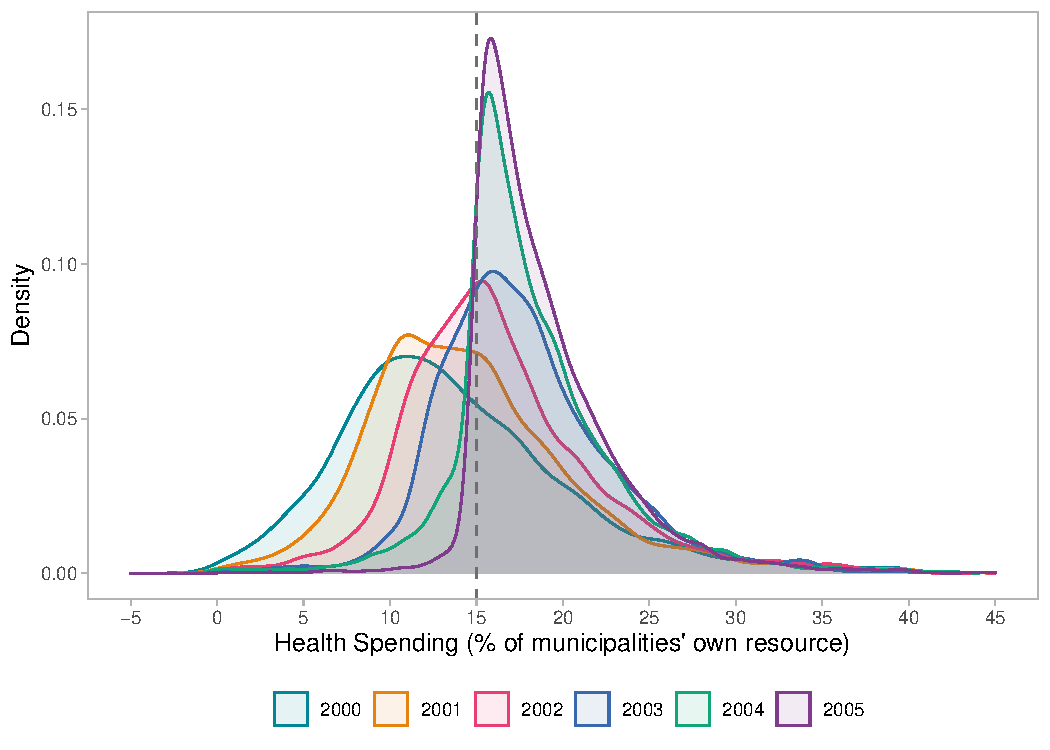
\includegraphics[width=\textwidth]{plots/hist_ec29.pdf}
    \end{subfigure}
        \begin{subfigure}{0.48\textwidth}
        \caption{\scriptsize Health Spending per capita (2010 R\$)}\label{fig:density_b}
        \centering
        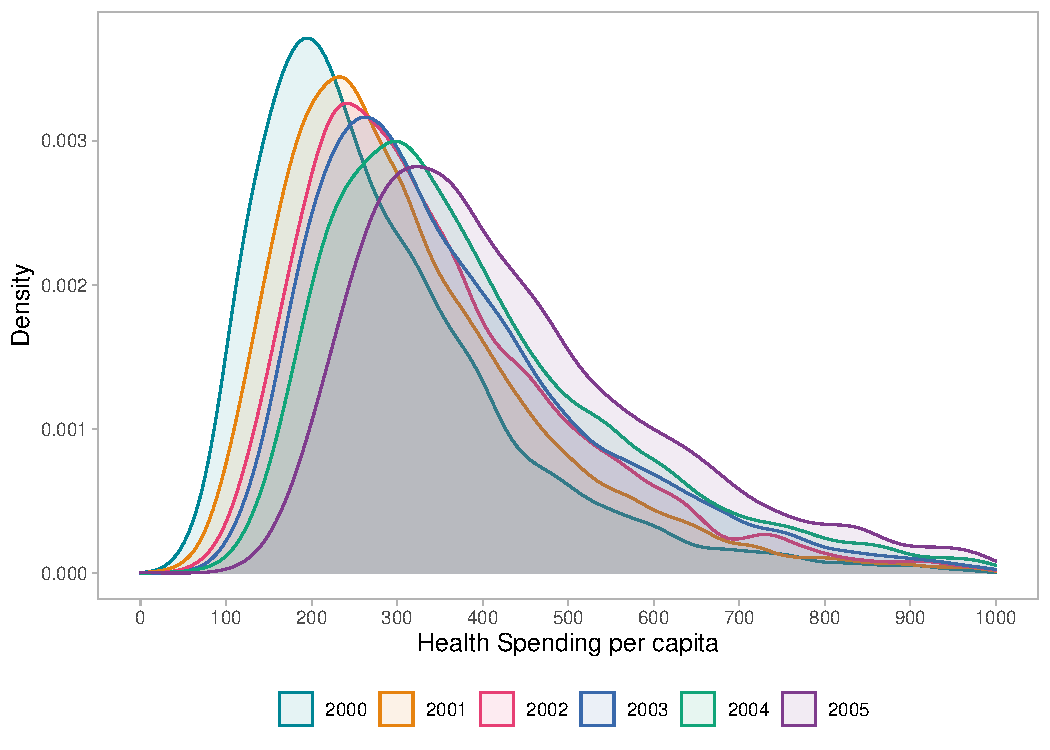
\includegraphics[width=\textwidth]{plots/hist_pc.pdf}
    \end{subfigure}
    \end{center}\vspace{+1pt}
\end{figure}


\subsection{Municipalities Health Expenditure after the EC/29}

Figure \ref{fig:density_a} shows the distribution of municipalities according to their share of own resources spent in public health. While in 2000, our baseline year, most of the municipalities spent less than 15\%, in 2005 the great majority of municipalities were complying with the target stipulated by the EC/29. Figure \ref{fig:density_b} presents the distribution of municipalities according to their health spending per capita (in 2010 R\$). One could suggest two facts about this figure. First, there was a significant increase in the average health spending per capita and second, there was also some increase in the inequality of health spending per capita across municipalities.\footnote{\cite{Piola2013} highlights that the EC/29 provided a broad definition of health care that led some states and municipalities to include in this account expenditures that should not be considered part of expenditures related to the provision of public health services by the SUS.}


Figure \ref{fig:2} present trends in health spending at the municipality level converted into indices set at 100 in 2000, for the bottom and top quartile of the distribution of the share of own resources spent in health care. Figure \ref{fig:2a} shows that the municipalities in the bottom of the distribution presented much higher increase in health spending relative to the municipalities on the top of the distribution. Moreover, as shown in Figure \ref{fig:2b} and \ref{fig:2c}, expenditure coming from own resources explains almost all the difference in the health spending increase between the bottom and top quartile. Figure \ref{fig:3} plots trends for health spending per capita by source. Own resources has always been the main source of public health spending for municipalities, but the trends suggest that it gain even more importance after the EC/29 (Figure \ref{fig:3a}). In the baseline year of 2000, health spending per capita in the bottom quartile was half of the top quartile. Figures \ref{fig:3b} and \ref{fig:3b} suggest that all these difference comes from differential own resource spending. \cite{Piola2013} shows that states and municipalities own resource spending was responsible for about two thirds of the increase in health spending between 2000 and 2011.


\begin{figure}[h]
    \begin{center}
    \caption{\footnotesize Health Spending Trends}\label{fig:2}
    \begin{subfigure}{.9\textwidth}
        \caption{\scriptsize Total Health Spending (2000 = 100)}\label{fig:2a}
        \centering
        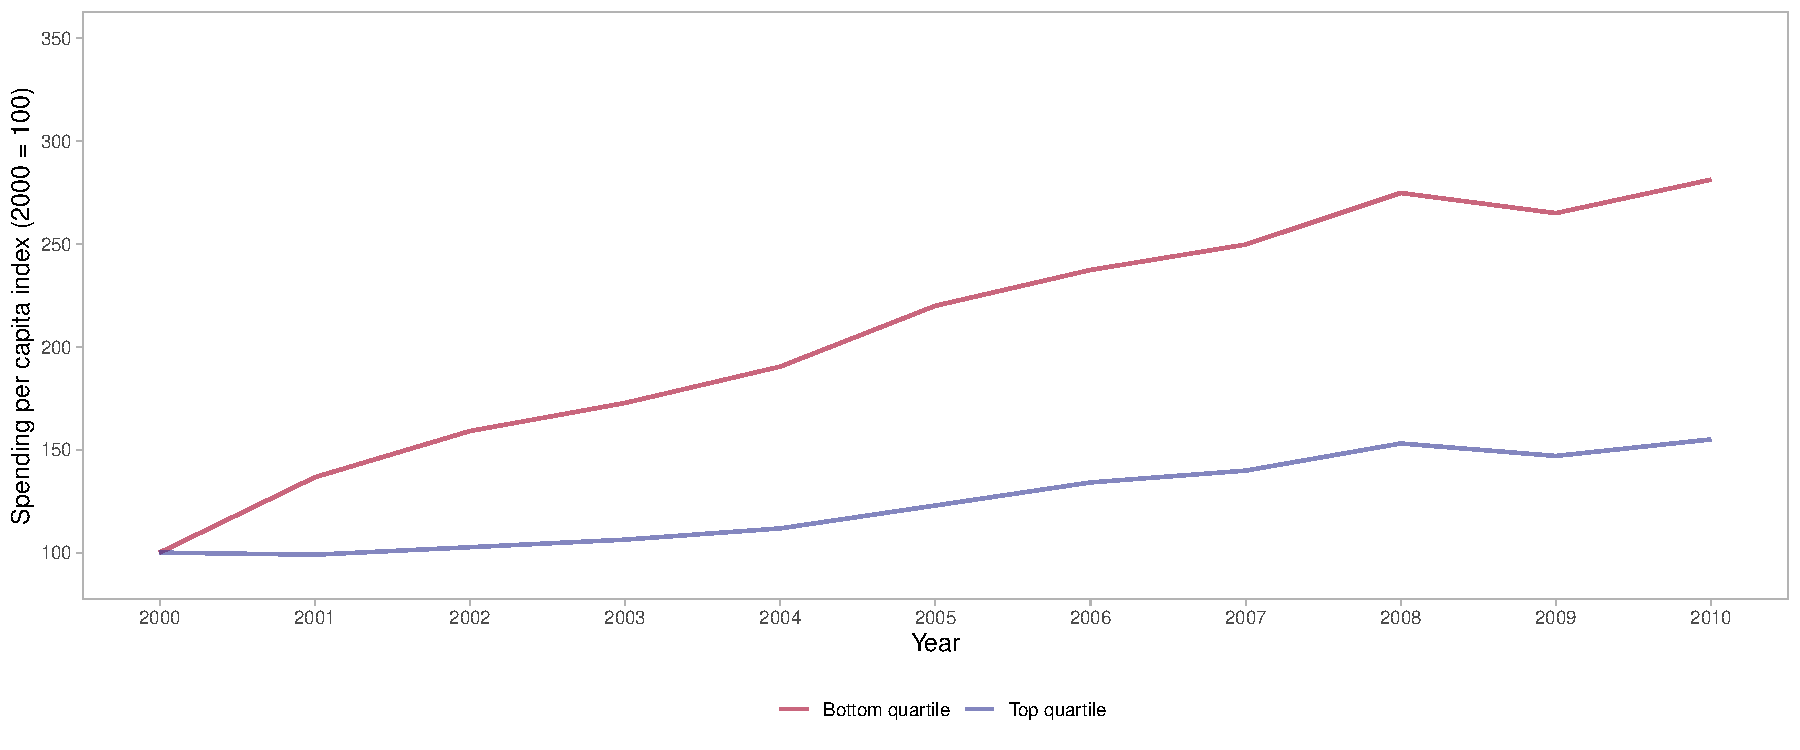
\includegraphics[width=\textwidth]{plots/plot_total.pdf}
    \end{subfigure}
        \begin{subfigure}{0.45\textwidth}
        \caption{\scriptsize Health Spending from Own Resources (2000 = 100)}\label{fig:2b}
        \centering
        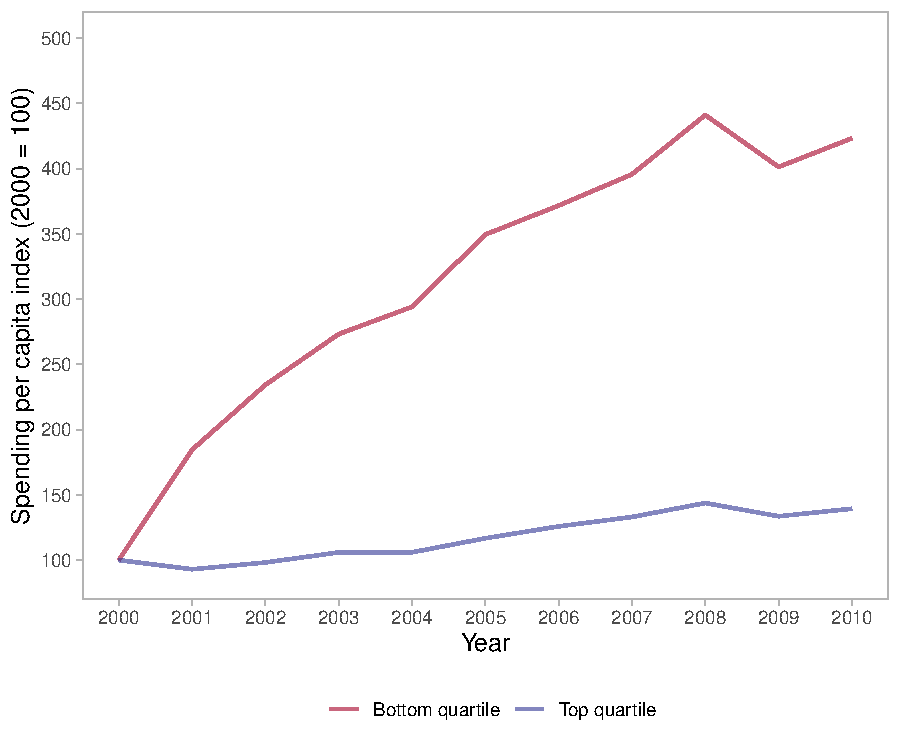
\includegraphics[width=\textwidth]{plots/plot_own.pdf}
    \end{subfigure}
        \begin{subfigure}{0.45\textwidth}
        \caption{\scriptsize Health Spending from Transfers (2000 = 100)}\label{fig:2c}
        \centering
        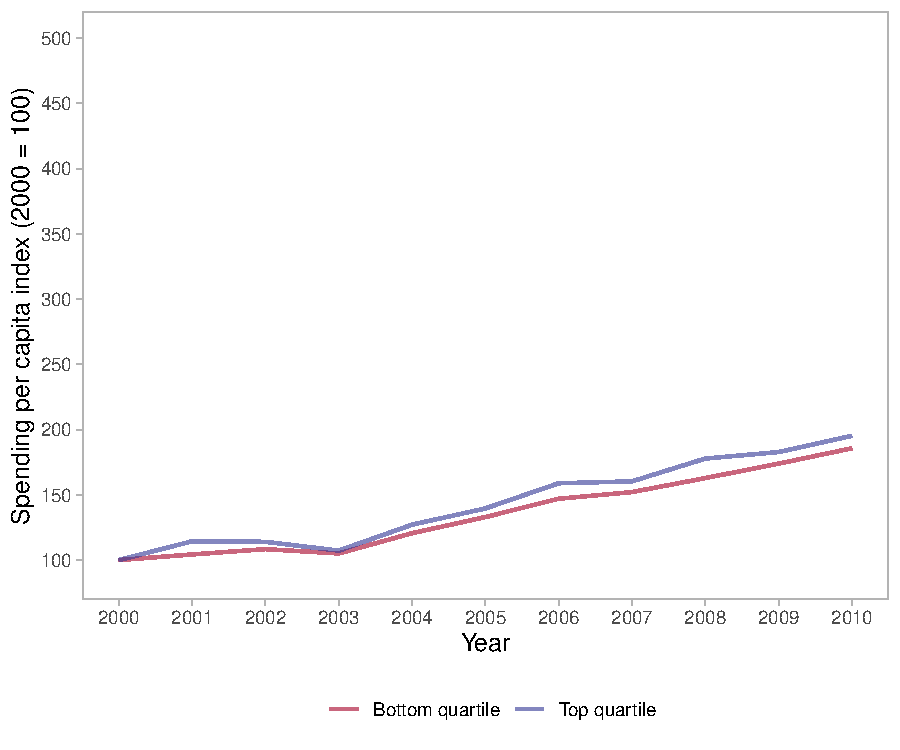
\includegraphics[width=\textwidth]{plots/plot_transf.pdf}
    \end{subfigure}
    \end{center}\vspace{+1pt}
\end{figure}

\begin{figure}[h]
    \begin{center}
    \caption{\footnotesize Health Spending Trends}\label{fig:3}
    \begin{subfigure}{.9\textwidth}
        \caption{\scriptsize Health Spending by Source (R\$2010) - Full Sample}\label{fig:3a}
        \centering
        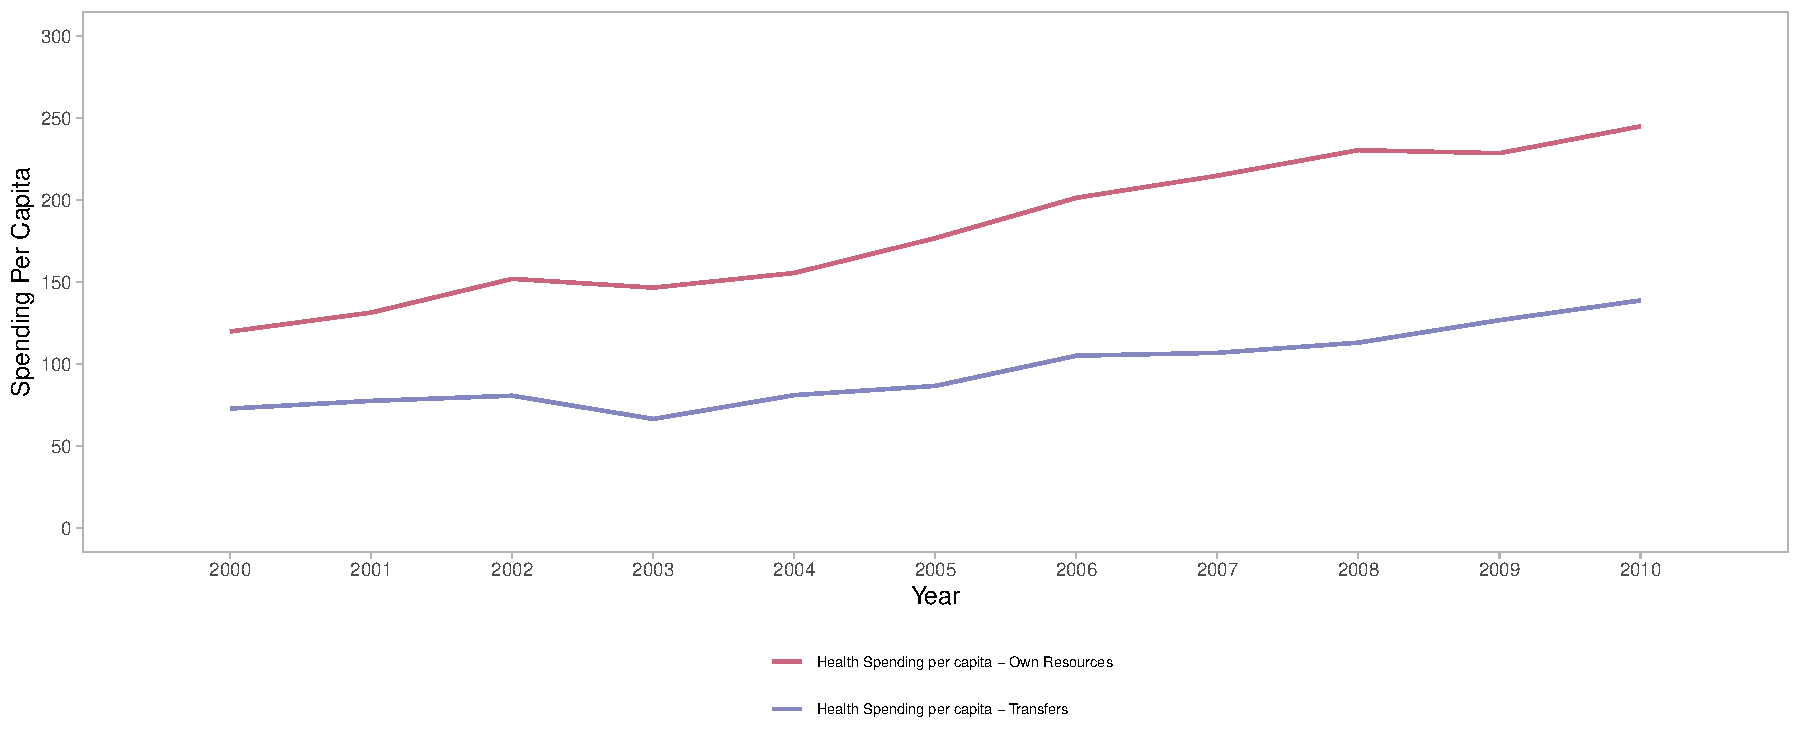
\includegraphics[width=\textwidth]{plots/plot_siops_level_source.pdf}
    \end{subfigure}
        \begin{subfigure}{0.45\textwidth}
        \caption{\scriptsize Health Spending by Source (R\$2010) - Bottom Quartile}\label{fig:3b}
        \centering
        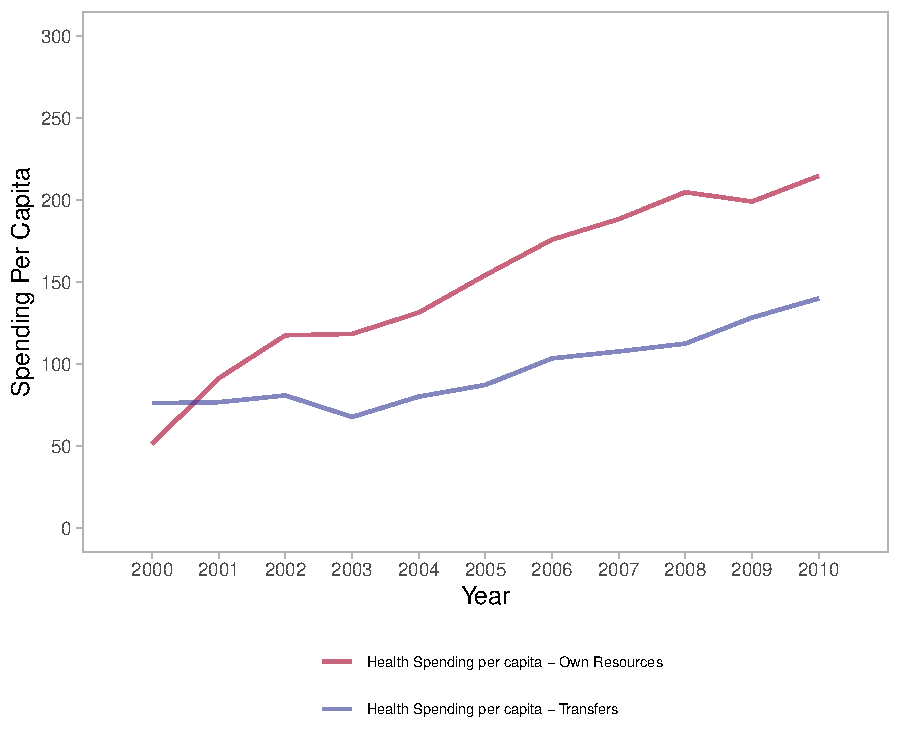
\includegraphics[width=\textwidth]{plots/plot_siops_level_source_bottom.pdf}
    \end{subfigure}
        \begin{subfigure}{0.45\textwidth}
        \caption{\scriptsize Health Spending by Source (R\$2010) - Top Quartile)}\label{fig:3c}
        \centering
        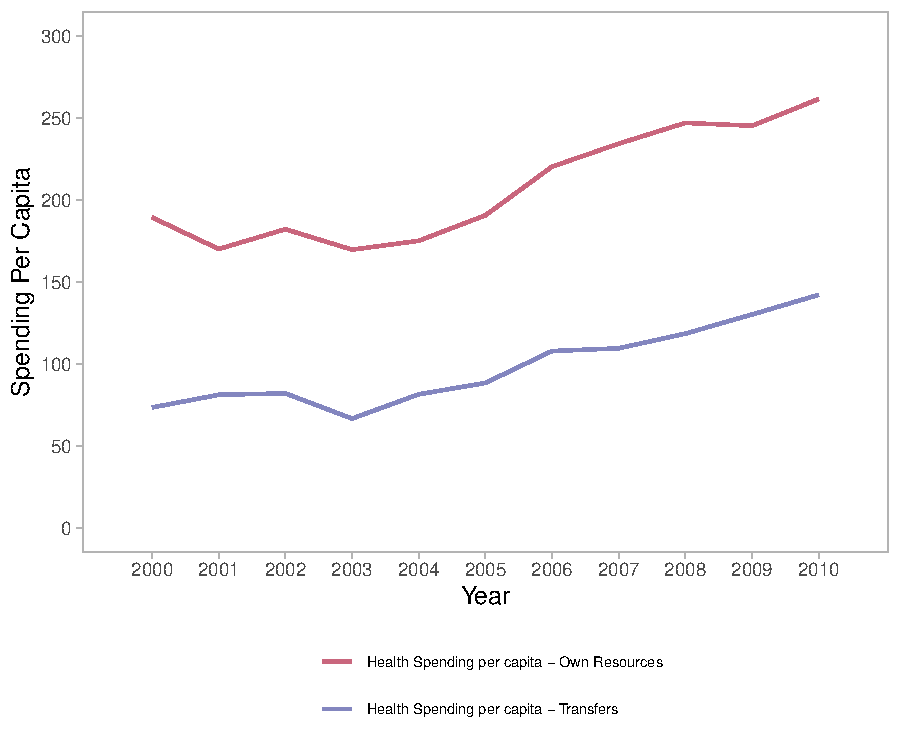
\includegraphics[width=\textwidth]{plots/plot_siops_level_source_top.pdf}
    \end{subfigure}
    \end{center}\vspace{+1pt}
\end{figure}


Moreover, municipalities' baseline level of own resource spending in health presents ample variation and is somewhat predictive of the change in total health spending per capita, which will be crucial to our identification strategy. Figure \ref{fig:4} plots, for all municipalities, the distance in percentage points to the EC/29 own resource spending target\footnote{We choose to work with the distance the target instead of the share of own resource expenditure in health in order to have easier to interpret estimates, as this measures presents a positive correlation with health spending} versus the change in total health spending per capita between 2000 and 2005. Consistently with the evidence presented in figure \ref{fig:2} and \ref{fig:3}, increases in health spending were larger in places with initially low levels of own resource spending, with a moderate to strong correlation of $0.45$.



\begin{figure}[h]
\begin{center}
    \caption{Changes in Health Spending per capita (2000-2005)}
    \scalebox{0.7}{
    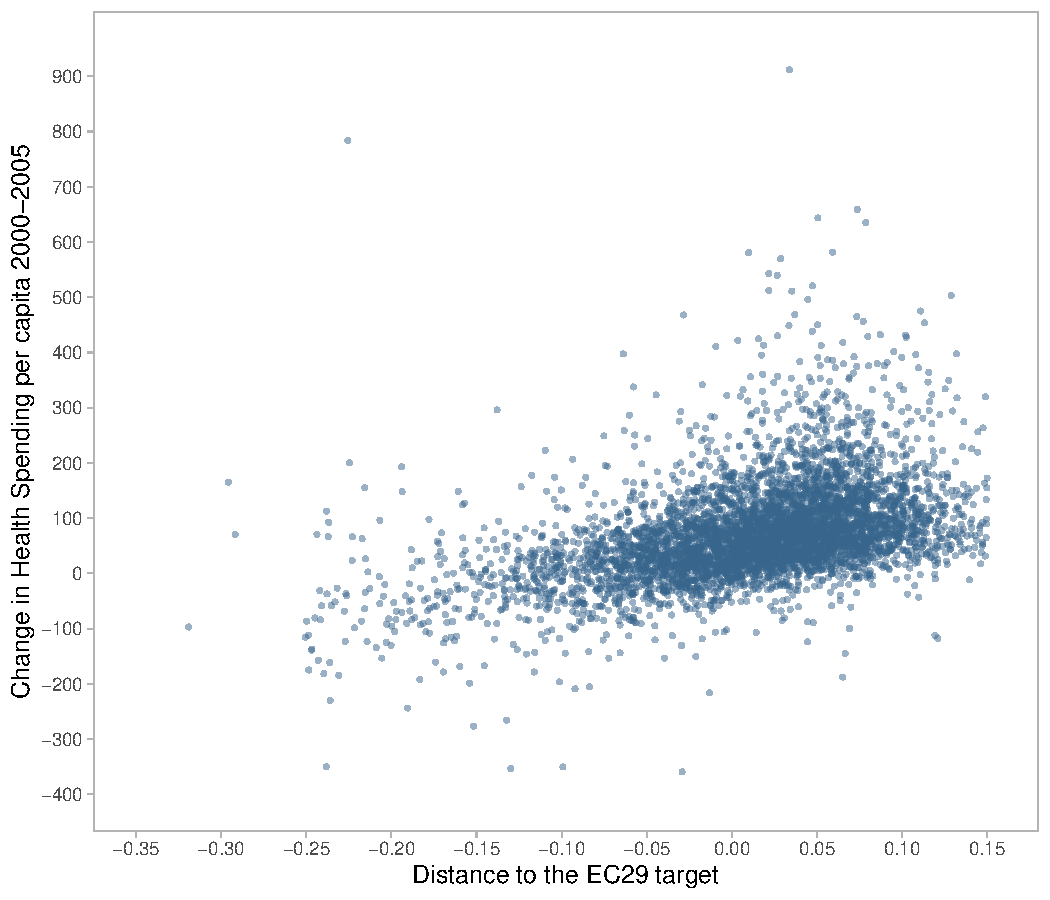
\includegraphics{plots/scatter_dist_ec29_baseline_change05.pdf}
    \label{fig:4}
    }
\end{center}
\end{figure}

In general, the descriptive evidence suggests that the EC/29 was responsible for bringing more resources to the provision of public health services and increasing the direct participation of states and municipalities in the financing of health care.

\section{Data}\label{sec:data}
\setstretch{1.5}

Table \ref{table:stats} presents summary statistics at the baseline year for all the variables used in this analysis: variables related to the EC2/9, fiscal data, health inputs, infant mortality rates, birth outcomes, and control variables. Statistics are presented for the full sample, and for the bottom and top quartile of distribution of municipalities' own resource spending in public health.

\subsection{EC/29 and Fiscal Data}

For evaluating the causal impact of the EC/29 on public spending, we combine public spending data from the Brazilian Finance System (FINBRA)\footnote{All spending data is presented in 2010 R\$. We used the General Price Index (IGP) to correct values}, which covers the period of 1998 to 2010, with data from the Brazilian National System of Public Health Budget (Datasus/SIOPS)\footnote{SIOPS was created right after the EC/29 to monitor revenues and expenditure in the provision of health care at the state and municipal levels, and to monitor compliance with the EC/29.} available from 2000 onward. FINBRA provides data on total public spending, spending by type, and spending by a few aggregated categories, such as Health and Sanitation, Education and Culture, etc, and SIOPS provides data on total health spending, health spending from own resources, health spending from intergovernmental transfers, spending by type, and the share of own resources spent in health.  Additionally, we also gather data on total public revenues and revenues by source (tax or intergovernmental transfers) from FINBRA.


Figure \ref{fig:5} displays the spatial variation in the share of own resources spent in health. Municipalities below the EC/29 are represented with colors in the red scale, while municipalities above the target are represented with the blue scale. The map shows significant differences in the share of own resources spent in health within the same state, providing the identifying variation of this study as we include state fixed-effects in our main specification. 

\begin{figure}[h!]
\begin{center}
    \caption{EC/29 Compliance Geographic Variation}
    \scalebox{0.7}{
    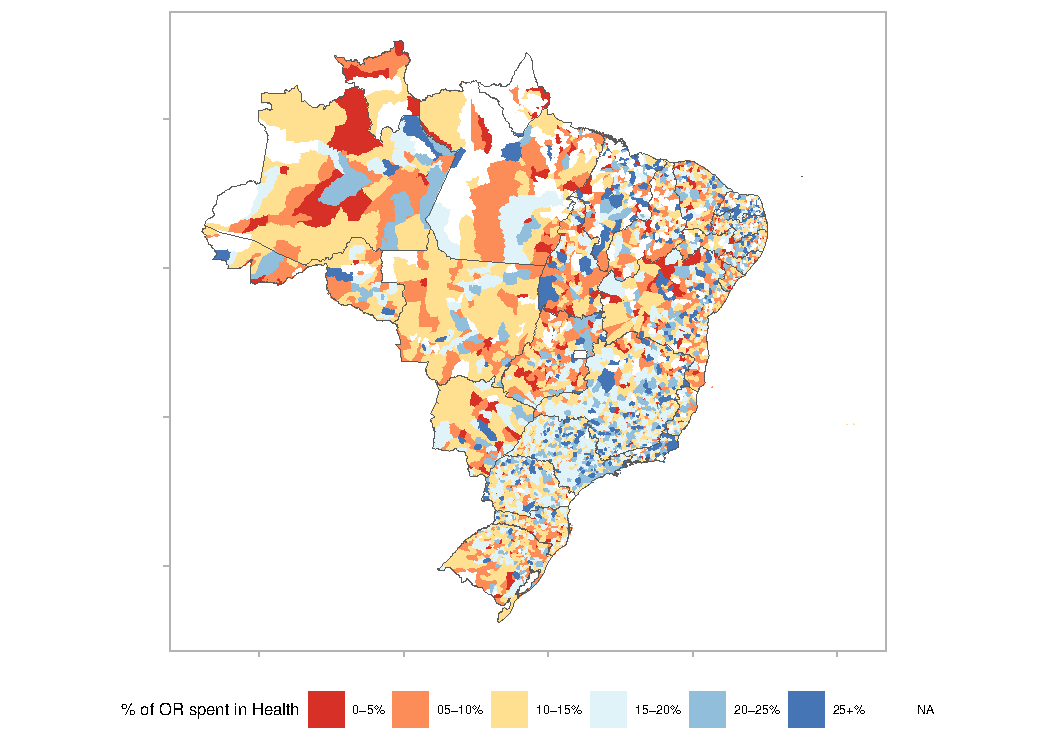
\includegraphics{plots/ec29_map.pdf}
    \label{fig:5}
    }
\end{center}
\end{figure}

\subsection{Infant Mortality and Birth Outcomes}

We use micro-data from Brazilian National System of Mortality Records (Datasus/SIM) and from the Brazilian National System of Birth Records (Datasus/SINASC) to construct Infant Mortality Rates. These micro-data allow us to construct Infant Mortality Rates by timing of death, and for the main causes of death. Moreover, following \cite{alfradique2009internaccoes} classification we are able to construct mortality rates amenable and non-amenable to primary care.

The SINASC micro-data records all births in Brazil and provides detailed information on these births, such as Apgar 1 and 5, birth weight and gestation weeks.

\subsection{Health Inputs}

There is no data available on municipalities' supply of public health infrastructure for the period of this analysis. However, we are able to indirectly construct proxies for public health infrastructure using the micro-data from the National System of Information on Ambulatory Care (Datasus/SIA). This database records every ambulatorial procedure funded by SUS, with information on the type and complexity of the procedure, the health professional responsible, and the corresponding health facility register number. Using this data we are able to calculate the number of health facilities with ambulatory service in a municipality, as well as the number of facilities with ambulatory services classified by the type of service and professional responsible for the service \footnote{We are able to construct these variables only for the period of 1998 to 2007, as changes in the SIA classification of ambulatorial procedures changes in 2008.}. Variables on the access to healthcare were constructed using data from the Brazilian National System of Information on Primary Care (Datasus/SIAB) and from SINASC. Primary care coverage at the intensive and extensive margin data comes from SIAB and data on the access to health services from SINASC. Lastly, we use SIA micro-data to build data on ambulatory production.

\subsection{Controls}

Our control variables can be classified into two different categories: socioeconomic controls and fiscal controls. The first, comes from the Census of 2000. The later, from FINBRA dataset. We use as fiscal controls the average health spending per capita in the bordering municipalities\footnote{cite Mattos article} and a dummy that indicates whether a municipalities spend more than 60\% of its revenue with personnel, non complying with the Fiscal Responsibility Law of 2000.


\section{Empirical Approach}\label{sec:emp}
\setstretch{1.5}

We estimate the effects of the EC/29 using a difference-in-difference (DiD) design with a continuous treatment, exploiting within-municipality variation. Intuitively, we compare the evolution of outcomes in municipalities far from the EC/29 15\% target with municipalities that were already complying with the target. The underlying assumption is that changes in outcomes for the later group provide a good counterfactual for changes that would have been observed in the former group had they been complying with the target. 

The identification relies on the cross-municipality variation in the share of own resource spent in the provision of healthcare and on the exogeneity of the EC/29 approval. Our approach to estimate the effect of the EC/29 correspond to the following equation:

\begin{equation} \label{eq:1}
    Y_{mts} = \beta \, Dist_{m,pre} \times Post_t  +  \delta_{st} + \delta_j + \epsilon_{mts} + \theta \, Z_{m,pre} + \gamma \, X_{mts}
\end{equation}

were $Y_{mts}$ is an outcome of interest in municipality $m$, state $s$, year $t$; $Dist_{m,pre}$ is the baseline percentage points distance to EC/29 target in municipality $m$; $Post_t$ is a dummy that equals one if the year is 2001 or above. $\delta_{st}$ and $\delta_j$ represent state-year fixed effects and municipality fixed effects. Additionally we include and an interaction between socioeconomic baseline controls and time, $\theta Z_{j,pre} * \delta_{t}$, and time varying fiscal controls, $X_{mts}$. Standard errors are cluster at the municipality level and the parameters of interest are the $\beta$'s.

We choose to work with the distance to the EC/29 target instead of the share of own resource spent in health for the ease of interpretation, as the distance positively correlates with changes in health spending. The inclusion of state-year fixed effects accounts for state-specific policies that might coincidentally affect outcomes in all municipalities within a state, and for the fact that some health policies and institutions are decentralized to state governments in Brazil. The time varying fiscal controls include compliance with the Fiscal Responsibility Law (LRF) \citep{lrf} and average health spending per capita in the neighboring municipalities. The LRF determines that municipalities must spend less than 60\% of its revenue in personnel. Municipalities not complying or close to the 60\% cap might have different incentives when increasing spending relative the municipalities complying with the LRF. \cite{castro2021effects} shows that health spending presents strong spatial externalities in Brazil, with neighbouring municipalities benefiting from better health outcomes, which highlights the importance of including this control.

\subsection{Validity of the Research Design}

Recent advances in econometric theory point out to several drawbacks in the two way fixed effects regressions generally used by empirical researches. \cite{callaway2021difference} highlights that DiD models with continuous treatment may require stronger parallel trends assumptions, as comparisons between different intensities of treatment can also be confounded by selection bias. Unlike usual DiD, this bias comes from the heterogeneity in treatment effects. If group of units have difference response to a certain dosage of treatment, the DiD will be contaminated by the differences in expected returns for these different dosage groups. Moreover, this bias persists even under traditional parallel trends assumption. For the estimator to be unbiased, we also need treatment effects across different dosage groups to be homogeneous at the same dosage. 

Like the classic DiD, under randomization of treatment dosage, this stronger parallel trends assumption is satisfied, as groups do not choose dosage levels based on expected returns. But, differently from the classic DiD, there is still no clear way to verify whether this assumption is satisfied. In this study, treatment was not randomized, but we argue that is quite exogenous and it is very unlikely that municipalities chose their distance to the spending target established by the EC/29 based on expected increases in health spending per capita. 

First, the process of approval of the EC/29 involved several political stages and actors and it was arguably quite difficult to predict when the proposals would become an amendment, what exactly would define, and how it would affect municipalities' public health spending decisions. Lastly, the strong relationship between baseline distance to the target and changes in health spending per capita presented in Figure \ref{fig:4} suggests that the constitutional amendment was binding\footnote{According to the Ministry of Health Financial Management Manual (Minitério da Saúde \citeyear{msmanual}), non-compliance with the minimum amount of resources that should be spent in the provision of healthcare can lead to sanctions similar to those imposed by the Fiscal Responsibility Law, such as retention of resources from the Municipalities’ Participation Fund and States’ Participation Fund, suspension of a term of office, and even Federal intervention.}. Therefore, it is fair to say that changes in spending across different distance to the target groups would probably be the same for a specific distance.

We are not able to empirically assess homogeneity in treatment effect, but we can still check for pre-trends and evaluate if classic parallel trends assumption holds in our case. For that, we estimate a variation of equation \ref{eq:1}, that allows for more flexible coefficient estimates:

\begin{equation} \label{eq:2}
\begin{aligned}
    Y_{mts} \, =  \, & \sum\limits_{i=1}^I \beta_{pre,i} \, Dist_{m,pre} \times EC29_{t+i} \, + \, \sum\limits_{j=0}^J \beta_{j} \, Dist_{m,pre} \times EC29_{t-j} \\  
             & +  \delta_{st} + \delta_m + \epsilon_{mts} + \, \theta \, Z_{m,pre} \times \delta_{t} + \gamma \, X_{mts}
\end{aligned}
\end{equation}

where $EC29_{t-j}$ are year specific indicators for whether EC/29 was enacted in year $t-j$; in like manner $EC29_{t+i}$ are specific year indicators for whether EC/29 was enacted in year $t+i$, that captures pre-trends in the outcome variable. The equation \ref{eq:2} also allow us to evaluate the dynamics through the years following the EC/29. 

Build in point on multiple hypothesis correction.  This will be important here....  \citet{RomanoWolf2005,Anderson2008}.








\section{Empirical Findings}\label{sec:emp}
\setstretch{1.5}

\subsection{Municipalities' Fiscal Response}

\begin{table}[H]
\begin{footnotesize}
\begin{center}
\scalebox{1}{
\begin{threeparttable}[b]

  \centering
  \caption{Causal Effects on Revenue}
    \begin{tabular}{rrcccrcccc}
          &       &       &       &       &       &       &       &       &  \\
    \midrule
          &       & \multicolumn{3}{c}{Revenue Per Capita} &       & \multicolumn{4}{c}{\% of Total Revenue} \\
\cmidrule{3-5}\cmidrule{7-10}          &       & \multicolumn{3}{c}{Distance to EC9 target} &       & \multicolumn{4}{c}{Distance to EC9 target} \\
\cmidrule{3-5}\cmidrule{7-10}          &       & (1)   & (2)   & (3)   &       & (1)   & (2)   &       & (3) \\
    \midrule
    \multicolumn{1}{p{15.145em}}{\textbf{Public Revenue}} &       &       &       &       &       &       &       &       &  \\
    \multicolumn{1}{l}{\multirow{2}[0]{*}{Total Revenue}} &       & -30.055 & -300.36 & -240.794 &       &       &       &       &  \\
          &       & (250.503) & (292.199) & (286.476) &       &       &       &       &  \\
    \multicolumn{1}{p{15.145em}}{\textbf{By Source}} &       &       &       &       &       &       &       &       &  \\
    \multicolumn{1}{l}{\multirow{2}[0]{*}{Tax Revenue}} &       & -10.107 & -8.649 & -91.432* &       & -0.007 & -0.022 &       & -0.018 \\
          &       & (55.028) & (51.705) & (54.064) &       & (0.04) & (0.031) &       & (0.028) \\
    \multicolumn{1}{l}{\multirow{2}[0]{*}{Transfers Revenue}} &       & -23.331 & -313.399 & -141.228 &       & -0.017 & -0.003 &       & -0.01 \\
          &       & (209.669) & (250.939) & (247.521) &       & (0.048) & (0.042) &       & (0.04) \\
    \multicolumn{1}{l}{\multirow{2}[0]{*}{Other Revenues}} &       & 3.383 & 21.687 & -8.134 &       & 0.024 & 0.025 &       & 0.028 \\
          &       & (97.589) & (103.061) & (106.689) &       & (0.042) & (0.04) &       & (0.041) \\
          &       &       &       &       &       &       &       &       &  \\
    \multicolumn{1}{p{15.145em}}{N. Obs} &       & \multicolumn{3}{c}{64,219} &       & \multicolumn{4}{c}{64,219} \\
          &       &       &       &       &       &       &       &       &  \\
    \midrule
    \midrule
          &       &       &       &       &       &       &       &       &  \\
    \end{tabular}%
    
  \label{table:revenue}%

\end{threeparttable}
}
\end{center}
\end{footnotesize}
\end{table}

\begin{table}[H]
\begin{footnotesize}
\begin{center}
\scalebox{0.9}{
\begin{threeparttable}[b]

  \centering
  \caption{Causal Effects on Public Spending}
    \begin{tabular}{rrrrrrrrr}
          &       &       &       &       &       &       &       &  \\
    \midrule
          &       & \multicolumn{3}{c}{Spending Per Capita} &       & \multicolumn{3}{c}{\% of Total Spending} \\
\cmidrule{3-5}\cmidrule{7-9}          &       & \multicolumn{3}{c}{Distance to EC9 target} &       & \multicolumn{3}{c}{Distance to EC9 target} \\
\cmidrule{3-5}\cmidrule{7-9}          &       & \multicolumn{1}{c}{(1)} & \multicolumn{1}{c}{(2)} & \multicolumn{1}{c}{(3)} &       & \multicolumn{1}{c}{(1)} & \multicolumn{1}{c}{(2)} & \multicolumn{1}{c}{(3)} \\
    \midrule
    \multicolumn{1}{p{15.145em}}{\textbf{Public Spending}} &       &       &       &       &       &       &       &  \\
    \multicolumn{1}{l}{\multirow{2}[0]{*}{Total Spending}} &       & \multicolumn{1}{c}{168.709} & \multicolumn{1}{c}{-186.987} & \multicolumn{1}{c}{-161.444} &       &       &       &  \\
          &       & \multicolumn{1}{c}{(268.596)} & \multicolumn{1}{c}{(304.982)} & \multicolumn{1}{c}{(303.811)} &       &       &       &  \\
    \multicolumn{1}{p{15.145em}}{\textbf{By Type}} &       &       &       &       &       &       &       &  \\
    \multicolumn{1}{l}{\multirow{2}[0]{*}{Human Resources Spending}} &       & \multicolumn{1}{c}{306.195***} & \multicolumn{1}{c}{213.315} & \multicolumn{1}{c}{175.86} &       & \multicolumn{1}{c}{0.171***} & \multicolumn{1}{c}{0.16***} & \multicolumn{1}{c}{0.135***} \\
          &       & \multicolumn{1}{c}{(115.292)} & \multicolumn{1}{c}{(147.493)} & \multicolumn{1}{c}{(139.003)} &       & \multicolumn{1}{c}{(0.064)} & \multicolumn{1}{c}{(0.052)} & \multicolumn{1}{c}{(0.046)} \\
    \multicolumn{1}{l}{\multirow{2}[0]{*}{Investment Spending}} &       & \multicolumn{1}{c}{-137.637**} & \multicolumn{1}{c}{-77.742} & \multicolumn{1}{c}{-87.432} &       & \multicolumn{1}{c}{-0.092***} & \multicolumn{1}{c}{-0.004} & \multicolumn{1}{c}{-0.016} \\
          &       & \multicolumn{1}{c}{(59.934)} & \multicolumn{1}{c}{(58.115)} & \multicolumn{1}{c}{(62.058)} &       & \multicolumn{1}{c}{(0.035)} & \multicolumn{1}{c}{(0.026)} & \multicolumn{1}{c}{(0.027)} \\
    \multicolumn{1}{l}{\multirow{2}[0]{*}{Other Spending}} &       & \multicolumn{1}{c}{1.677} & \multicolumn{1}{c}{-318.72*} & \multicolumn{1}{c}{-241.234} &       & \multicolumn{1}{c}{-0.079} & \multicolumn{1}{c}{-0.156***} & \multicolumn{1}{c}{-0.118**} \\
          &       & \multicolumn{1}{c}{(203.992)} & \multicolumn{1}{c}{(192.711)} & \multicolumn{1}{c}{(176.37)} &       & \multicolumn{1}{c}{(0.069)} & \multicolumn{1}{c}{(0.054)} & \multicolumn{1}{c}{(0.046)} \\
    \multicolumn{1}{p{15.145em}}{\textbf{By Category}} &       &       &       &       &       &       &       &  \\
    \multicolumn{1}{l}{\multirow{2}[0]{*}{Health and Sanitation Spending}} &       & \multicolumn{1}{c}{240.446**} & \multicolumn{1}{c}{227.507**} & \multicolumn{1}{c}{229.54**} &       & \multicolumn{1}{c}{0.175***} & \multicolumn{1}{c}{0.166***} & \multicolumn{1}{c}{0.167***} \\
          &       & \multicolumn{1}{c}{(94.134)} & \multicolumn{1}{c}{(94.122)} & \multicolumn{1}{c}{(91.862)} &       & \multicolumn{1}{c}{(0.044)} & \multicolumn{1}{c}{(0.035)} & \multicolumn{1}{c}{(0.034)} \\
    \multicolumn{1}{l}{\multirow{2}[0]{*}{Transport Spending}} &       & \multicolumn{1}{c}{3.67} & \multicolumn{1}{c}{-85.314} & \multicolumn{1}{c}{-77.514} &       & \multicolumn{1}{c}{0.002} & \multicolumn{1}{c}{-0.042} & \multicolumn{1}{c}{-0.045*} \\
          &       & \multicolumn{1}{c}{(61.171)} & \multicolumn{1}{c}{(60.894)} & \multicolumn{1}{c}{(54.352)} &       & \multicolumn{1}{c}{(0.029)} & \multicolumn{1}{c}{(0.027)} & \multicolumn{1}{c}{(0.025)} \\
    \multicolumn{1}{l}{\multirow{2}[0]{*}{Education and Culture Spending}} &       & \multicolumn{1}{c}{126.236*} & \multicolumn{1}{c}{-7.015} & \multicolumn{1}{c}{-4.575} &       & \multicolumn{1}{c}{0.052} & \multicolumn{1}{c}{0.022} & \multicolumn{1}{c}{0.014} \\
          &       & \multicolumn{1}{c}{(74.761)} & \multicolumn{1}{c}{(112.71)} & \multicolumn{1}{c}{(105.408)} &       & \multicolumn{1}{c}{(0.038)} & \multicolumn{1}{c}{(0.04)} & \multicolumn{1}{c}{(0.034)} \\
    \multicolumn{1}{l}{\multirow{2}[0]{*}{Housing and Urban Spending}} &       & \multicolumn{1}{c}{1.846} & \multicolumn{1}{c}{7.284} & \multicolumn{1}{c}{14.39} &       & \multicolumn{1}{c}{-0.035} & \multicolumn{1}{c}{0.008} & \multicolumn{1}{c}{0.016} \\
          &       & \multicolumn{1}{c}{(74.606)} & \multicolumn{1}{c}{(68.773)} & \multicolumn{1}{c}{(66.042)} &       & \multicolumn{1}{c}{(0.046)} & \multicolumn{1}{c}{(0.038)} & \multicolumn{1}{c}{(0.036)} \\
    \multicolumn{1}{l}{\multirow{2}[0]{*}{Social Assistance Spending per capita}} &       & \multicolumn{1}{c}{-6.605} & \multicolumn{1}{c}{-23.11} & \multicolumn{1}{c}{-54.946} &       & \multicolumn{1}{c}{-0.036} & \multicolumn{1}{c}{-0.033**} & \multicolumn{1}{c}{-0.045***} \\
          &       & \multicolumn{1}{c}{(41.289)} & \multicolumn{1}{c}{(37.133)} & \multicolumn{1}{c}{(40.054)} &       & \multicolumn{1}{c}{(0.023)} & \multicolumn{1}{c}{(0.015)} & \multicolumn{1}{c}{(0.014)} \\
    \multicolumn{1}{l}{\multirow{2}[0]{*}{Spending in Other Categories per capita}} &       & \multicolumn{1}{c}{-193.062} & \multicolumn{1}{c}{-290.63**} & \multicolumn{1}{c}{-236.849*} &       & \multicolumn{1}{c}{-0.193***} & \multicolumn{1}{c}{-0.113**} & \multicolumn{1}{c}{-0.091**} \\
          &       & \multicolumn{1}{c}{(131.77)} & \multicolumn{1}{c}{(141.214)} & \multicolumn{1}{c}{(136.021)} &       & \multicolumn{1}{c}{(0.06)} & \multicolumn{1}{c}{(0.047)} & \multicolumn{1}{c}{(0.039)} \\
          &       &       &       &       &       &       &       &  \\
    \multicolumn{1}{p{15.145em}}{N. Obs} &       & \multicolumn{3}{c}{64,327} &       & \multicolumn{3}{c}{64,327} \\
          &       &       &       &       &       &       &       &  \\
    \midrule
    \midrule
          &       &       &       &       &       &       &       &  \\
    \end{tabular}%
    
  \label{table:spending_finbra}%

\end{threeparttable}
}
\end{center}
\end{footnotesize}
\end{table}

\begin{table}[H]
\begin{footnotesize}
\begin{center}
\scalebox{0.9}{
\begin{threeparttable}[b]

  \centering
  \caption{Causal Effects on Public Health Spending}
    \begin{tabular}{rrcccrcccc}
          &       &       &       &       &       &       &       &       &  \\
    \midrule
          &       & \multicolumn{3}{c}{Spending Per Capita} &       & \multicolumn{4}{c}{\% of Total Spending} \\
\cmidrule{3-5}\cmidrule{7-10}          &       & \multicolumn{3}{c}{Distance to EC9 target} &       & \multicolumn{4}{c}{Distance to EC9 target} \\
\cmidrule{3-5}\cmidrule{7-10}          &       & (1)   & (2)   & (3)   &       & (1)   & (2)   &       & (3) \\
    \midrule
    \multicolumn{1}{p{15.145em}}{\textbf{Public Health Spending}} &       &       &       &       &       &       &       &       &  \\
    \multicolumn{1}{l}{\multirow{2}[0]{*}{Total}} &       & 381.559*** & 399.331*** & 394.568*** &       &       &       &       &  \\
          &       & (59.903) & (75.697) & (64.079) &       &       &       &       &  \\
    \multicolumn{1}{p{15.145em}}{\textbf{By Source}} &       &       &       &       &       &       &       &       &  \\
    \multicolumn{1}{l}{\multirow{2}[0]{*}{Own Resources}} &       & 352.269*** & 405.494*** & 391.309*** &       & 1.056*** & 1.011*** &       & 0.996*** \\
          &       & (29.284) & (31.287) & (31.318) &       & (0.089) & (0.164) &       & (0.139) \\
    \multicolumn{1}{l}{\multirow{2}[0]{*}{Transfers}} &       & 27.149 & -8.477 & 1.442 &       & -1.056*** & -1.011*** &       & -0.996*** \\
          &       & (45.261) & (56.508) & (48.431) &       & (0.089) & (0.164) &       & (0.139) \\
    \multicolumn{1}{p{15.145em}}{\textbf{By Type}} &       &       &       &       &       &       &       &       &  \\
    \multicolumn{1}{l}{\multirow{2}[0]{*}{Human Resources}} &       & 156.998*** & 124.531*** & 116.553*** &       & 0.248*** & -0.035 &       & -0.076 \\
          &       & (30.937) & (35.672) & (30.81) &       & (0.085) & (0.103) &       & (0.084) \\
    \multicolumn{1}{l}{\multirow{2}[0]{*}{Investiment}} &       & 48.888*** & 63.988*** & 63.258*** &       & 0.125*** & 0.207*** &       & 0.194*** \\
          &       & (6.424) & (6.326) & (6.301) &       & (0.033) & (0.032) &       & (0.031) \\
    \multicolumn{1}{l}{\multirow{2}[0]{*}{3rd parties services}} &       & 43.452 & 28.185 & 28.918 &       & -0.338*** & -0.461** &       & -0.387** \\
          &       & (36.298) & (38.185) & (37.753) &       & (0.092) & (0.183) &       & (0.157) \\
    \multicolumn{1}{l}{\multirow{2}[0]{*}{Other Expenditures}} &       & 146.728*** & 197.11*** & 195.02*** &       & -0.034 & 0.317** &       & 0.281** \\
          &       & (28.285) & (39.834) & (33.272) &       & (0.09) & (0.128) &       & (0.119) \\
          &       &       &       &       &       &       &       &       &  \\
    \multicolumn{1}{p{15.145em}}{N. Obs} &       & \multicolumn{3}{c}{55,327} &       & \multicolumn{4}{c}{55,327} \\
          &       &       &       &       &       &       &       &       &  \\
    \midrule
    \midrule
          &       &       &       &       &       &       &       &       &  \\
    \end{tabular}%
    
  \label{table:spending_siops}%

\end{threeparttable}
}
\end{center}
\end{footnotesize}
\end{table}


\begin{figure}[h]
    \begin{center}
    \caption{Causal Effects on Revenues per capita}\label{fig:revenue1}
    \begin{subfigure}{0.49\textwidth}
        \caption{\scriptsize Total Revenue}\label{fig:rev1_a}
        \centering
        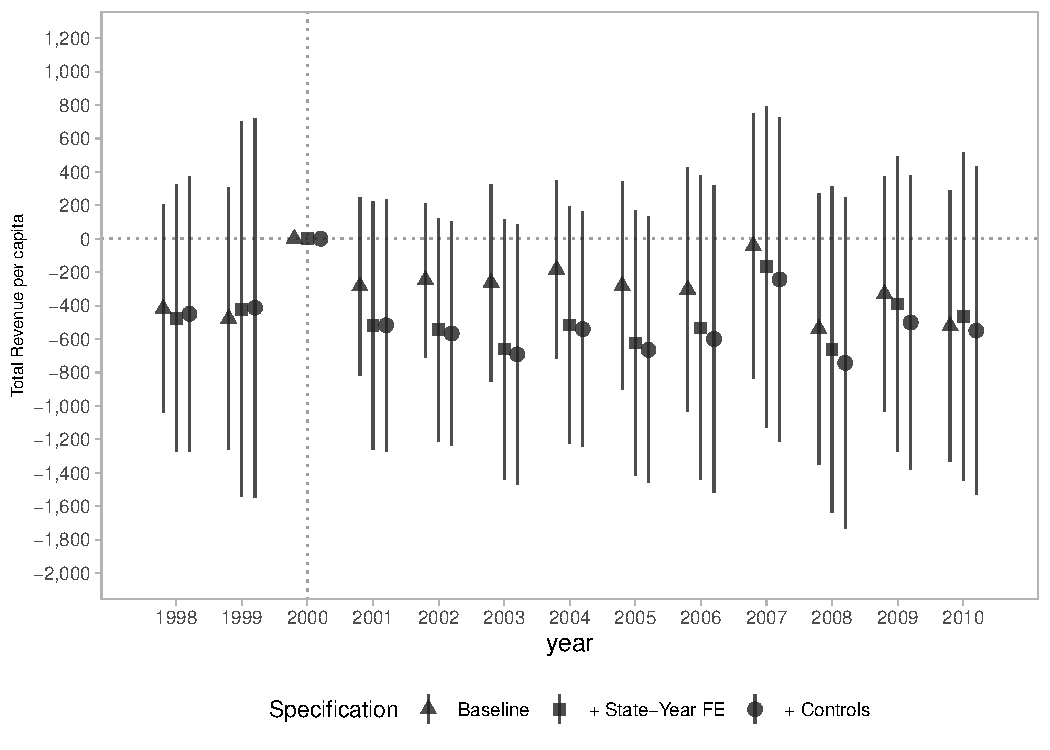
\includegraphics[width=\textwidth]{plots/spending/finbra_reccorr_pcapita_dist_ec29_baseline_dist_ec29_baseline_full.pdf}
    \end{subfigure}
    \begin{subfigure}{0.49\textwidth}
        \centering
        \caption{\scriptsize Tax Revenue}\label{fig:rev1_b}
        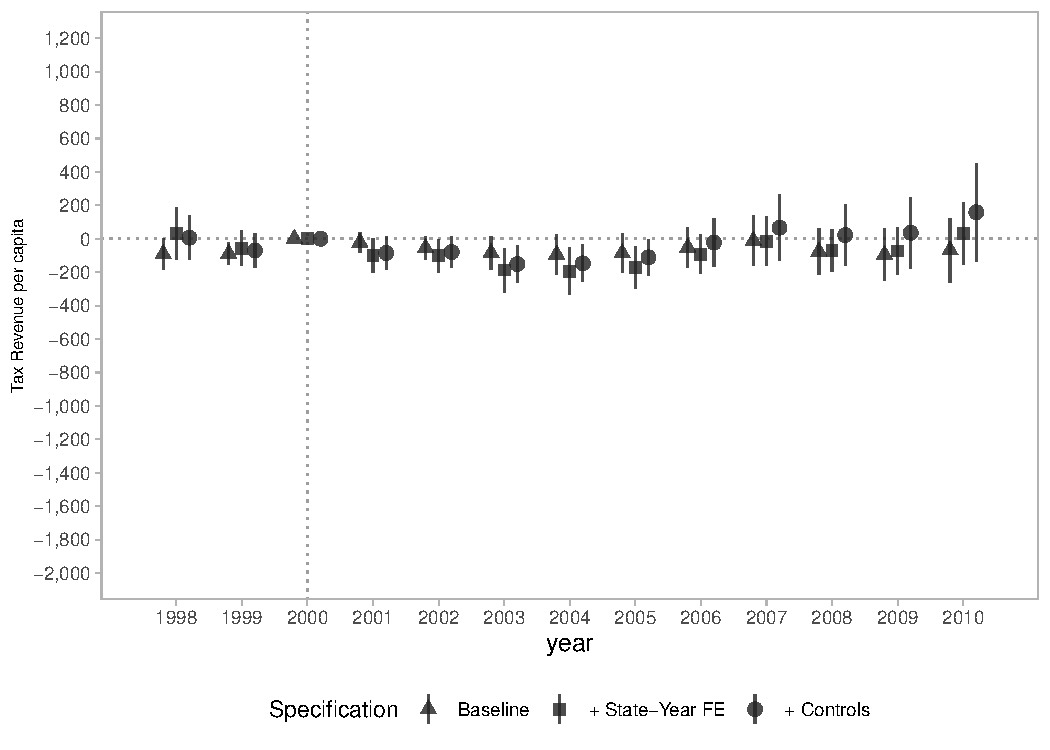
\includegraphics[width=\textwidth]{plots/spending/finbra_rectribut_pcapita_dist_ec29_baseline_dist_ec29_baseline_full.pdf}
    \end{subfigure}
    \begin{subfigure}{0.49\textwidth}
        \centering
        \caption{\scriptsize Transfers Revenue}\label{fig:rev1_c}
        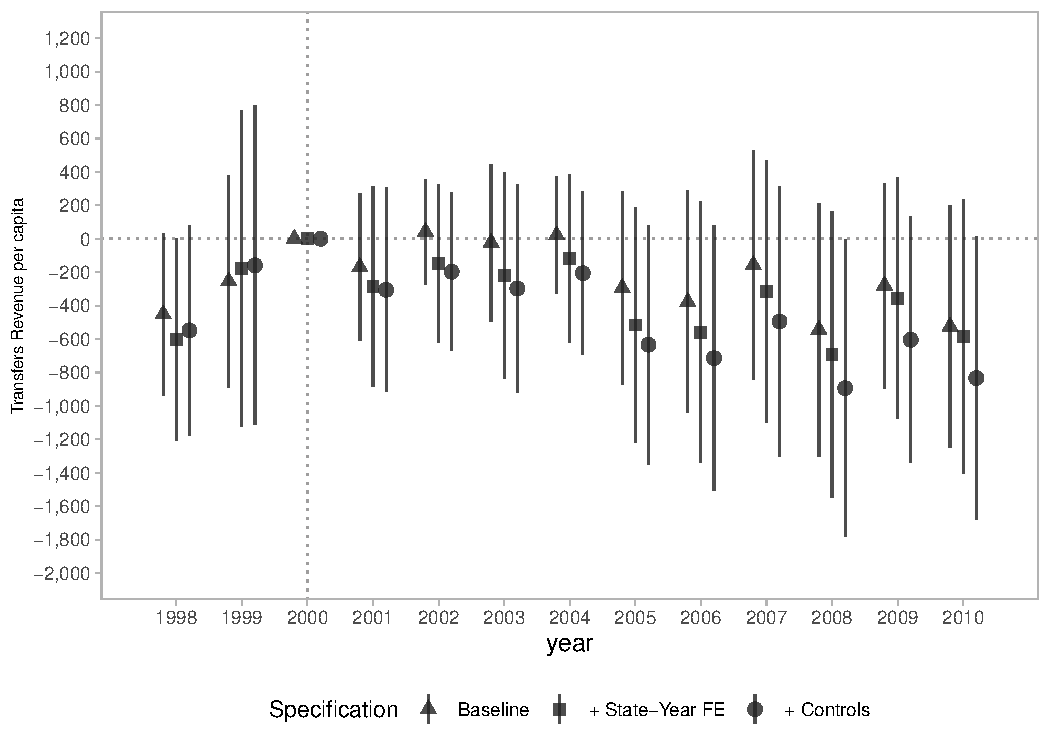
\includegraphics[width=\textwidth]{plots/spending/finbra_rectransf_pcapita_dist_ec29_baseline_dist_ec29_baseline_full.pdf}
    \end{subfigure}
    \begin{subfigure}{0.49\textwidth}
        \centering
        \caption{\scriptsize Other Revenue}\label{fig:rev1_d}
        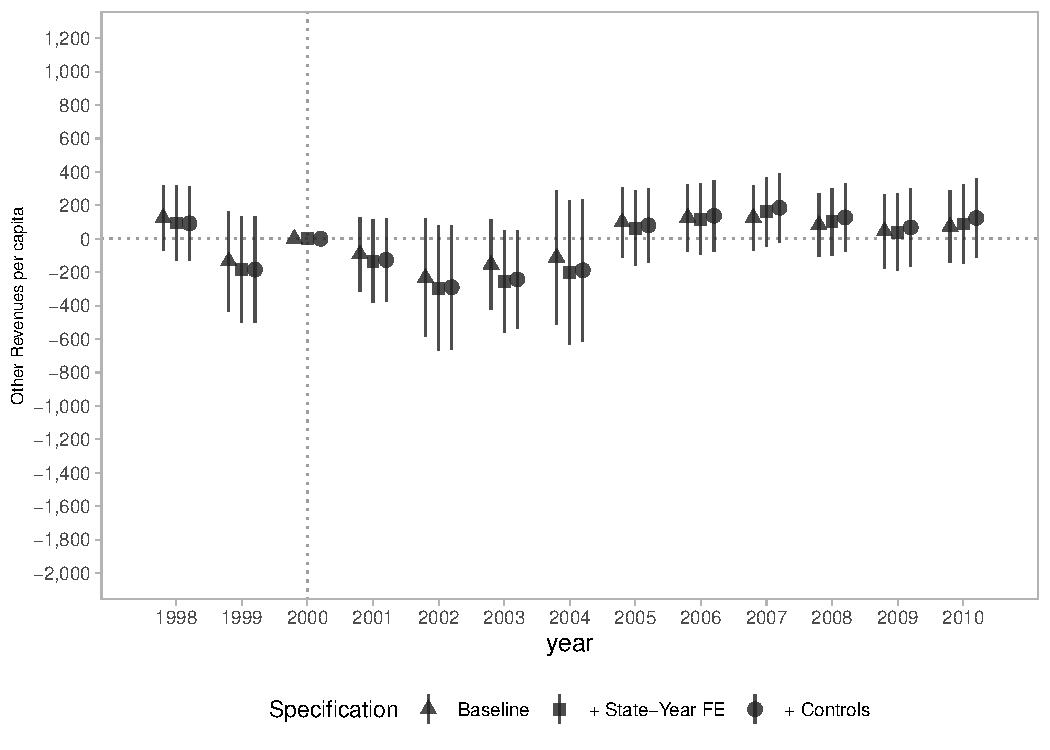
\includegraphics[width=\textwidth]{plots/spending/finbra_rec_outros_pcapita_dist_ec29_baseline_dist_ec29_baseline_full.pdf}
    \end{subfigure}
    
    \end{center}
    
\end{figure}

\begin{figure}[h]
    \begin{center}
    \caption{Causal Effects on Revenues (\% of Total Revenue)}\label{fig:revenue2}
    \begin{subfigure}{0.32\textwidth}
        \centering
        \caption{\scriptsize Tax Revenue}\label{fig:rev2_a}
        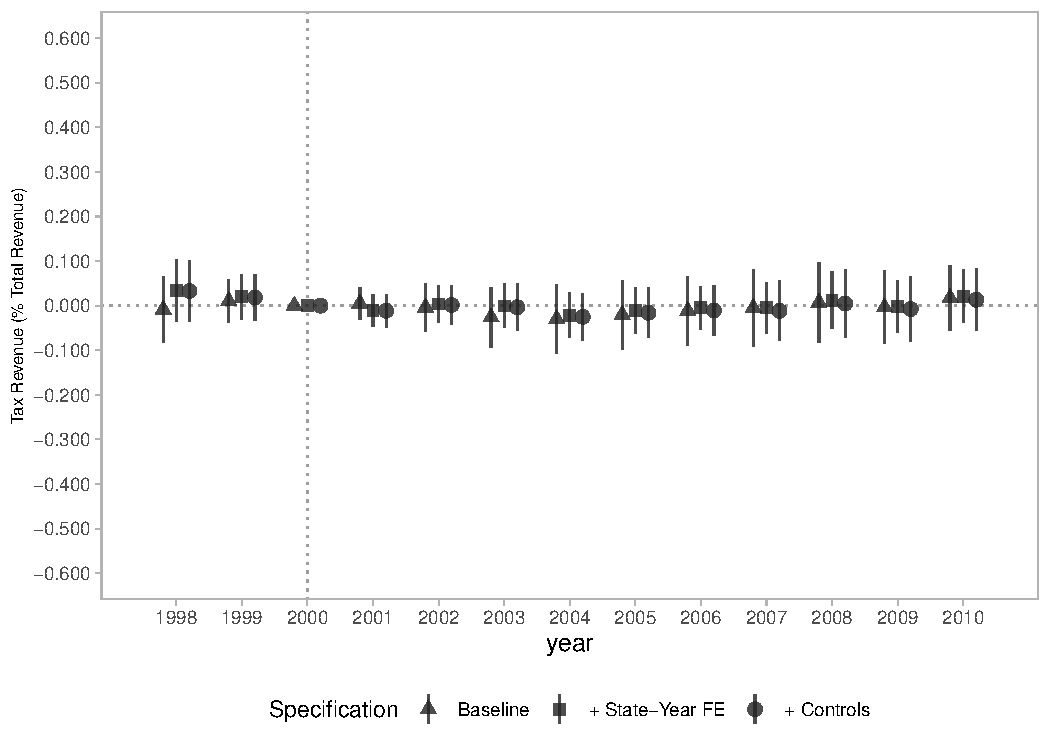
\includegraphics[width=\textwidth]{plots/spending/finbra_rectribut_share_dist_ec29_baseline_dist_ec29_baseline_full.pdf}
    \end{subfigure}
    \begin{subfigure}{0.32\textwidth}
        \centering
        \caption{\scriptsize Transfers Revenue}\label{fig:rev2_b}
        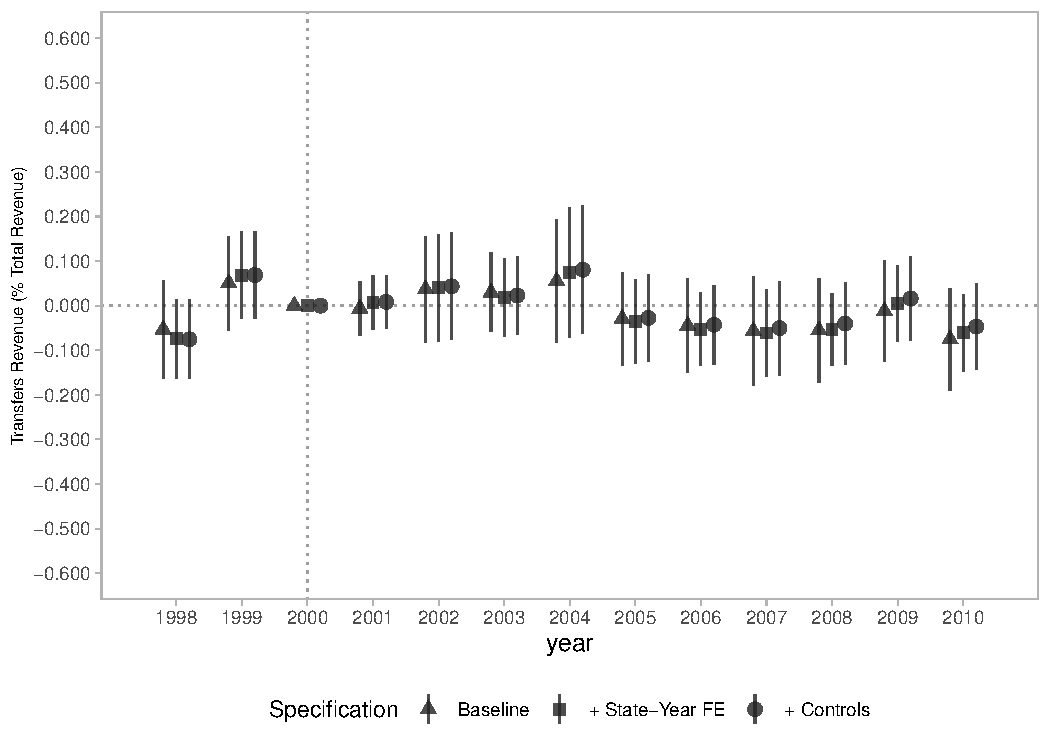
\includegraphics[width=\textwidth]{plots/spending/finbra_rectransf_share_dist_ec29_baseline_dist_ec29_baseline_full.pdf}
    \end{subfigure}
    \begin{subfigure}{0.32\textwidth}
        \centering
        \caption{\scriptsize Other Revenue}\label{fig:rev2_c}
        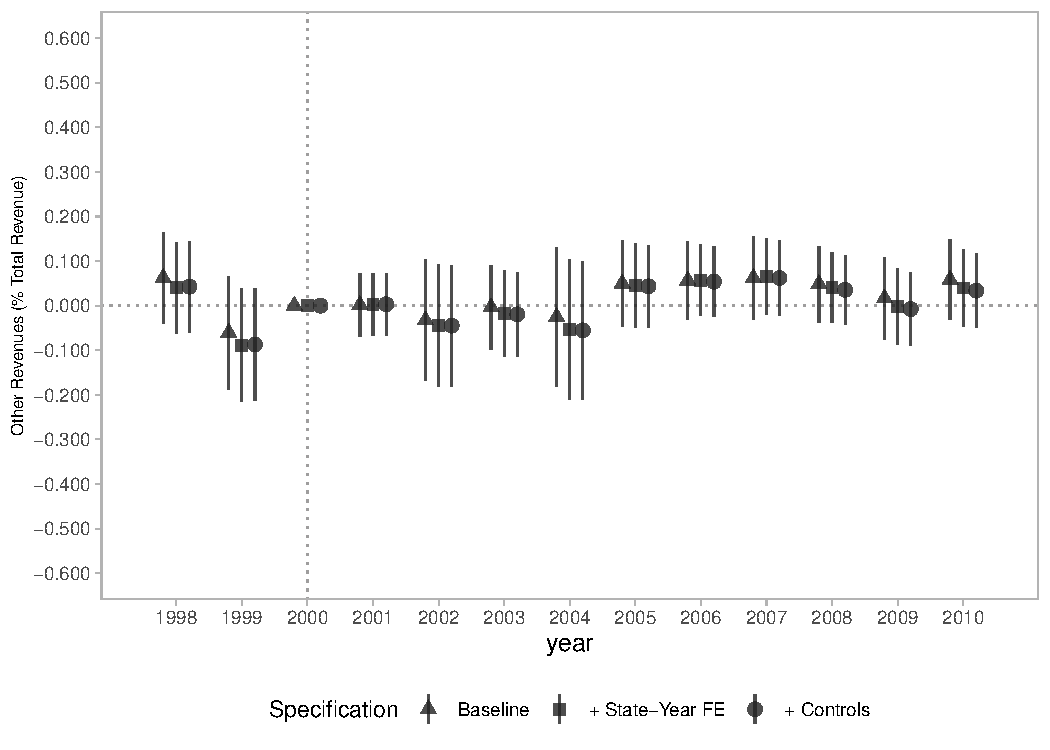
\includegraphics[width=\textwidth]{plots/spending/finbra_rec_outros_share_dist_ec29_baseline_dist_ec29_baseline_full.pdf}
    \end{subfigure}
    
    \end{center}
    
\end{figure}


\begin{figure}[h]
    \begin{center}
    \caption{Causal Effects on Public Spending per capita - By Type}\label{fig:finbra1}
    \begin{subfigure}{0.49\textwidth}
        \caption{\scriptsize Total Spending}\label{fig:finbra1_a}
        \centering
        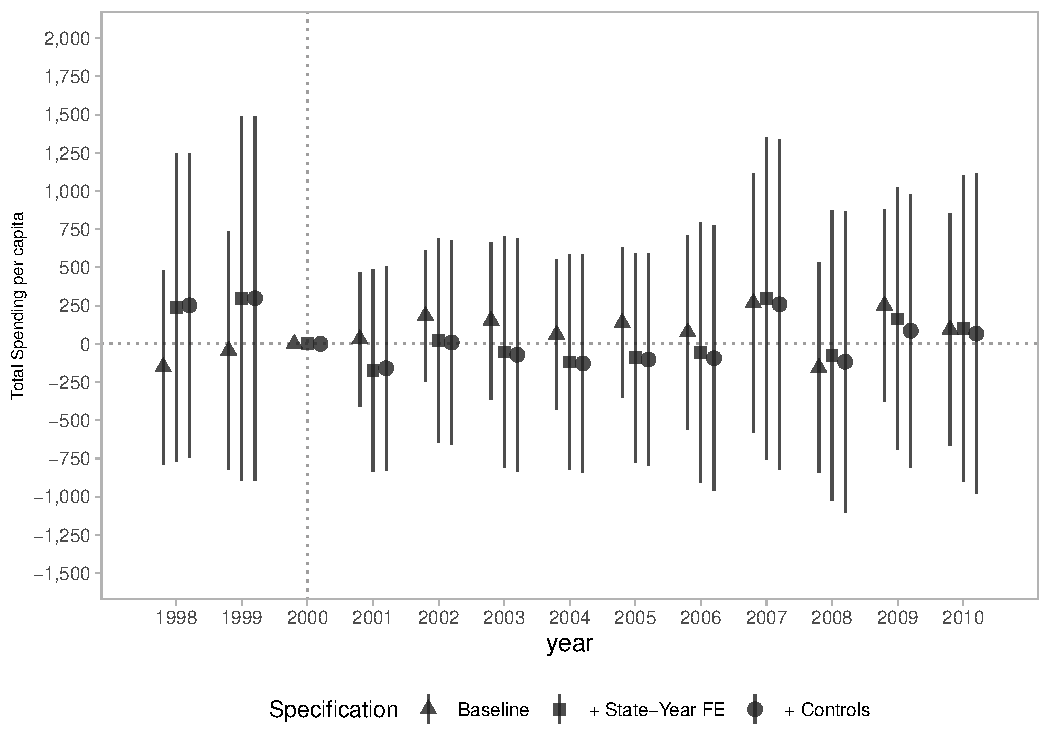
\includegraphics[width=\textwidth]{plots/spending/finbra_desp_o_pcapita_dist_ec29_baseline_dist_ec29_baseline_full.pdf}
    \end{subfigure}
    \begin{subfigure}{0.49\textwidth}
        \centering
        \caption{\scriptsize Human Resource Spending}\label{fig:finbra1_b}
        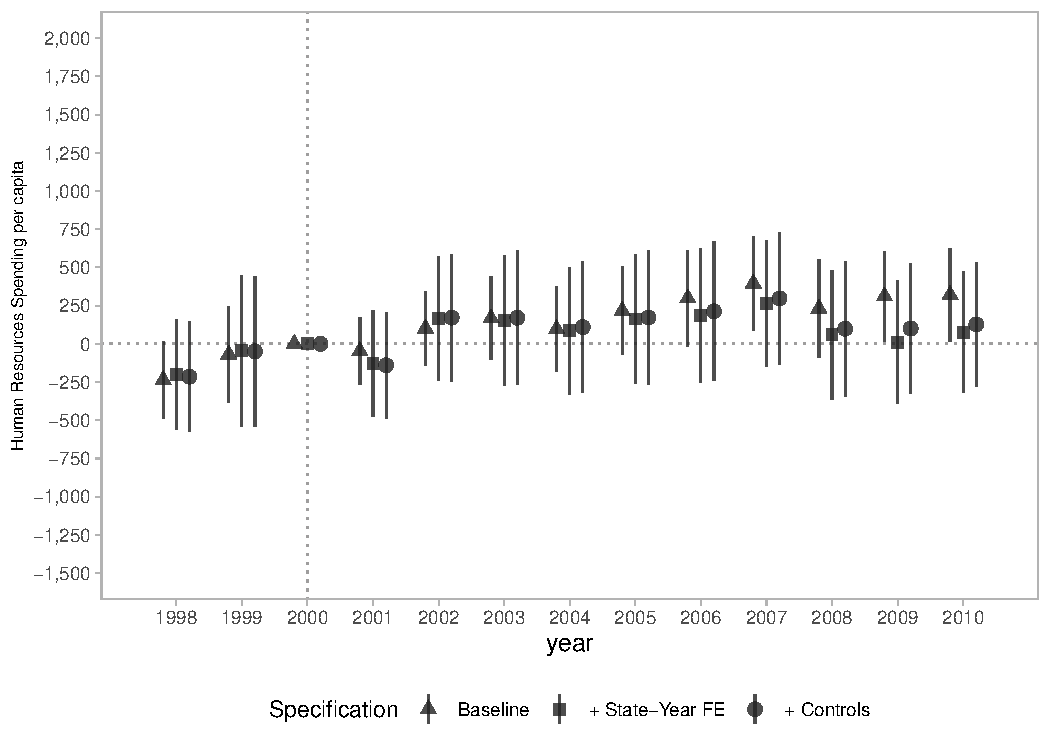
\includegraphics[width=\textwidth]{plots/spending/finbra_desp_pessoal_pcapita_dist_ec29_baseline_dist_ec29_baseline_full.pdf}
    \end{subfigure}
    \begin{subfigure}{0.49\textwidth}
        \centering
        \caption{\scriptsize Investment Spending}\label{fig:finbra1_c}
        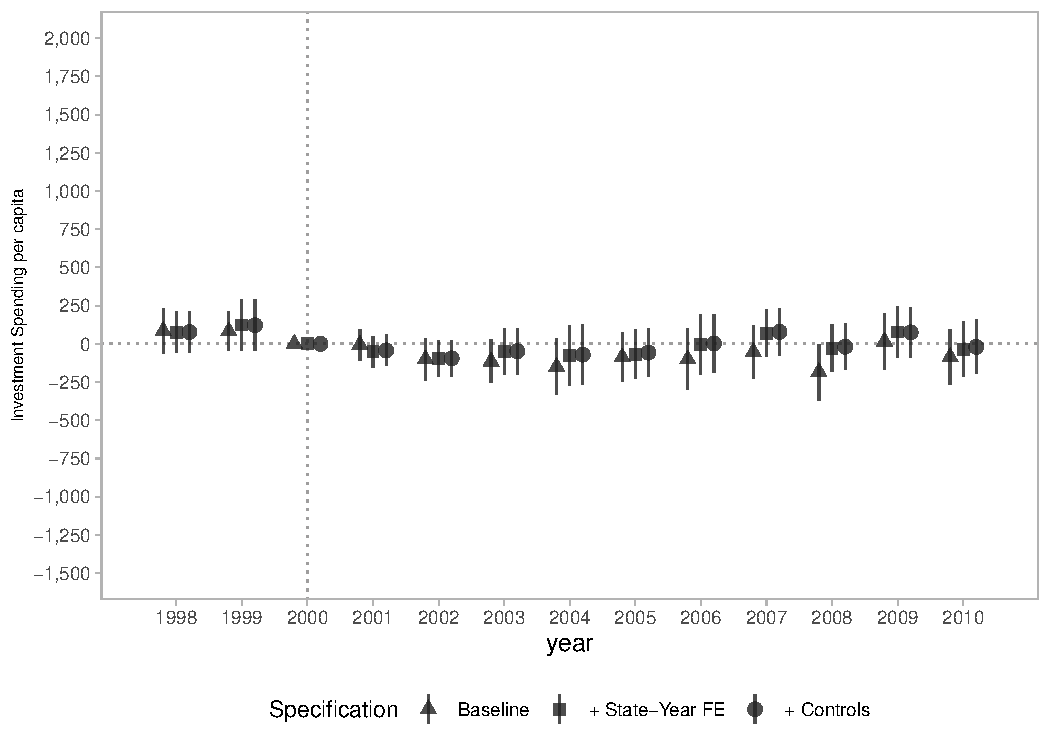
\includegraphics[width=\textwidth]{plots/spending/finbra_desp_investimento_pcapita_dist_ec29_baseline_dist_ec29_baseline_full.pdf}
    \end{subfigure}
    \begin{subfigure}{0.49\textwidth}
        \centering
        \caption{\scriptsize Other Spending}\label{fig:finbra1_d}
        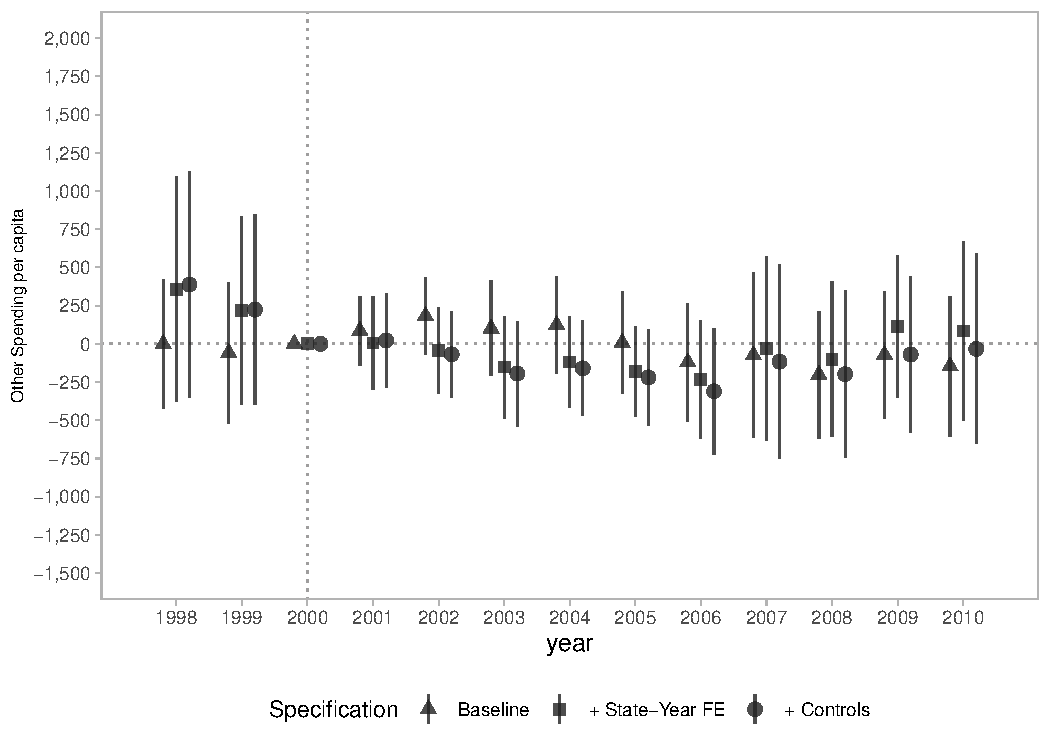
\includegraphics[width=\textwidth]{plots/spending/finbra_desp_outros_nature_pcapita_dist_ec29_baseline_dist_ec29_baseline_full.pdf}
    \end{subfigure}
    
    \end{center}
    
\end{figure}


\begin{figure}[h]
    \begin{center}
    \caption{Causal Effects on Public Spending (\% of Total Spending) - By Type}\label{fig:finbra2}
    \begin{subfigure}{0.32\textwidth}
        \centering
        \caption{\scriptsize Human Resource Spending}\label{fig:finbra2_a}
        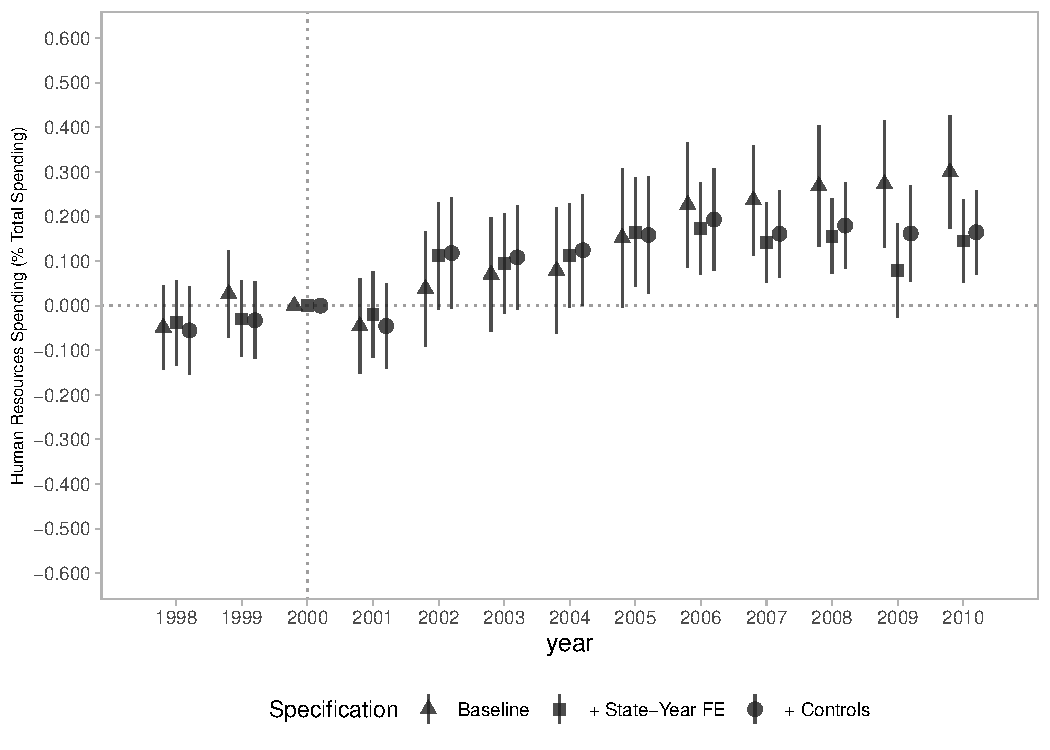
\includegraphics[width=\textwidth]{plots/spending/finbra_desp_pessoal_share_dist_ec29_baseline_dist_ec29_baseline_full.pdf}
    \end{subfigure}
    \begin{subfigure}{0.32\textwidth}
        \centering
        \caption{\scriptsize Investment Spending}\label{fig:finbra2_b}
        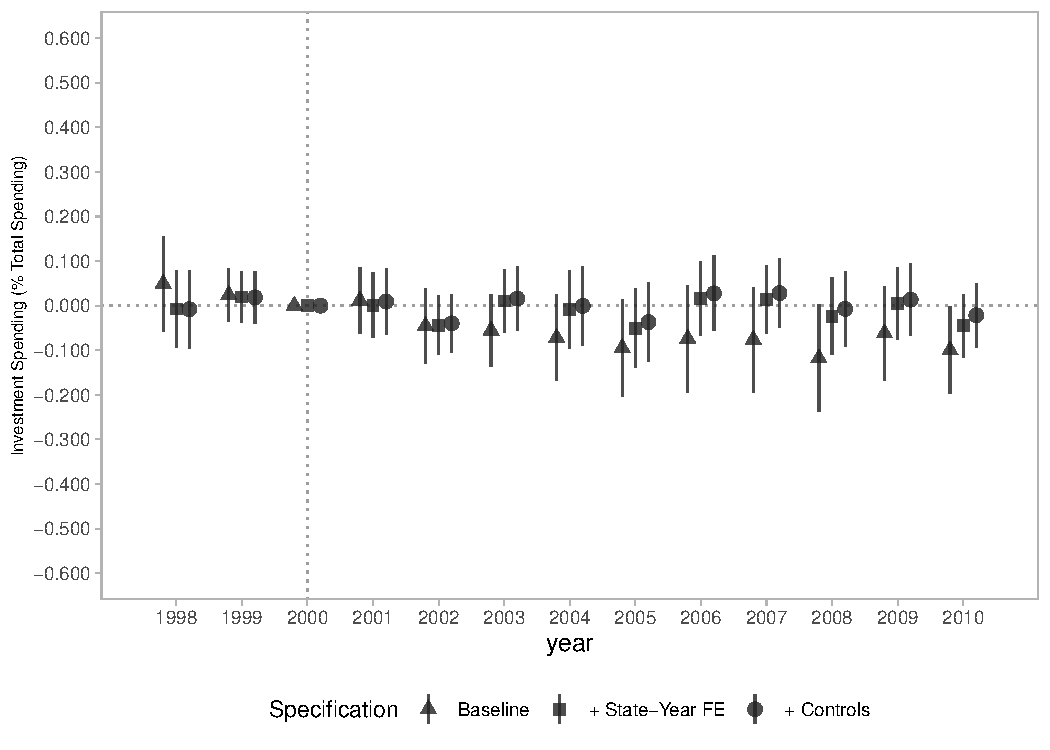
\includegraphics[width=\textwidth]{plots/spending/finbra_desp_investimento_share_dist_ec29_baseline_dist_ec29_baseline_full.pdf}
    \end{subfigure}
    \begin{subfigure}{0.32\textwidth}
        \centering
        \caption{\scriptsize Other Spending}\label{fig:finbra2_c}
        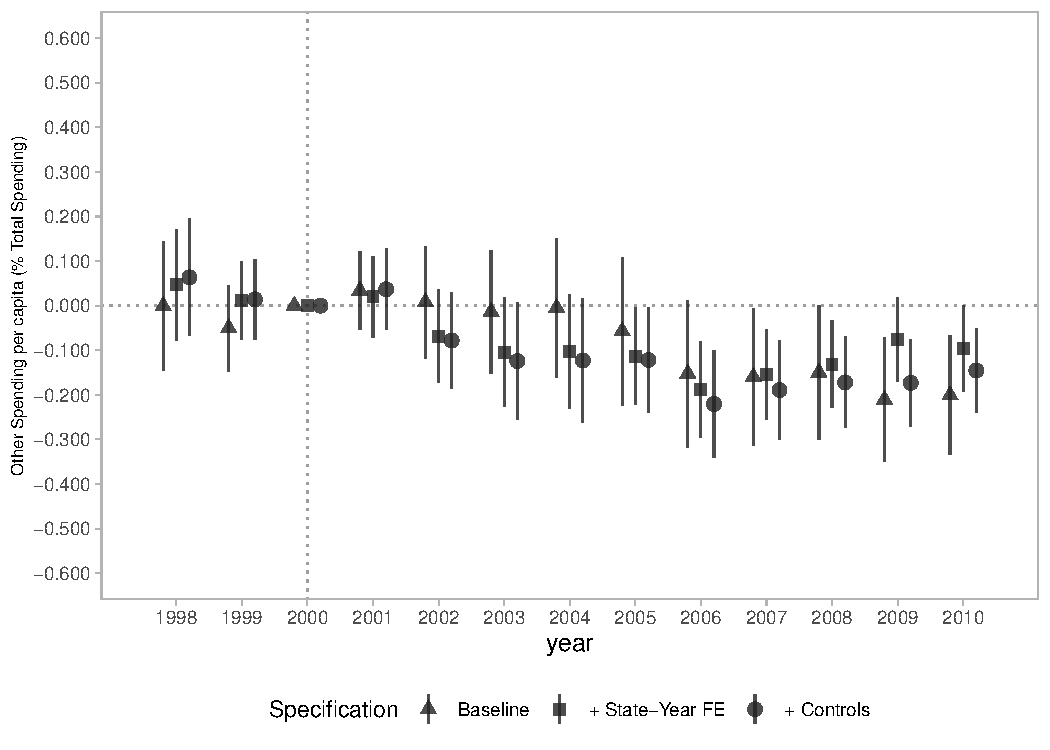
\includegraphics[width=\textwidth]{plots/spending/finbra_desp_outros_nature_share_dist_ec29_baseline_dist_ec29_baseline_full.pdf}
    \end{subfigure}
    
    \end{center}
    
\end{figure}




\begin{figure}[h]
    \begin{center}
    \caption{Causal Effects on Public Spending per capita - By Category}\label{fig:finbra3}
    \begin{subfigure}{0.32\textwidth}
        \caption{\scriptsize Health and Sanitation Spending}\label{fig:finbra3_a}
        \centering
        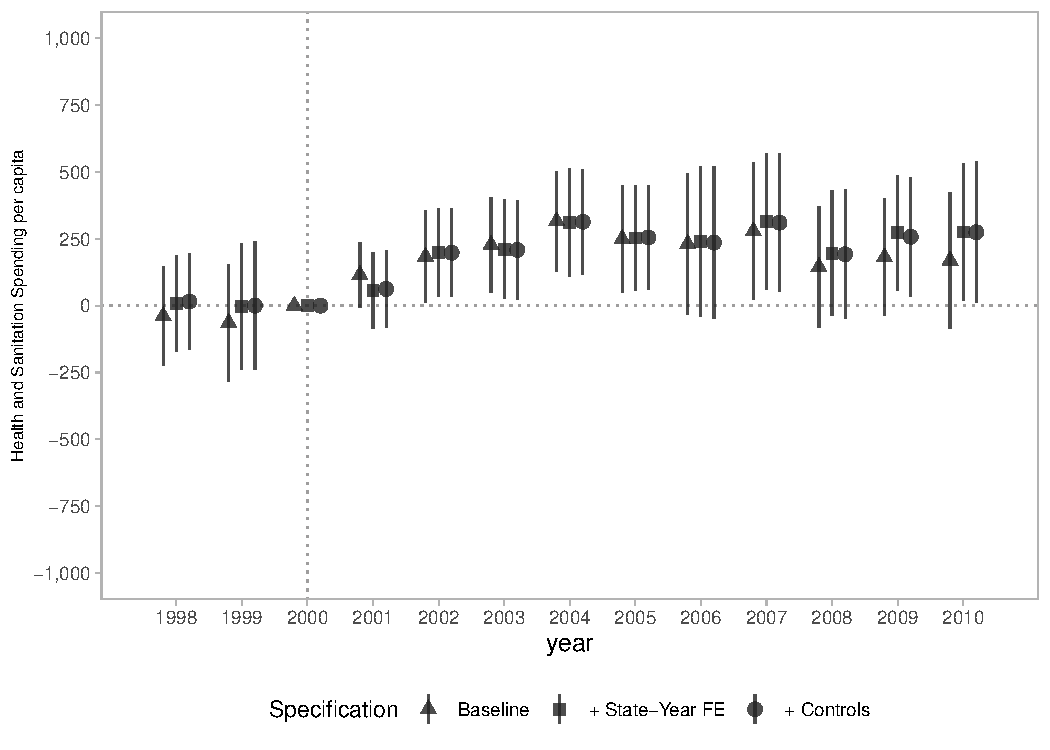
\includegraphics[width=\textwidth]{plots/spending/finbra_desp_saude_san_pcapita_dist_ec29_baseline_dist_ec29_baseline_full.pdf}
    \end{subfigure}
    \begin{subfigure}{0.32\textwidth}
        \centering
        \caption{\scriptsize Transport Spending}\label{fig:finbra3_b}
        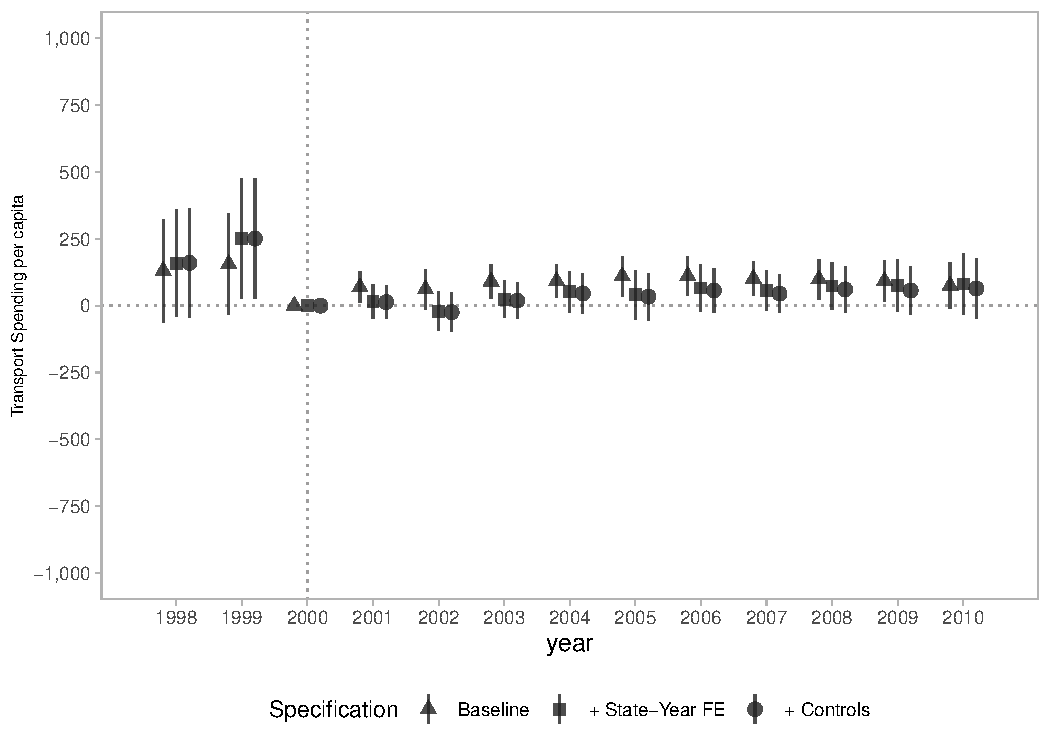
\includegraphics[width=\textwidth]{plots/spending/finbra_desp_transporte_pcapita_dist_ec29_baseline_dist_ec29_baseline_full.pdf}
    \end{subfigure}
    \begin{subfigure}{0.32\textwidth}
        \centering
        \caption{\scriptsize Education and Culture Spending}\label{fig:finbra3_c}
        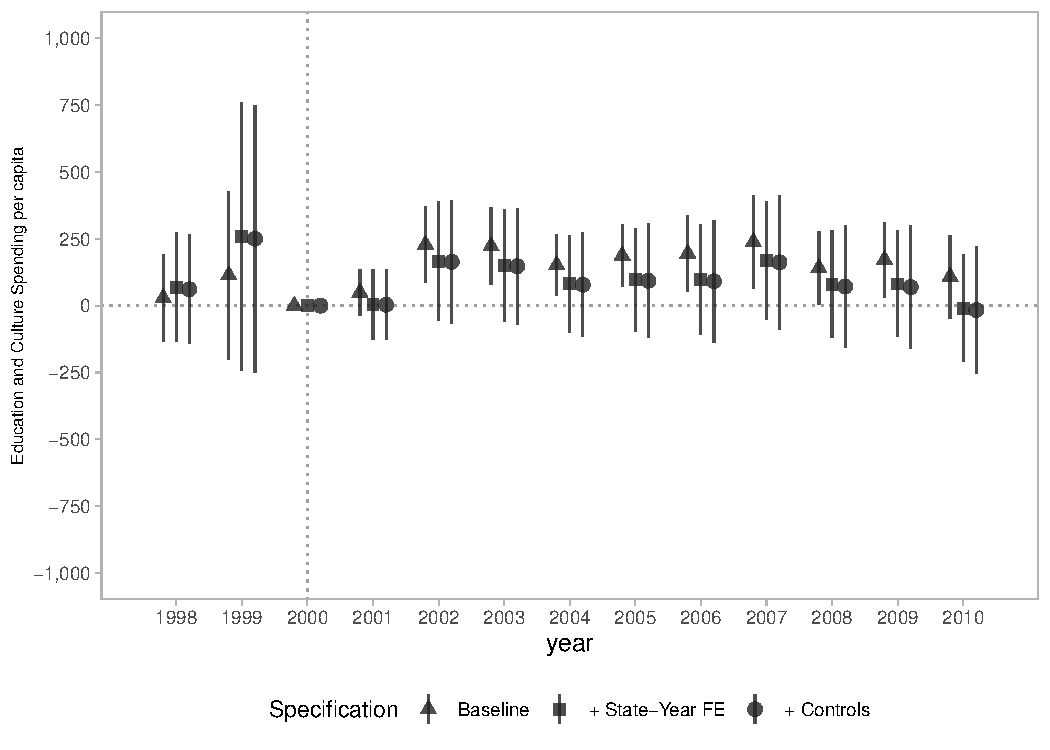
\includegraphics[width=\textwidth]{plots/spending/finbra_desp_educ_cultura_pcapita_dist_ec29_baseline_dist_ec29_baseline_full.pdf}
    \end{subfigure}
    \begin{subfigure}{0.32\textwidth}
        \centering
        \caption{\scriptsize Housing and Urban Spending}\label{fig:finbr3_d}
        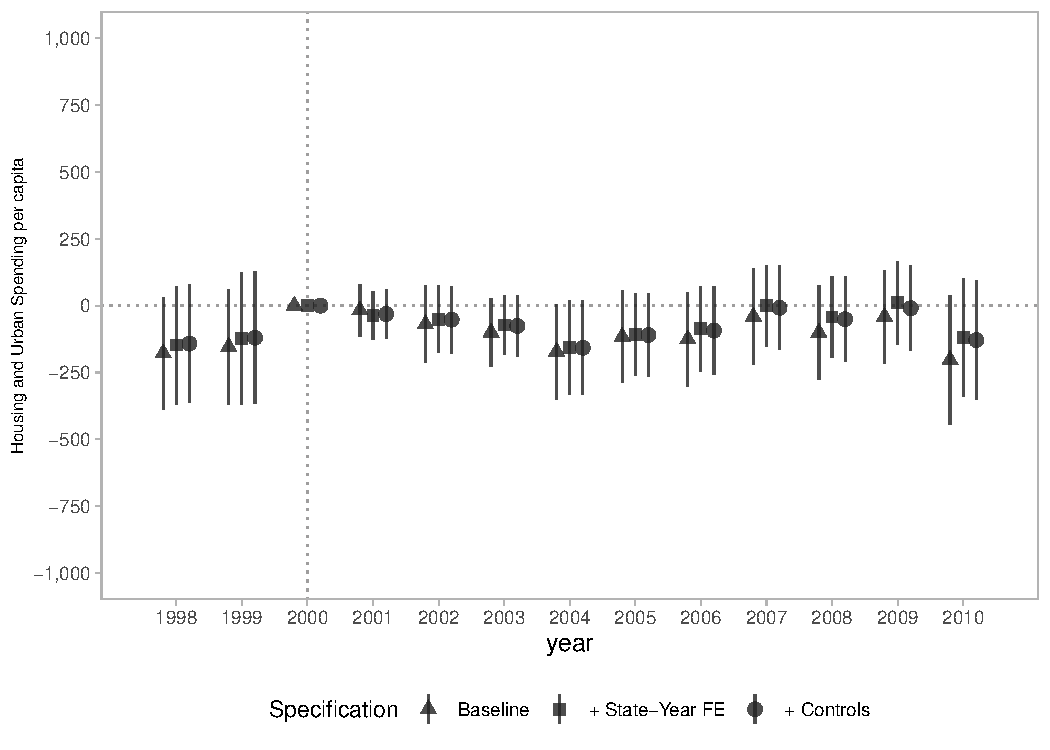
\includegraphics[width=\textwidth]{plots/spending/finbra_desp_hab_urb_pcapita_dist_ec29_baseline_dist_ec29_baseline_full.pdf}
    \end{subfigure}
    \begin{subfigure}{0.32\textwidth}
        \centering
        \caption{\scriptsize Social Assistance Spending}\label{fig:finbra3_e}
        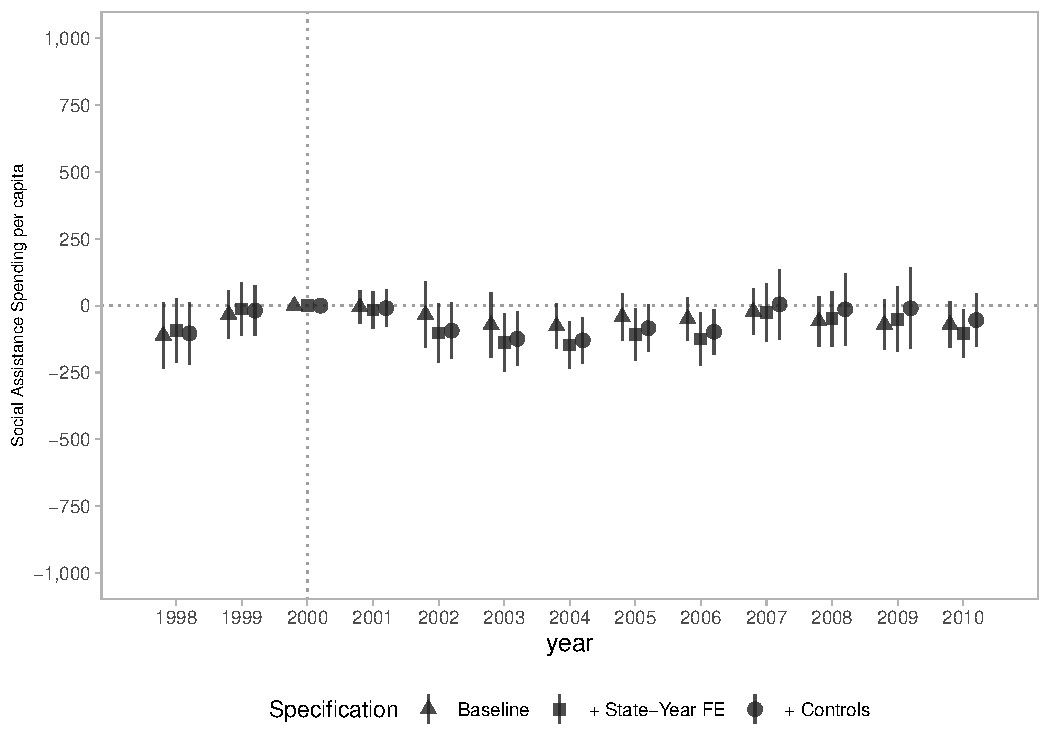
\includegraphics[width=\textwidth]{plots/spending/finbra_desp_assist_prev_pcapita_dist_ec29_baseline_dist_ec29_baseline_full.pdf}
    \end{subfigure}
    \begin{subfigure}{0.32\textwidth}
        \centering
        \caption{\scriptsize Spending in Other Categories}\label{fig:finbra3_f}
        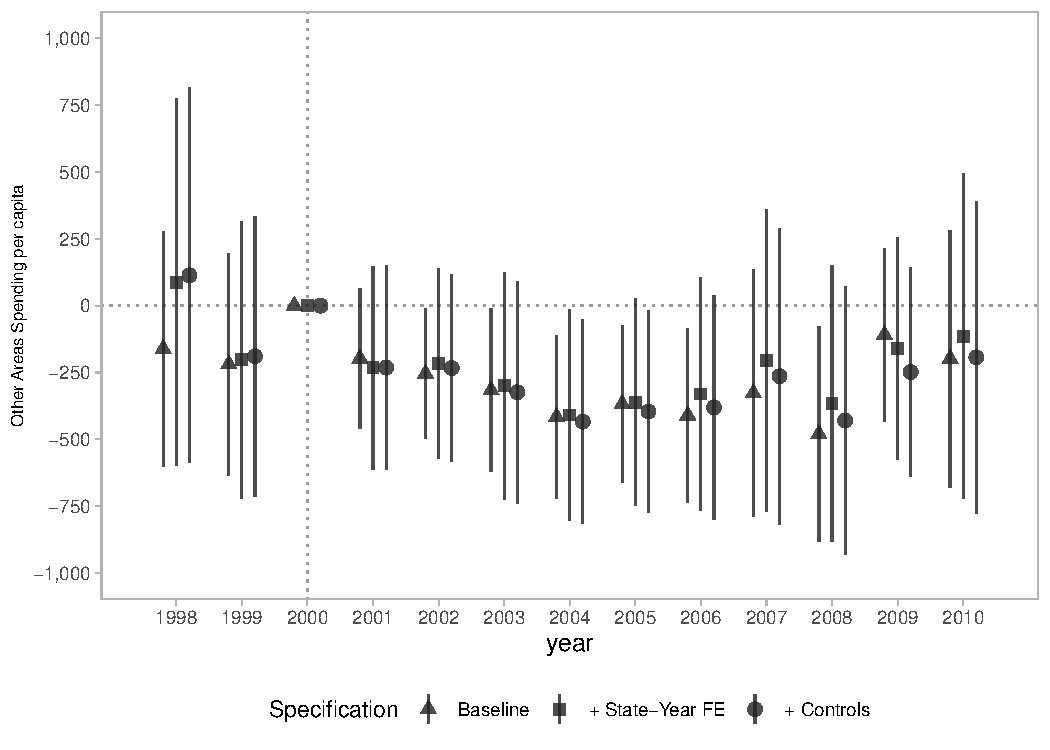
\includegraphics[width=\textwidth]{plots/spending/finbra_desp_outros_area_pcapita_dist_ec29_baseline_dist_ec29_baseline_full.pdf}
    \end{subfigure}
    
    \end{center}
    
\end{figure}



\begin{figure}[h]
    \begin{center}
    \caption{Causal Effects on Public Spending (\% of Total Spending) - By Category}\label{fig:finbra4}
    \begin{subfigure}{0.32\textwidth}
        \caption{\scriptsize Health and Sanitation Spending}\label{fig:finbra4_a}
        \centering
        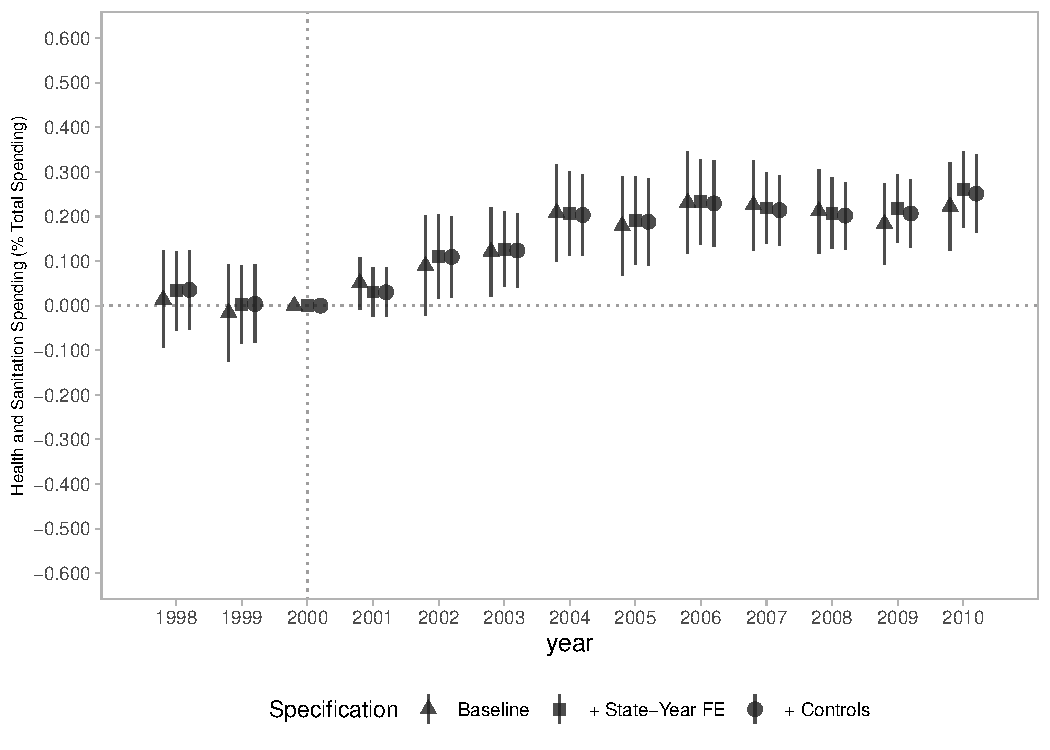
\includegraphics[width=\textwidth]{plots/spending/finbra_desp_saude_san_share_dist_ec29_baseline_dist_ec29_baseline_full.pdf}
    \end{subfigure}
    \begin{subfigure}{0.32\textwidth}
        \centering
        \caption{\scriptsize Transport Spending}\label{fig:finbra4_b}
        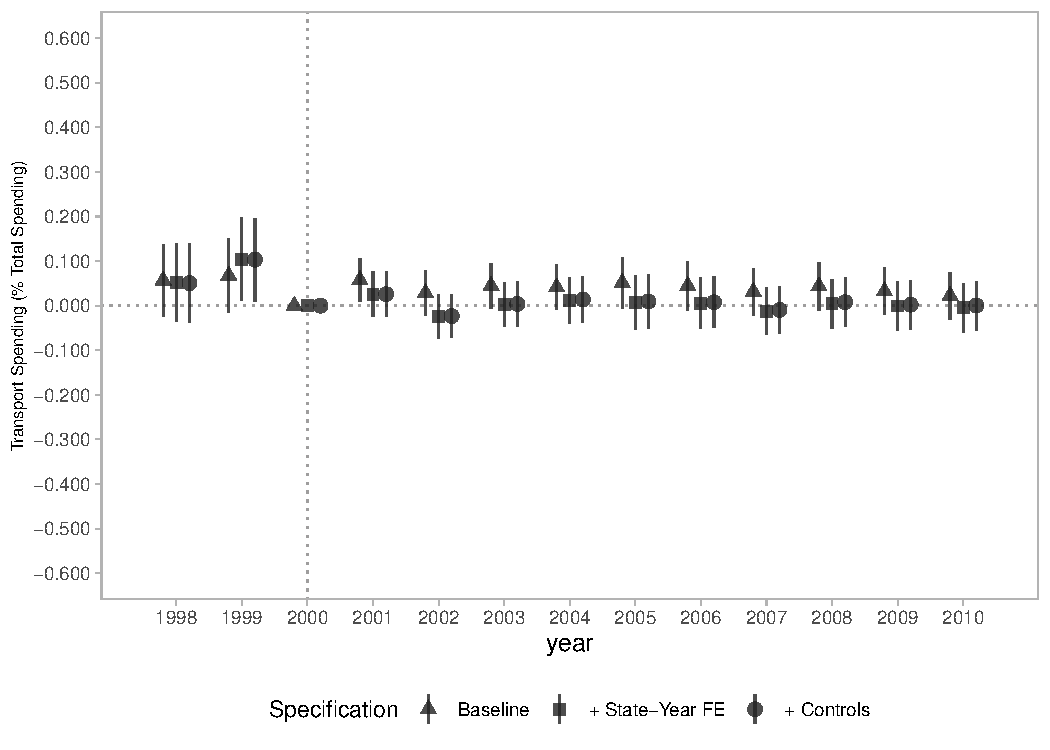
\includegraphics[width=\textwidth]{plots/spending/finbra_desp_transporte_share_dist_ec29_baseline_dist_ec29_baseline_full.pdf}
    \end{subfigure}
    \begin{subfigure}{0.32\textwidth}
        \centering
        \caption{\scriptsize Education and Culture Spending}\label{fig:finbra4_c}
        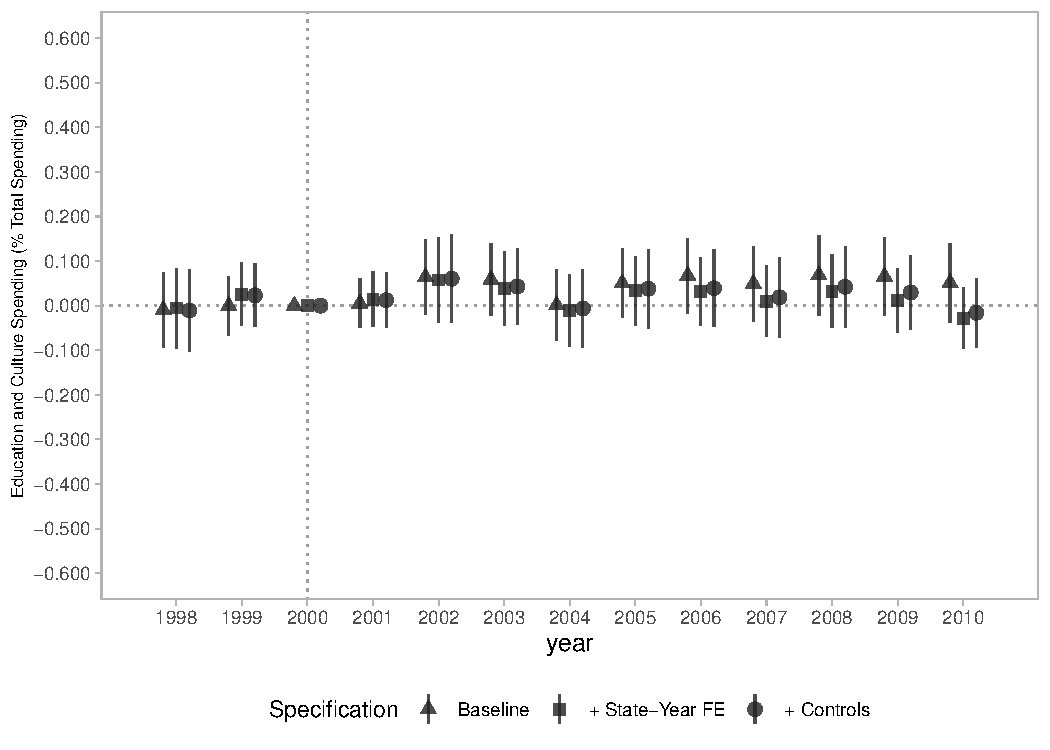
\includegraphics[width=\textwidth]{plots/spending/finbra_desp_educ_cultura_share_dist_ec29_baseline_dist_ec29_baseline_full.pdf}
    \end{subfigure}
    \begin{subfigure}{0.32\textwidth}
        \centering
        \caption{\scriptsize Housing and Urban Spending}\label{fig:finbr4_d}
        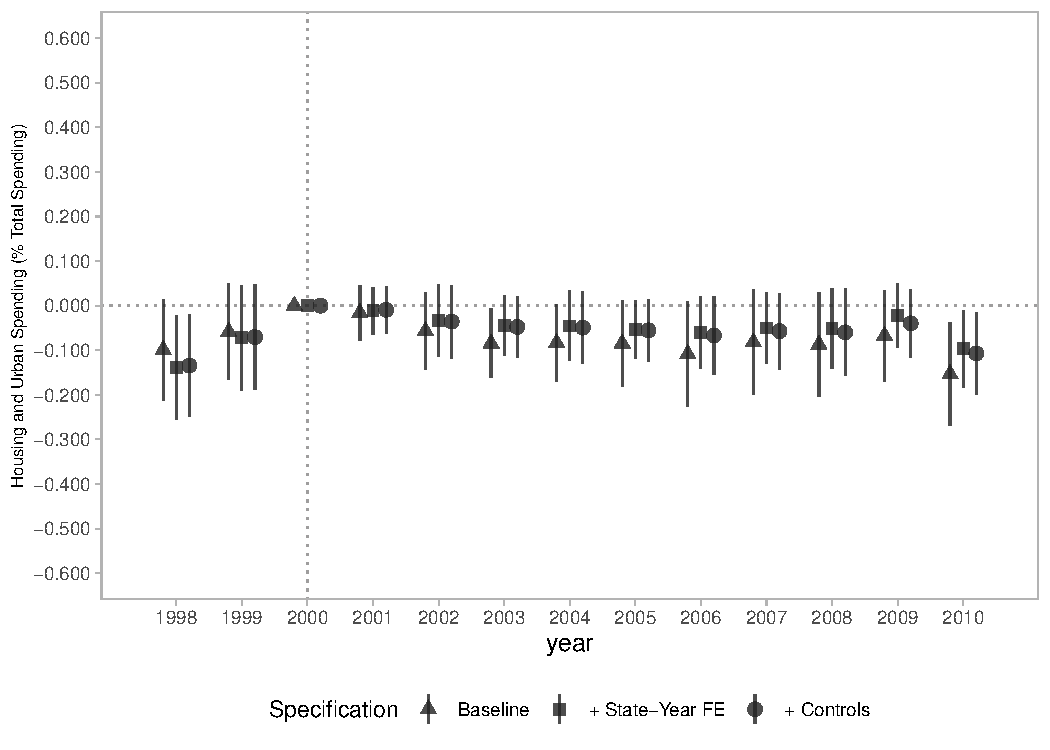
\includegraphics[width=\textwidth]{plots/spending/finbra_desp_hab_urb_share_dist_ec29_baseline_dist_ec29_baseline_full.pdf}
    \end{subfigure}
    \begin{subfigure}{0.32\textwidth}
        \centering
        \caption{\scriptsize Social Assistance Spending}\label{fig:finbra4_e}
        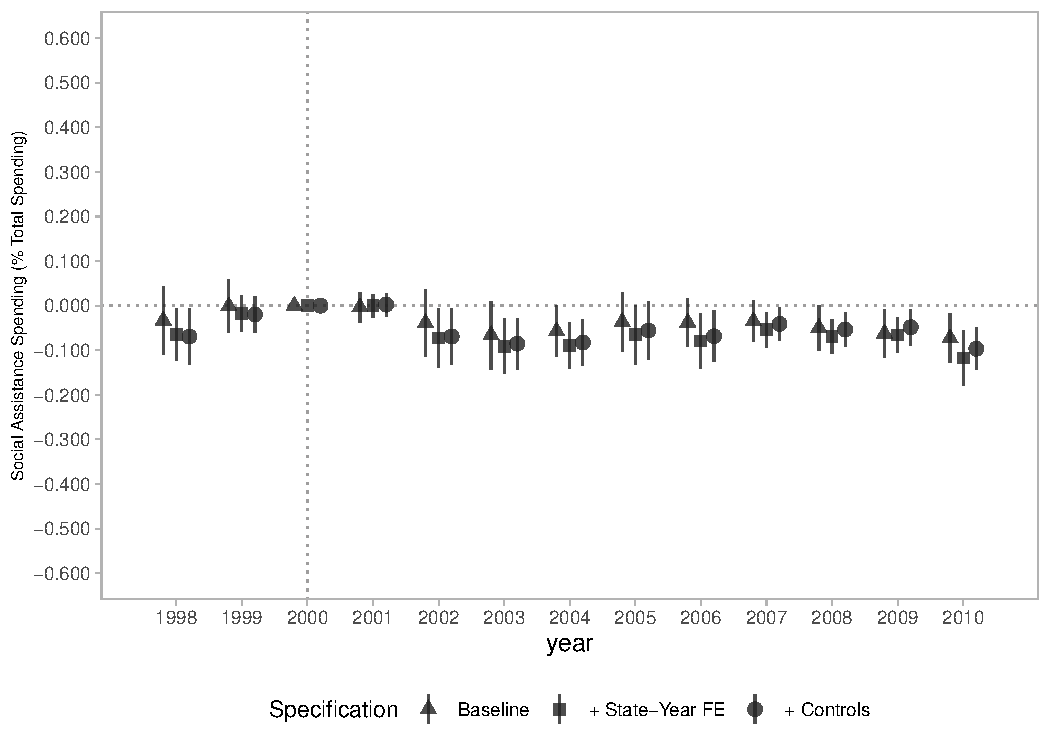
\includegraphics[width=\textwidth]{plots/spending/finbra_desp_assist_prev_share_dist_ec29_baseline_dist_ec29_baseline_full.pdf}
    \end{subfigure}
    \begin{subfigure}{0.32\textwidth}
        \centering
        \caption{\scriptsize Spending in Other Categories}\label{fig:finbra4_f}
        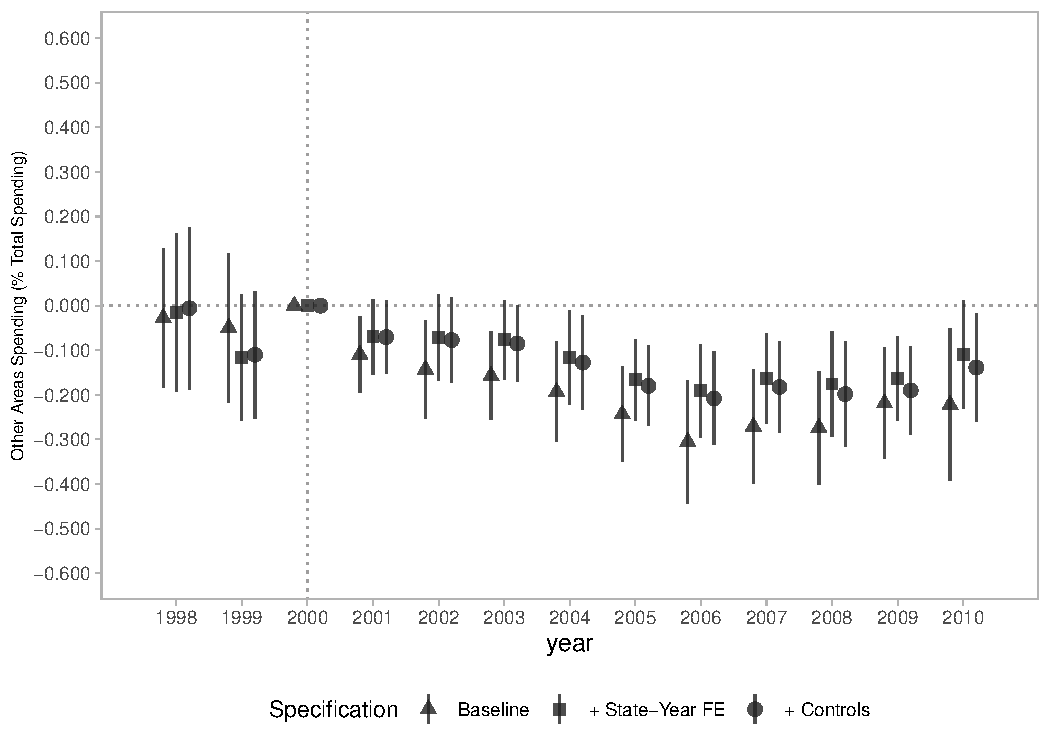
\includegraphics[width=\textwidth]{plots/spending/finbra_desp_outros_area_share_dist_ec29_baseline_dist_ec29_baseline_full.pdf}
    \end{subfigure}
    
    \end{center}
    
\end{figure}


\begin{figure}[h]
    \begin{center}
    \caption{Causal Effects on Public Health Spending per capita - By Source}\label{fig:siops1}
    \begin{subfigure}{0.32\textwidth}
        \caption{\scriptsize Total Health Spending}\label{fig:siops1_a}
        \centering
        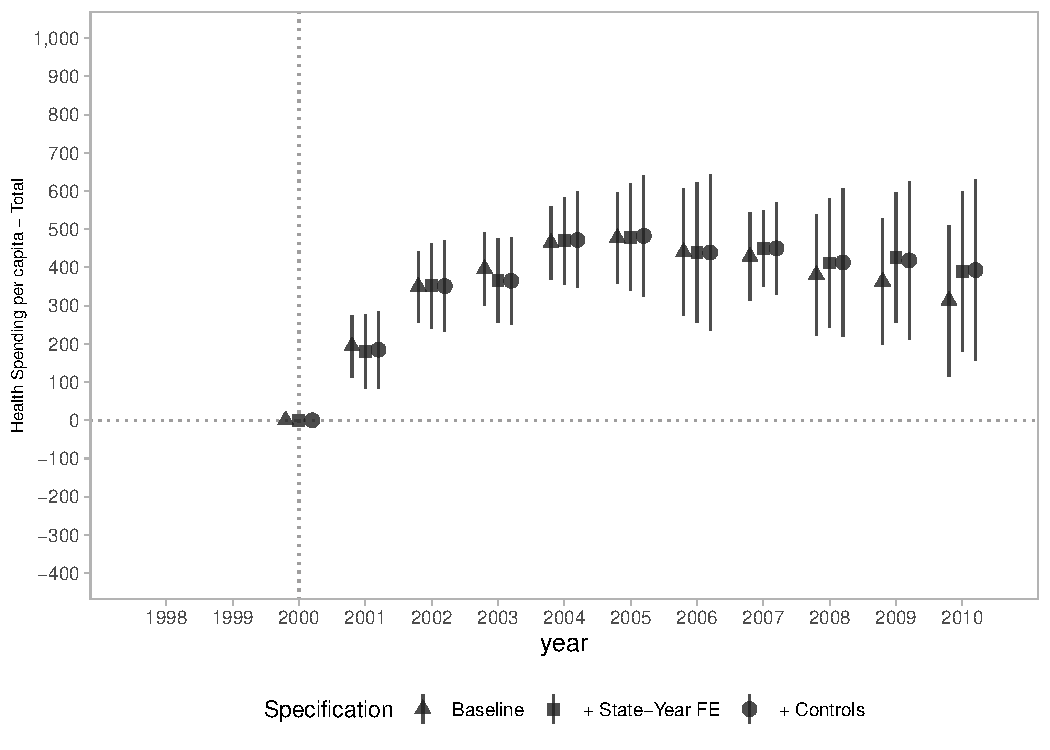
\includegraphics[width=\textwidth]{plots/spending/siops_despsaude_pcapita_dist_ec29_baseline_dist_ec29_baseline_full.pdf}
    \end{subfigure}
    \begin{subfigure}{0.32\textwidth}
        \centering
        \caption{\scriptsize Own Resources}\label{fig:siops1_b}
        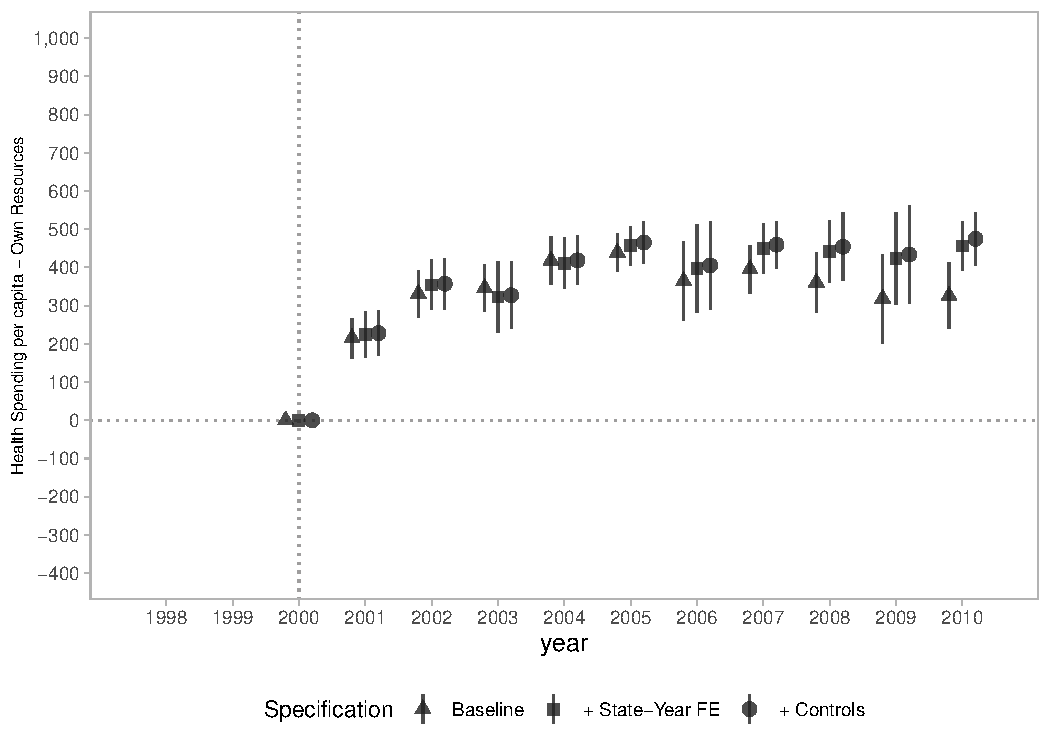
\includegraphics[width=\textwidth]{plots/spending/siops_desprecpropriosaude_pcapita_dist_ec29_baseline_dist_ec29_baseline_full.pdf}
    \end{subfigure}
    \begin{subfigure}{0.32\textwidth}
        \centering
        \caption{\scriptsize Transfers}\label{fig:siops1_c}
        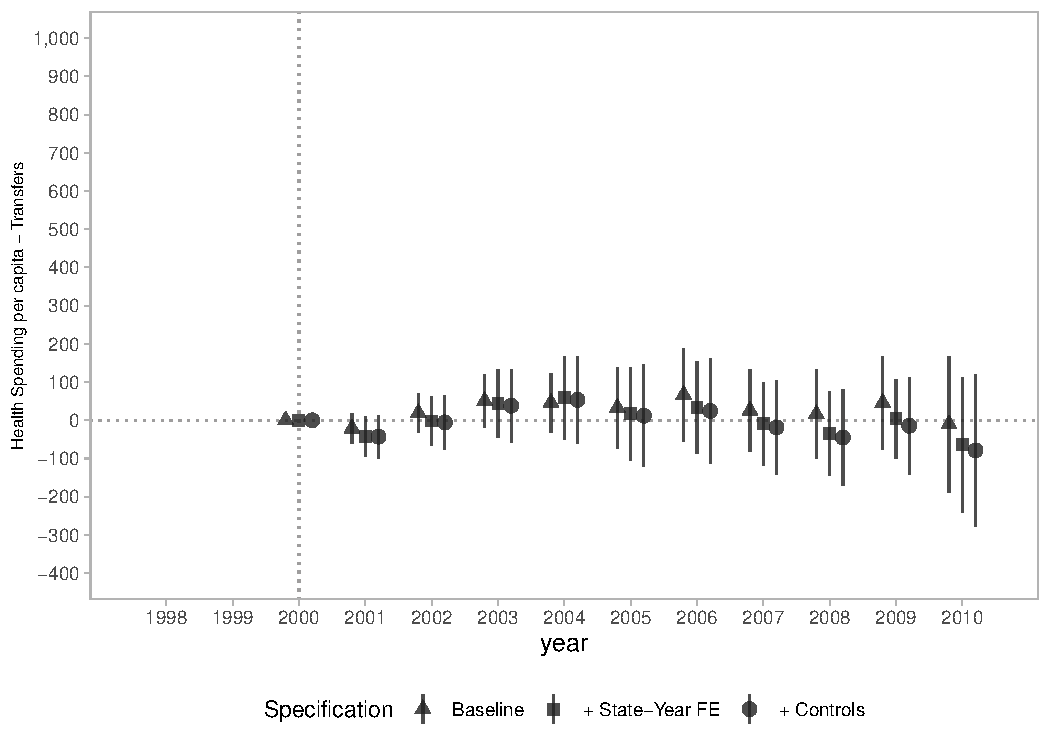
\includegraphics[width=\textwidth]{plots/spending/siops_despexrecproprio_pcapita_dist_ec29_baseline_dist_ec29_baseline_full.pdf}
    \end{subfigure}
    
    \end{center}
    
\end{figure}

\begin{figure}[h]
    \begin{center}
    \caption{Causal Effects on Public Health Spending (\% of Total Health Spending) - By Source}\label{fig:siops2}
    \begin{subfigure}{0.48\textwidth}
        \centering
        \caption{\scriptsize Own Resources}\label{fig:siops2_a}
        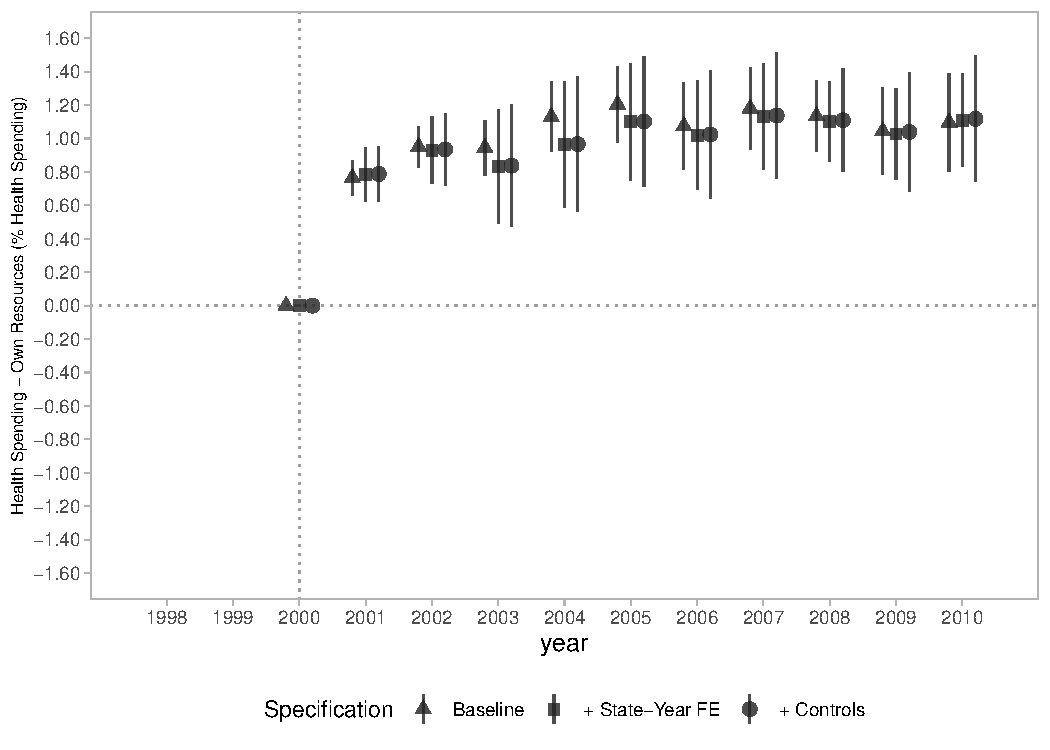
\includegraphics[width=\textwidth]{plots/spending/siops_desprecpropriosaude_share_dist_ec29_baseline_dist_ec29_baseline_full.pdf}
    \end{subfigure}
    \begin{subfigure}{0.48\textwidth}
        \centering
        \caption{\scriptsize Transfers}\label{fig:siops2_b}
        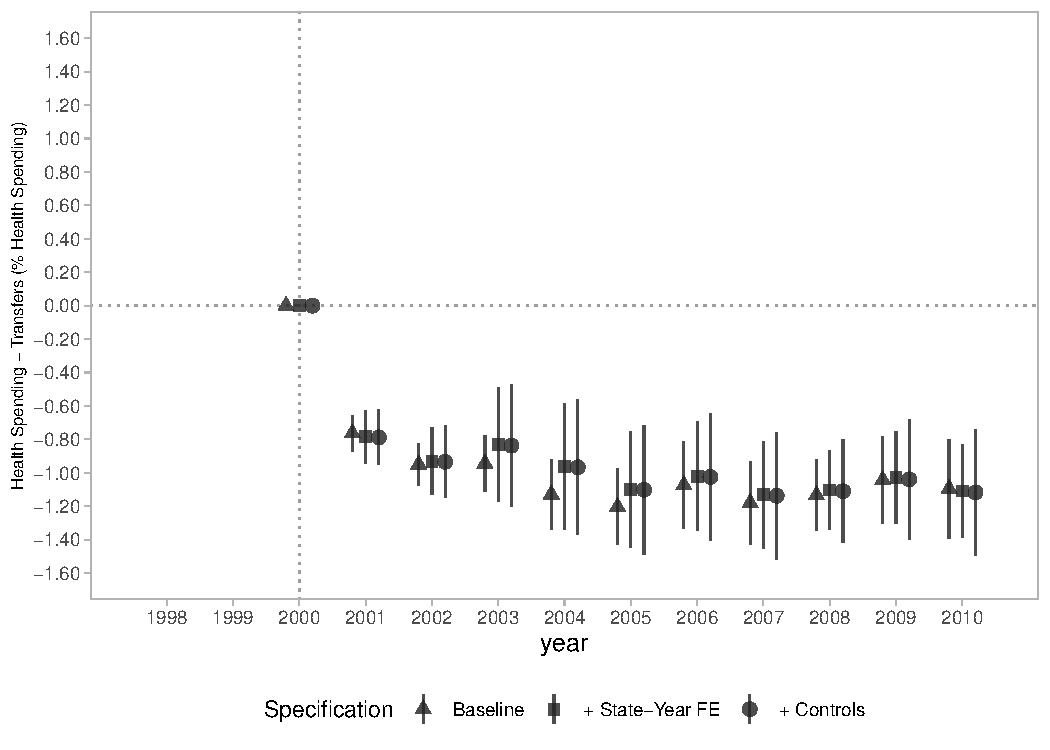
\includegraphics[width=\textwidth]{plots/spending/siops_despexrecproprio_share_dist_ec29_baseline_dist_ec29_baseline_full.pdf}
    \end{subfigure}
    
    \end{center}
    
\end{figure}

\begin{figure}[h]
    \begin{center}
    \caption{Causal Effects on Public Health Spending per capita - By Type}\label{fig:siops3}
    \begin{subfigure}{0.48\textwidth}
        \centering
        \caption{\scriptsize Human Resources}\label{fig:siops3_a}
        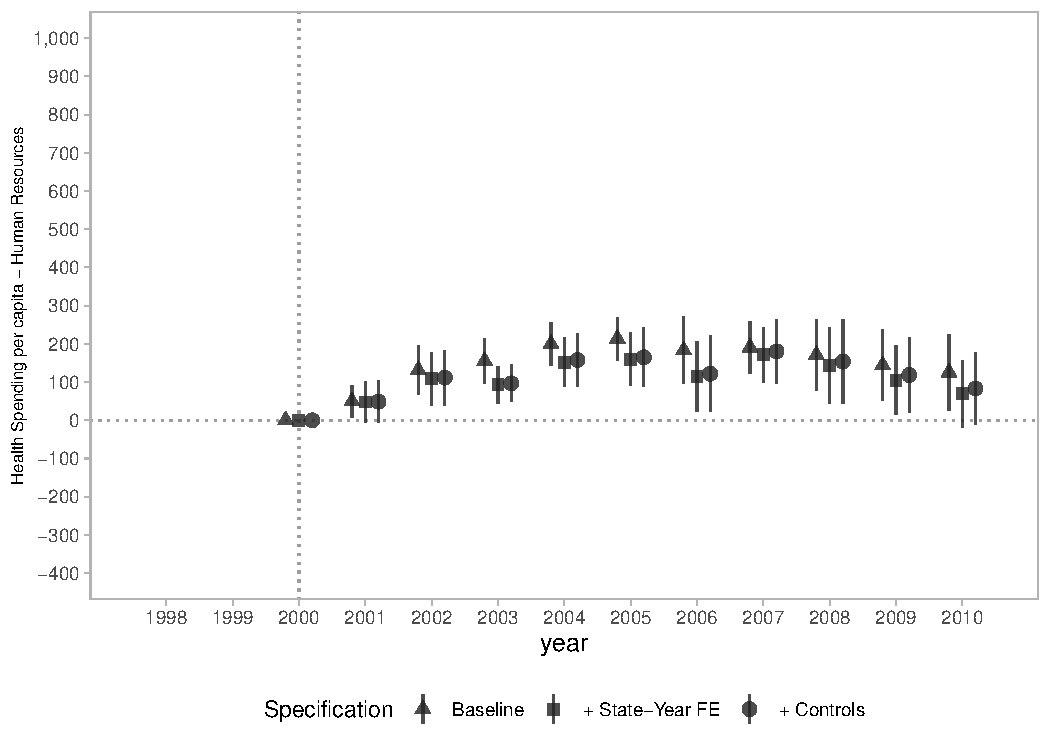
\includegraphics[width=\textwidth]{plots/spending/siops_desppessoal_pcapita_dist_ec29_baseline_dist_ec29_baseline_full.pdf}
    \end{subfigure}
    \begin{subfigure}{0.48\textwidth}
        \centering
        \caption{\scriptsize Investiment}\label{fig:siops3_b}
        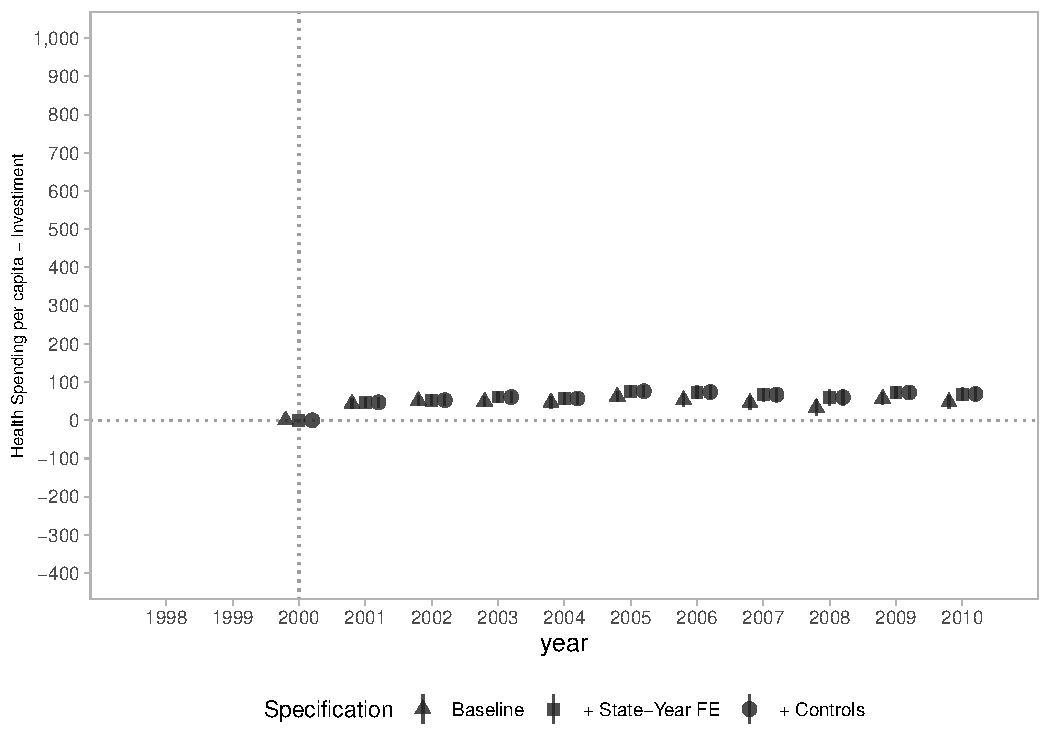
\includegraphics[width=\textwidth]{plots/spending/siops_despinvest_pcapita_dist_ec29_baseline_dist_ec29_baseline_full.pdf}
    \end{subfigure}
    \begin{subfigure}{0.48\textwidth}
        \centering
        \caption{\scriptsize 3rd parties services}\label{fig:siops3_c}
        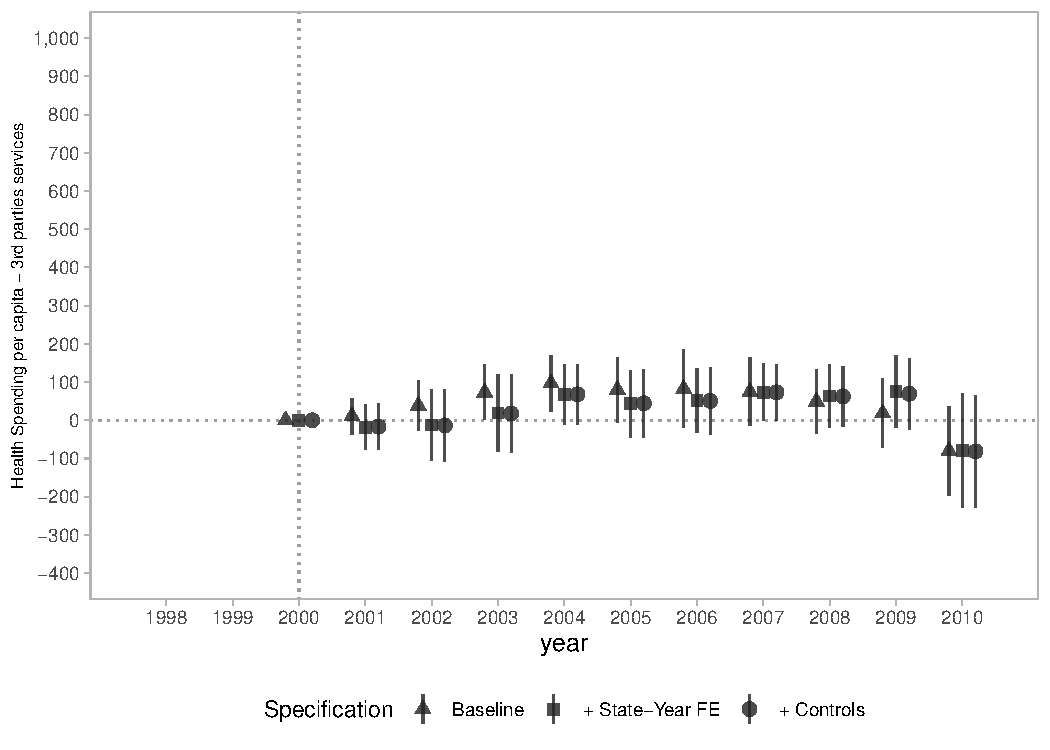
\includegraphics[width=\textwidth]{plots/spending/siops_despservicoster_pcapita_dist_ec29_baseline_dist_ec29_baseline_full.pdf}
    \end{subfigure}
    \begin{subfigure}{0.48\textwidth}
        \centering
        \caption{\scriptsize Other Expenditures}\label{fig:siops3_d}
        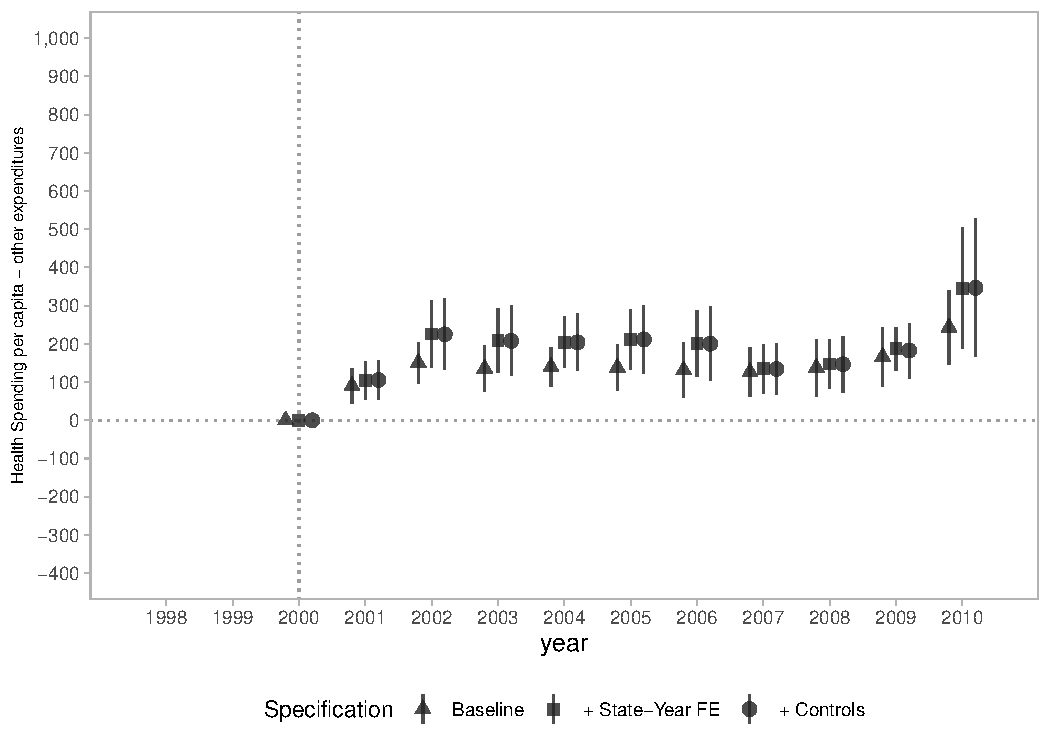
\includegraphics[width=\textwidth]{plots/spending/siops_despoutros_pcapita_dist_ec29_baseline_dist_ec29_baseline_full.pdf}
    \end{subfigure}
    
    \end{center}
    
\end{figure}

\begin{figure}[h]
    \begin{center}
    \caption{Causal Effects on Public Health Spending (\% of Total Health Spending) - By Type}\label{fig:siops4}
    \begin{subfigure}{0.48\textwidth}
        \centering
        \caption{\scriptsize Human Resources}\label{fig:siops4_a}
        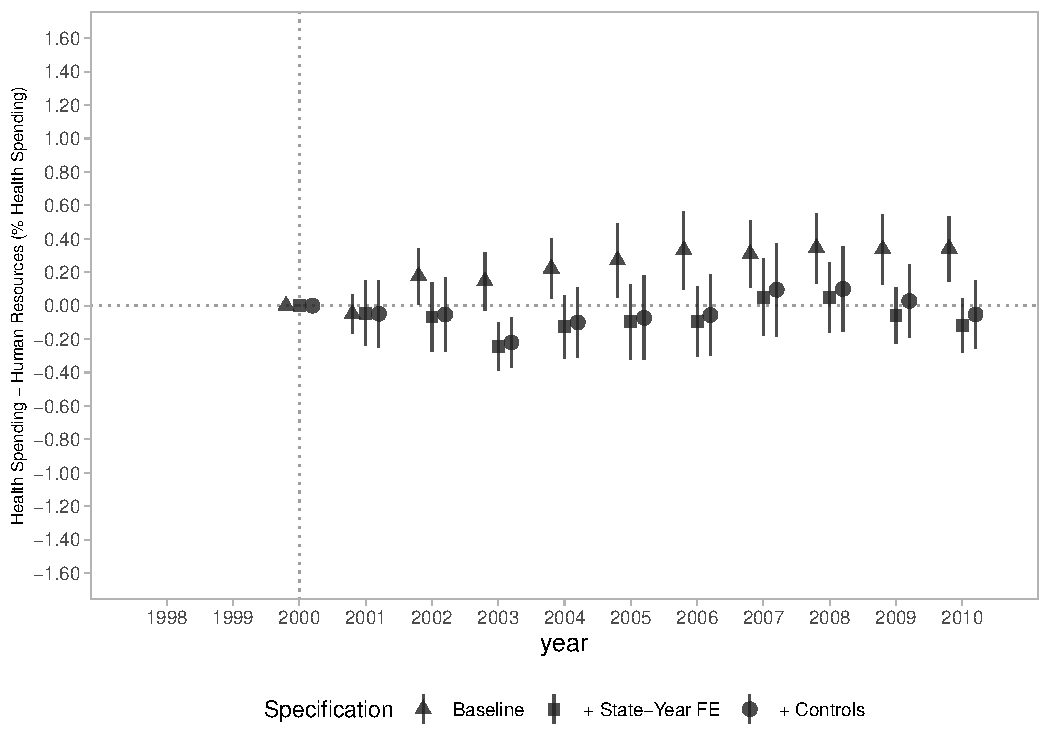
\includegraphics[width=\textwidth]{plots/spending/siops_desppessoal_share_dist_ec29_baseline_dist_ec29_baseline_full.pdf}
    \end{subfigure}
    \begin{subfigure}{0.48\textwidth}
        \centering
        \caption{\scriptsize Investiment}\label{fig:siops4_b}
        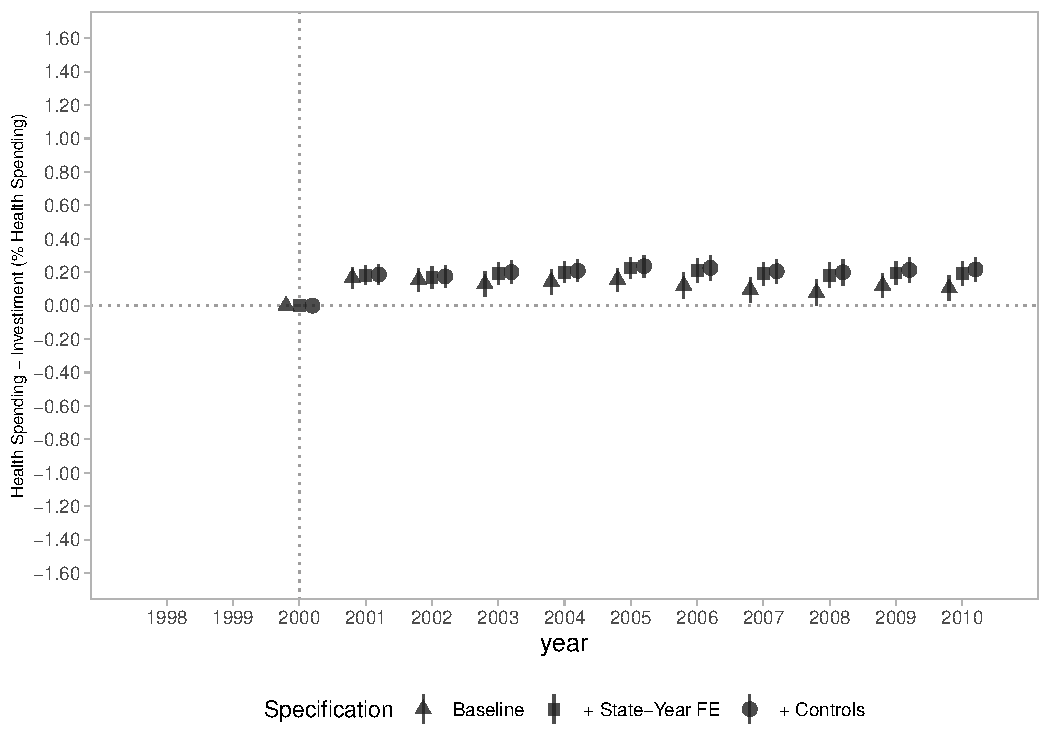
\includegraphics[width=\textwidth]{plots/spending/siops_despinvest_share_dist_ec29_baseline_dist_ec29_baseline_full.pdf}
    \end{subfigure}
    \begin{subfigure}{0.48\textwidth}
        \centering
        \caption{\scriptsize 3rd parties services}\label{fig:siops4_c}
        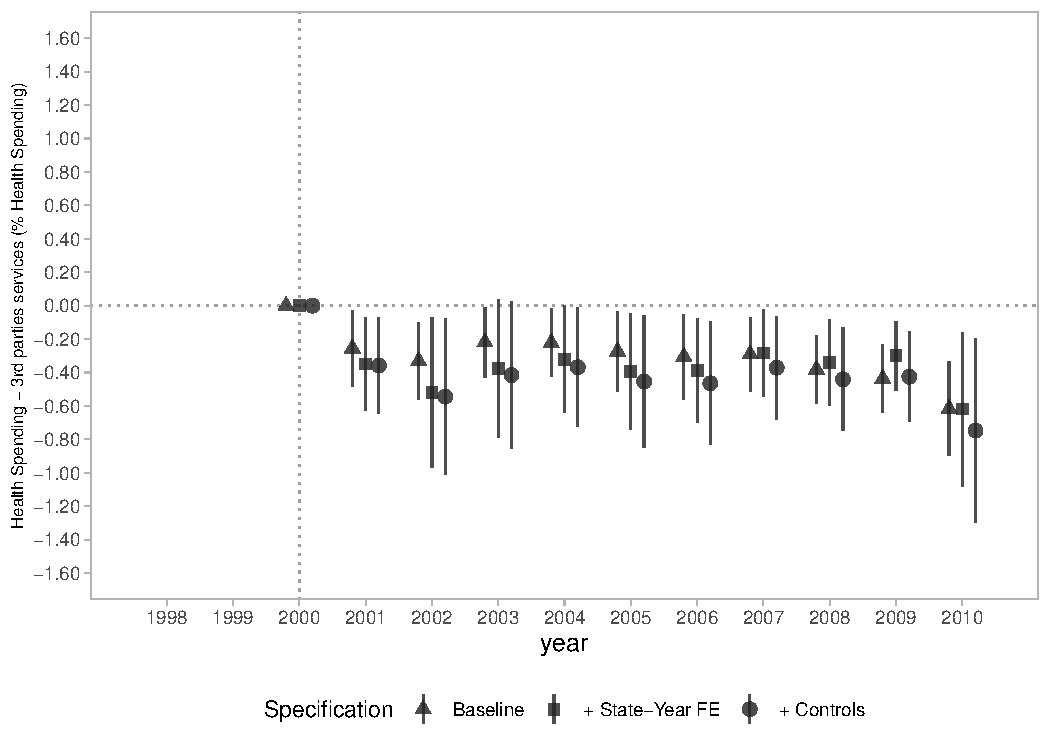
\includegraphics[width=\textwidth]{plots/spending/siops_despservicoster_share_dist_ec29_baseline_dist_ec29_baseline_full.pdf}
    \end{subfigure}
    \begin{subfigure}{0.48\textwidth}
        \centering
        \caption{\scriptsize Other Expenditures}\label{fig:siops4_d}
        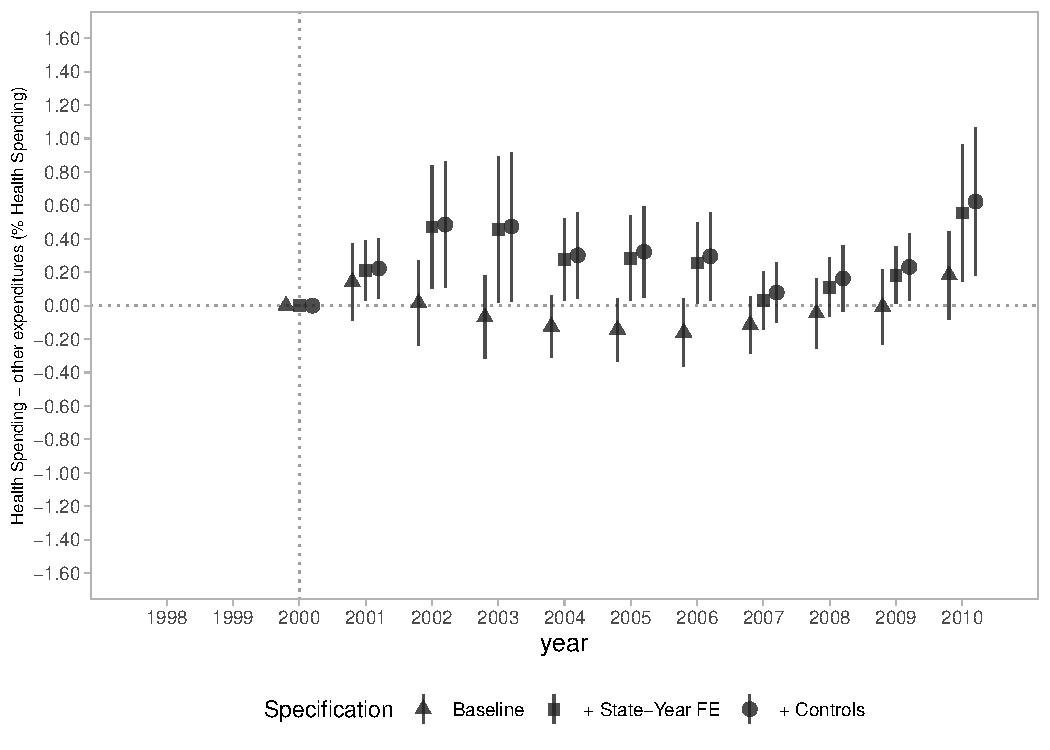
\includegraphics[width=\textwidth]{plots/spending/siops_despoutros_share_dist_ec29_baseline_dist_ec29_baseline_full.pdf}
    \end{subfigure}
    
    \end{center}
    
\end{figure}

\subsection{Causal Effects on Infant Mortality}

\begin{table}[H]
\begin{footnotesize}
\begin{center}
\scalebox{1}{
\begin{threeparttable}[b]

  \centering
  \caption{Causal Effects on Infant Mortality Rates}
    \begin{tabular}{rrrrrr}
          &       &       &       &       &  \\
    \midrule
    \midrule
          &       & \multicolumn{4}{c}{Distance to EC9 target} \\
\cmidrule{3-6}          &       & \multicolumn{1}{c}{(1)} & \multicolumn{1}{c}{(2)} & \multicolumn{1}{c}{(3)} & \multicolumn{1}{c}{obs} \\
    \midrule
    \multicolumn{1}{p{15.145em}}{\textbf{Infant Mortality Rate}} &       &       &       &       &  \\
    \multicolumn{1}{l}{\multirow{2}[0]{*}{Total}} &       & \multicolumn{1}{l}{0.999} & \multicolumn{1}{l}{0.867} & \multicolumn{1}{l}{-2.035} & \multicolumn{1}{c}{     64,313 } \\
          &       & \multicolumn{1}{l}{(3.987)} & \multicolumn{1}{l}{(3.585)} & \multicolumn{1}{l}{(3.207)} &  \\
    \multicolumn{1}{l}{\multirow{2}[0]{*}{Amenable to Primary Care}} &       & \multicolumn{1}{l}{-1.74**} & \multicolumn{1}{l}{-0.117} & \multicolumn{1}{l}{-0.785} & \multicolumn{1}{c}{     64,306 } \\
          &       & \multicolumn{1}{l}{(0.701)} & \multicolumn{1}{l}{(0.607)} & \multicolumn{1}{l}{(0.54)} &  \\
    \multicolumn{1}{l}{\multirow{2}[0]{*}{Non-Amenable to Primary Care}} &       & \multicolumn{1}{l}{2.738} & \multicolumn{1}{l}{0.983} & \multicolumn{1}{l}{-1.253} & \multicolumn{1}{c}{     64,313 } \\
          &       & \multicolumn{1}{l}{(3.517)} & \multicolumn{1}{l}{(3.301)} & \multicolumn{1}{l}{(2.998)} &  \\
          &       &       &       &       &  \\
    \multicolumn{1}{p{15.145em}}{\textbf{By timing}} &       &       &       &       &  \\
    \multicolumn{1}{l}{\multirow{2}[0]{*}{Fetal}} &       & \multicolumn{1}{l}{-0.02**} & \multicolumn{1}{l}{-0.007} & \multicolumn{1}{l}{-0.007} & \multicolumn{1}{c}{     64,305 } \\
          &       & \multicolumn{1}{l}{(0.01)} & \multicolumn{1}{l}{(0.009)} & \multicolumn{1}{l}{(0.009)} &  \\
    \multicolumn{1}{l}{\multirow{2}[0]{*}{Within 24h}} &       & \multicolumn{1}{l}{0.805} & \multicolumn{1}{l}{-1.4} & \multicolumn{1}{l}{-1.694*} & \multicolumn{1}{c}{     64,308 } \\
          &       & \multicolumn{1}{l}{(1.228)} & \multicolumn{1}{l}{(1.169)} & \multicolumn{1}{l}{(0.999)} &  \\
    \multicolumn{1}{l}{\multirow{2}[0]{*}{1 to 27 days}} &       & \multicolumn{1}{l}{2.7} & \multicolumn{1}{l}{-2.11} & \multicolumn{1}{l}{-2.319} & \multicolumn{1}{c}{     64,311 } \\
          &       & \multicolumn{1}{l}{(2.554)} & \multicolumn{1}{l}{(2.429)} & \multicolumn{1}{l}{(2.08)} &  \\
    \multicolumn{1}{l}{\multirow{2}[0]{*}{27 days to 1 year}} &       & \multicolumn{1}{l}{-1.701} & \multicolumn{1}{l}{2.968} & \multicolumn{1}{l}{0.273} & \multicolumn{1}{c}{     64,309 } \\
          &       & \multicolumn{1}{l}{(2.039)} & \multicolumn{1}{l}{(1.922)} & \multicolumn{1}{l}{(1.587)} &  \\
          &       &       &       &       &  \\
    \multicolumn{1}{p{15.145em}}{\textbf{By Cause of Death}} &       &       &       &       &  \\
    \multicolumn{1}{p{15.145em}}{Infectious} &       & \multicolumn{1}{l}{-1.787***} & \multicolumn{1}{l}{-0.372} & \multicolumn{1}{l}{-0.977*} & \multicolumn{1}{c}{     64,306 } \\
          &       & \multicolumn{1}{l}{(0.669)} & \multicolumn{1}{l}{(0.596)} & \multicolumn{1}{l}{(0.555)} &  \\
    \multicolumn{1}{p{15.145em}}{Respiratory} &       & \multicolumn{1}{l}{0.334} & \multicolumn{1}{l}{-0.372} & \multicolumn{1}{l}{-0.511} & \multicolumn{1}{c}{     64,306 } \\
          &       & \multicolumn{1}{l}{(0.454)} & \multicolumn{1}{l}{(0.463)} & \multicolumn{1}{l}{(0.411)} &  \\
    \multicolumn{1}{p{15.145em}}{Perinatal} &       & \multicolumn{1}{l}{2.634} & \multicolumn{1}{l}{-3.487} & \multicolumn{1}{l}{-2.946} & \multicolumn{1}{c}{     64,311 } \\
          &       & \multicolumn{1}{l}{(2.484)} & \multicolumn{1}{l}{(2.351)} & \multicolumn{1}{l}{(1.906)} &  \\
    \multicolumn{1}{p{15.145em}}{Congenital} &       & \multicolumn{1}{l}{1.464***} & \multicolumn{1}{l}{-0.318} & \multicolumn{1}{l}{-0.329} & \multicolumn{1}{c}{     64,306 } \\
          &       & \multicolumn{1}{l}{(0.522)} & \multicolumn{1}{l}{(0.531)} & \multicolumn{1}{l}{(0.506)} &  \\
    \multicolumn{1}{p{15.145em}}{External} &       & \multicolumn{1}{l}{0.107} & \multicolumn{1}{l}{-0.048} & \multicolumn{1}{l}{-0.114} & \multicolumn{1}{c}{     64,305 } \\
          &       & \multicolumn{1}{l}{(0.191)} & \multicolumn{1}{l}{(0.182)} & \multicolumn{1}{l}{(0.163)} &  \\
    \multicolumn{1}{p{15.145em}}{Nutritional} &       & \multicolumn{1}{l}{-0.036} & \multicolumn{1}{l}{0.031} & \multicolumn{1}{l}{-0.189} & \multicolumn{1}{c}{     64,306 } \\
          &       & \multicolumn{1}{l}{(0.22)} & \multicolumn{1}{l}{(0.205)} & \multicolumn{1}{l}{(0.205)} &  \\
    \multicolumn{1}{p{15.145em}}{Other} &       & \multicolumn{1}{l}{0.15} & \multicolumn{1}{l}{-0.111} & \multicolumn{1}{l}{-0.03} & \multicolumn{1}{c}{     64,306 } \\
          &       & \multicolumn{1}{l}{(0.211)} & \multicolumn{1}{l}{(0.208)} & \multicolumn{1}{l}{(0.204)} &  \\
    \multicolumn{1}{p{15.145em}}{Ill-Defined} &       & \multicolumn{1}{l}{-1.867} & \multicolumn{1}{l}{5.531***} & \multicolumn{1}{l}{3.041**} & \multicolumn{1}{c}{     64,308 } \\
          &       & \multicolumn{1}{l}{(1.563)} & \multicolumn{1}{l}{(1.803)} & \multicolumn{1}{l}{(1.4)} &  \\
          &       &       &       &       &  \\
    \midrule
    \midrule
          &       &       &       &       &  \\
    \end{tabular}%
    
  \label{table:imr}%

\end{threeparttable}
}
\end{center}
\end{footnotesize}
\end{table}

\begin{table}[H]
\begin{footnotesize}
\begin{center}
\scalebox{1}{
\begin{threeparttable}[b]

  \centering
  \caption{Causal Effects on Birth Outcomes}
    \begin{tabular}{rrrrrr}
          &       &       &       &       &  \\
    \midrule
    \midrule
          &       & \multicolumn{4}{c}{Distance to EC9 target} \\
\cmidrule{3-6}          &       & \multicolumn{1}{c}{(1)} & \multicolumn{1}{c}{(2)} & \multicolumn{1}{c}{(3)} & \multicolumn{1}{c}{obs} \\
    \midrule
    \multicolumn{1}{p{26.355em}}{\textbf{Birth Outcomes}} &       &       &       &       &  \\
    \multicolumn{1}{l}{\multirow{2}[0]{*}{Apgar 1}} &       & \multicolumn{1}{l}{0.224} & \multicolumn{1}{l}{-0.052} & \multicolumn{1}{l}{0.05} & \multicolumn{1}{c}{     63,518 } \\
          &       & \multicolumn{1}{l}{(0.157)} & \multicolumn{1}{l}{(0.172)} & \multicolumn{1}{l}{(0.165)} &  \\
    \multicolumn{1}{l}{\multirow{2}[0]{*}{Apgar 5}} &       & \multicolumn{1}{l}{-0.06} & \multicolumn{1}{l}{0.012} & \multicolumn{1}{l}{0.099} & \multicolumn{1}{c}{     59,281 } \\
          &       & \multicolumn{1}{l}{(0.172)} & \multicolumn{1}{l}{(0.155)} & \multicolumn{1}{l}{(0.153)} &  \\
    \multicolumn{1}{l}{\multirow{2}[0]{*}{Low Birth Weight (<2.5k)}} &       & \multicolumn{1}{l}{0.001} & \multicolumn{1}{l}{-0.002} & \multicolumn{1}{l}{-0.001} & \multicolumn{1}{c}{     64,305 } \\
          &       & \multicolumn{1}{l}{(0.003)} & \multicolumn{1}{l}{(0.003)} & \multicolumn{1}{l}{(0.003)} &  \\
    \multicolumn{1}{l}{\multirow{2}[0]{*}{Gestation Weeks 37+ }} &       & \multicolumn{1}{l}{0.028} & \multicolumn{1}{l}{0.007} & \multicolumn{1}{l}{0.019} & \multicolumn{1}{c}{     64,305 } \\
          &       & \multicolumn{1}{l}{(0.028)} & \multicolumn{1}{l}{(0.026)} & \multicolumn{1}{l}{(0.022)} &  \\
          &       &       &       &       &  \\
    \midrule
    \midrule
          &       &       &       &       &  \\
    \end{tabular}%
    
  \label{table:birth}%

\end{threeparttable}
}
\end{center}
\end{footnotesize}
\end{table}


\begin{figure}[h]
    \begin{center}
    \caption{Causal Effects on Infant Mortality Rates}\label{fig:imr1}
    \begin{subfigure}{0.32\textwidth}
        \caption{\scriptsize Total}\label{fig:imr1_a}
        \centering
        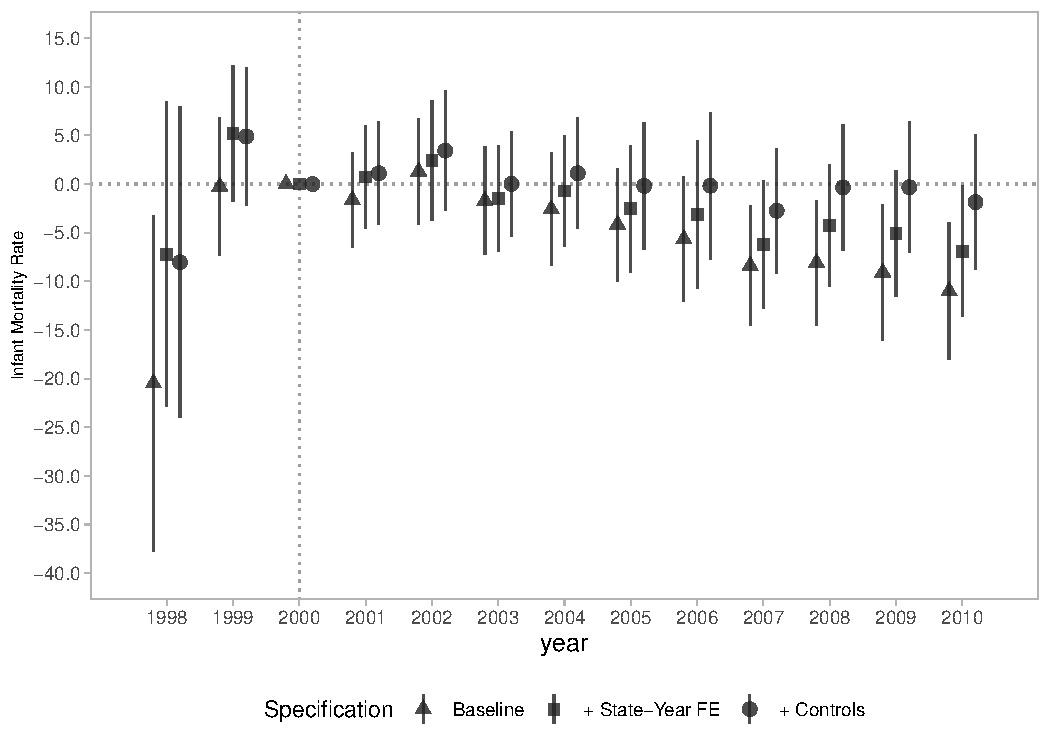
\includegraphics[width=\textwidth]{plots/IMR/tx_mi_dist_ec29_baseline_dist_ec29_baseline_full.pdf}
    \end{subfigure}
    \begin{subfigure}{0.32\textwidth}
        \centering
        \caption{\scriptsize Amenable to Primary Care}\label{fig:imr1_b}
        \includegraphics[width=\textwidth]{plots/IMR/tx_mi_icsap_dist_ec29_baseline_dist_ec29_baseline_full.pdf}
    \end{subfigure}
    \begin{subfigure}{0.32\textwidth}
        \centering
        \caption{\scriptsize Non-Amenable to Primary Care}\label{fig:imr1_c}
        \includegraphics[width=\textwidth]{plots/IMR/tx_mi_nicsap_dist_ec29_baseline_dist_ec29_baseline_full.pdf}
    \end{subfigure}
    
    \end{center}
    
\end{figure}

\begin{figure}[h]
    \begin{center}
    \caption{Causal Effects on Infant Mortality Rates - By Timing}\label{fig:imr2}
    \begin{subfigure}{0.48\textwidth}
        \caption{\scriptsize Fetal}\label{fig:imr2_a}
        \centering
        \includegraphics[width=\textwidth]{plots/IMR/tx_mi_fet_dist_ec29_baseline_dist_ec29_baseline_full.pdf}
    \end{subfigure}
    \begin{subfigure}{0.48\textwidth}
        \centering
        \caption{\scriptsize Within 24h}\label{fig:imr2_b}
        \includegraphics[width=\textwidth]{plots/IMR/tx_mi_24h_dist_ec29_baseline_dist_ec29_baseline_full.pdf}
    \end{subfigure}
    \begin{subfigure}{0.48\textwidth}
        \centering
        \caption{\scriptsize 1 to 27 days}\label{fig:imr2_c}
        \includegraphics[width=\textwidth]{plots/IMR/tx_mi_27d_dist_ec29_baseline_dist_ec29_baseline_full.pdf}
    \end{subfigure}
    \begin{subfigure}{0.48\textwidth}
        \centering
        \caption{\scriptsize 27 days to 1 year}\label{fig:imr2_d}
        \includegraphics[width=\textwidth]{plots/IMR/tx_mi_ano_dist_ec29_baseline_dist_ec29_baseline_full.pdf}
    \end{subfigure}
    
    \end{center}
    
\end{figure}


\begin{figure}[h]
    \begin{center}
    \caption{Causal Effects on Infant Mortality Rates - By Cause}\label{fig:imr3}
    \begin{subfigure}{0.32\textwidth}
        \caption{\scriptsize Infectious}\label{fig:imr3_a}
        \centering
        \includegraphics[width=\textwidth]{plots/IMR/tx_mi_infec_dist_ec29_baseline_dist_ec29_baseline_full.pdf}
    \end{subfigure}
    \begin{subfigure}{0.32\textwidth}
        \centering
        \caption{\scriptsize Respiratory}\label{fig:imr3_b}
        \includegraphics[width=\textwidth]{plots/IMR/tx_mi_resp_dist_ec29_baseline_dist_ec29_baseline_full.pdf}
    \end{subfigure}
    \begin{subfigure}{0.32\textwidth}
        \centering
        \caption{\scriptsize Perinatal}\label{fig:imr3_c}
        \includegraphics[width=\textwidth]{plots/IMR/tx_mi_perinat_dist_ec29_baseline_dist_ec29_baseline_full.pdf}
    \end{subfigure}
        \begin{subfigure}{0.32\textwidth}
        \centering
        \caption{\scriptsize Congenital}\label{fig:imr3_d}
        \includegraphics[width=\textwidth]{plots/IMR/tx_mi_cong_dist_ec29_baseline_dist_ec29_baseline_full.pdf}
    \end{subfigure}
        \begin{subfigure}{0.32\textwidth}
        \centering
        \caption{\scriptsize External}\label{fig:imr3_e}
        \includegraphics[width=\textwidth]{plots/IMR/tx_mi_ext_dist_ec29_baseline_dist_ec29_baseline_full.pdf}
    \end{subfigure}
        \begin{subfigure}{0.32\textwidth}
        \centering
        \caption{\scriptsize Nutritional}\label{fig:imr3_f}
        \includegraphics[width=\textwidth]{plots/IMR/tx_mi_nut_dist_ec29_baseline_dist_ec29_baseline_full.pdf}
    \end{subfigure}
        \begin{subfigure}{0.32\textwidth}
        \centering
        \caption{\scriptsize Other}\label{fig:imr3_g}
        \includegraphics[width=\textwidth]{plots/IMR/tx_mi_out_dist_ec29_baseline_dist_ec29_baseline_full.pdf}
    \end{subfigure}
        \begin{subfigure}{0.32\textwidth}
        \centering
        \caption{\scriptsize Ill-defined}\label{fig:imr3_h}
        \includegraphics[width=\textwidth]{plots/IMR/tx_mi_illdef_dist_ec29_baseline_dist_ec29_baseline_full.pdf}
    \end{subfigure}
    \end{center}
    
\end{figure}


\begin{figure}[h]
    \begin{center}
    \caption{Causal Effects on Birth Outcomes}\label{fig:birth}
    \begin{subfigure}{0.48\textwidth}
        \caption{\scriptsize Apgar 1}\label{fig:birth_a}
        \centering
        \includegraphics[width=\textwidth]{plots/birth/birth_apgar1_dist_ec29_baseline_dist_ec29_baseline_full.pdf}
    \end{subfigure}
    \begin{subfigure}{0.48\textwidth}
        \centering
        \caption{\scriptsize Apgar 5}\label{fig:birth_b}
        \includegraphics[width=\textwidth]{plots/birth/birth_apgar5_dist_ec29_baseline_dist_ec29_baseline_full.pdf}
    \end{subfigure}
    \begin{subfigure}{0.48\textwidth}
        \centering
        \caption{\scriptsize Low Birth Weight (<2.5k)}\label{fig:birth_c}
        \includegraphics[width=\textwidth]{plots/birth/birth_low_weight_2500g_dist_ec29_baseline_dist_ec29_baseline_full.pdf}
    \end{subfigure}
    \begin{subfigure}{0.48\textwidth}
        \centering
        \caption{\scriptsize Gestation Weeks 37+ }\label{fig:birth_d}
        \includegraphics[width=\textwidth]{plots/birth/birth_gest_37plus_dist_ec29_baseline_dist_ec29_baseline_full.pdf}
    \end{subfigure}
    
    \end{center}
    
\end{figure}



\subsection{Mechanisms: Causal Effects on Health Inputs}

\begin{table}[H]
\begin{footnotesize}
\begin{center}
\scalebox{1}{
\begin{threeparttable}[b]

  \centering
  \caption{Causal Effects on Public Health Infrastructure}
    \begin{tabular}{rrrrrr}
          &       &       &       &       &  \\
    \midrule
    \midrule
          &       & \multicolumn{4}{c}{Distance to EC9 target} \\
\cmidrule{3-6}          &       & \multicolumn{1}{c}{(1)} & \multicolumn{1}{c}{(2)} & \multicolumn{1}{c}{(3)} & \multicolumn{1}{c}{obs} \\
    \midrule
    \multicolumn{1}{p{22.715em}}{\textbf{Number of Health Facilities (per capita * 1000) with}} &       &       &       &       &  \\
    \multicolumn{1}{l}{\multirow{2}[0]{*}{Ambulatory Service}} &       & \multicolumn{1}{l}{-0.05} & \multicolumn{1}{l}{-0.09} & \multicolumn{1}{l}{-0.045} & \multicolumn{1}{c}{        49,066 } \\
          &       & \multicolumn{1}{l}{(0.068)} & \multicolumn{1}{l}{(0.055)} & \multicolumn{1}{l}{(0.044)} &  \\
    \multicolumn{1}{l}{\multirow{2}[0]{*}{Low \& Mid Complexity Ambulatory Service}} &       & \multicolumn{1}{l}{-0.056} & \multicolumn{1}{l}{-0.091*} & \multicolumn{1}{l}{-0.051} & \multicolumn{1}{c}{        49,066 } \\
          &       & \multicolumn{1}{l}{(0.067)} & \multicolumn{1}{l}{(0.055)} & \multicolumn{1}{l}{(0.044)} &  \\
    \multicolumn{1}{l}{\multirow{2}[0]{*}{High Complexity Ambulatory Service}} &       & \multicolumn{1}{l}{-0.041} & \multicolumn{1}{l}{-0.054***} & \multicolumn{1}{l}{0.007} & \multicolumn{1}{c}{        49,066 } \\
          &       & \multicolumn{1}{l}{(0.027)} & \multicolumn{1}{l}{(0.02)} & \multicolumn{1}{l}{(0.013)} &  \\
    \multicolumn{1}{l}{\multirow{2}[0]{*}{Ambulatory Service by Low Skilled Workers}} &       & \multicolumn{1}{l}{0.035} & \multicolumn{1}{l}{-0.126**} & \multicolumn{1}{l}{-0.02} & \multicolumn{1}{c}{        49,066 } \\
          &       & \multicolumn{1}{l}{(0.069)} & \multicolumn{1}{l}{(0.055)} & \multicolumn{1}{l}{(0.03)} &  \\
    \multicolumn{1}{l}{\multirow{2}[0]{*}{Ambulatory Service by Mid Skilled Workers}} &       & \multicolumn{1}{l}{0.029} & \multicolumn{1}{l}{-0.009} & \multicolumn{1}{l}{-0.025} & \multicolumn{1}{c}{        49,066 } \\
          &       & \multicolumn{1}{l}{(0.033)} & \multicolumn{1}{l}{(0.039)} & \multicolumn{1}{l}{(0.032)} &  \\
    \multicolumn{1}{l}{\multirow{2}[0]{*}{Ambulatory Service by Nurses}} &       & \multicolumn{1}{l}{0.055} & \multicolumn{1}{l}{-0.038} & \multicolumn{1}{l}{0.021} & \multicolumn{1}{c}{        49,066 } \\
          &       & \multicolumn{1}{l}{(0.046)} & \multicolumn{1}{l}{(0.037)} & \multicolumn{1}{l}{(0.026)} &  \\
    \multicolumn{1}{l}{\multirow{2}[0]{*}{Ambulatory Service by Obstetrical Nurses}} &       & \multicolumn{1}{l}{-0.002} & \multicolumn{1}{l}{-0.001} & \multicolumn{1}{l}{-0.001} & \multicolumn{1}{c}{        49,066 } \\
          &       & \multicolumn{1}{l}{(0.001)} & \multicolumn{1}{l}{(0.001)} & \multicolumn{1}{l}{(0.002)} &  \\
    \multicolumn{1}{l}{\multirow{2}[0]{*}{Ambulatory Service and Community Doctors}} &       & \multicolumn{1}{l}{0.045} & \multicolumn{1}{l}{-0.096**} & \multicolumn{1}{l}{-0.027} & \multicolumn{1}{c}{        49,066 } \\
          &       & \multicolumn{1}{l}{(0.05)} & \multicolumn{1}{l}{(0.038)} & \multicolumn{1}{l}{(0.024)} &  \\
    \multicolumn{1}{l}{\multirow{2}[0]{*}{Obstetrical/Gyneco. Ambulatory Service}} &       & \multicolumn{1}{l}{-0.022} & \multicolumn{1}{l}{0.025} & \multicolumn{1}{l}{0.012} & \multicolumn{1}{c}{        49,066 } \\
          &       & \multicolumn{1}{l}{(0.017)} & \multicolumn{1}{l}{(0.02)} & \multicolumn{1}{l}{(0.015)} &  \\
    \multicolumn{1}{l}{\multirow{2}[0]{*}{Pediatric Ambulatory Service}} &       & \multicolumn{1}{l}{-0.025} & \multicolumn{1}{l}{0.029} & \multicolumn{1}{l}{0.012} & \multicolumn{1}{c}{        49,066 } \\
          &       & \multicolumn{1}{l}{(0.018)} & \multicolumn{1}{l}{(0.022)} & \multicolumn{1}{l}{(0.016)} &  \\
    \multicolumn{1}{l}{\multirow{2}[0]{*}{Ambulatory Service and PSF Doctors}} &       & \multicolumn{1}{l}{0.05} & \multicolumn{1}{l}{-0.104***} & \multicolumn{1}{l}{-0.031} & \multicolumn{1}{c}{        49,066 } \\
          &       & \multicolumn{1}{l}{(0.05)} & \multicolumn{1}{l}{(0.039)} & \multicolumn{1}{l}{(0.025)} &  \\
    \multicolumn{1}{l}{\multirow{2}[0]{*}{Ambulatory Service and PSF Nurses}} &       & \multicolumn{1}{l}{0.057} & \multicolumn{1}{l}{-0.105***} & \multicolumn{1}{l}{-0.032} & \multicolumn{1}{c}{        49,066 } \\
          &       & \multicolumn{1}{l}{(0.051)} & \multicolumn{1}{l}{(0.039)} & \multicolumn{1}{l}{(0.025)} &  \\
    \multicolumn{1}{l}{\multirow{2}[0]{*}{Ambulatory Service and PSF Nursing Assistants}} &       & \multicolumn{1}{l}{0.055} & \multicolumn{1}{l}{-0.109***} & \multicolumn{1}{l}{-0.032} & \multicolumn{1}{c}{        49,066 } \\
          &       & \multicolumn{1}{l}{(0.049)} & \multicolumn{1}{l}{(0.038)} & \multicolumn{1}{l}{(0.024)} &  \\
    \multicolumn{1}{l}{\multirow{2}[0]{*}{Ambulatory Service and PSF Teams}} &       & \multicolumn{1}{l}{0.05} & \multicolumn{1}{l}{-0.115***} & \multicolumn{1}{l}{-0.038} & \multicolumn{1}{c}{        49,066 } \\
          &       & \multicolumn{1}{l}{(0.053)} & \multicolumn{1}{l}{(0.042)} & \multicolumn{1}{l}{(0.026)} &  \\
    \multicolumn{1}{l}{\multirow{2}[0]{*}{Ambulatory Service and ACS Teams}} &       & \multicolumn{1}{l}{0.021} & \multicolumn{1}{l}{-0.087**} & \multicolumn{1}{l}{-0.036} & \multicolumn{1}{c}{        49,066 } \\
          &       & \multicolumn{1}{l}{(0.041)} & \multicolumn{1}{l}{(0.034)} & \multicolumn{1}{l}{(0.027)} &  \\
    \multicolumn{1}{l}{\multirow{2}[0]{*}{Ambulatory Service and ACS Nurses}} &       & \multicolumn{1}{l}{-0.025**} & \multicolumn{1}{l}{0.011} & \multicolumn{1}{l}{0.001} & \multicolumn{1}{c}{        49,066 } \\
          &       & \multicolumn{1}{l}{(0.012)} & \multicolumn{1}{l}{(0.011)} & \multicolumn{1}{l}{(0.011)} &  \\
          &       &       &       &       &  \\
    \midrule
    \midrule
          &       &       &       &       &  \\
    \end{tabular}%
    
  \label{table:infra}%

\end{threeparttable}
}
\end{center}
\end{footnotesize}
\end{table}

\begin{table}[H]
\begin{footnotesize}
\begin{center}
\scalebox{0.9}{
\begin{threeparttable}[b]

  \centering
  \caption{Causal Effects on Access to Healthcare}
    \begin{tabular}{rrrrrr}
          &       &       &       &       &  \\
    \midrule
    \midrule
          &       & \multicolumn{4}{c}{Distance to EC9 target} \\
\cmidrule{3-6}          &       & \multicolumn{1}{c}{(1)} & \multicolumn{1}{c}{(2)} & \multicolumn{1}{c}{(3)} & \multicolumn{1}{c}{obs} \\
    \midrule
    \multicolumn{1}{p{19.07em}}{\textbf{Primary Care Coverage -  Extensive Margin}} &       &       &       &       &  \\
    \multicolumn{1}{l}{\multirow{2}[0]{*}{Population covered (share) by Community Health Agents}} &       & \multicolumn{1}{c}{-0.064} & \multicolumn{1}{c}{0.168} & \multicolumn{1}{c}{0.189*} & \multicolumn{1}{c}{   64,327 } \\
          &       & \multicolumn{1}{c}{(0.119)} & \multicolumn{1}{c}{(0.12)} & \multicolumn{1}{c}{(0.11)} &  \\
    \multicolumn{1}{l}{\multirow{2}[0]{*}{Population covered (share) by Family Health Agents}} &       & \multicolumn{1}{c}{0.187} & \multicolumn{1}{c}{-0.111} & \multicolumn{1}{c}{0.006} & \multicolumn{1}{c}{   64,327 } \\
          &       & \multicolumn{1}{c}{(0.165)} & \multicolumn{1}{c}{(0.143)} & \multicolumn{1}{c}{(0.116)} &  \\
    \multicolumn{1}{l}{\multirow{2}[0]{*}{N. of People Register in the Primary Care System (per capita)}} &       & \multicolumn{1}{c}{-0.02} & \multicolumn{1}{c}{-0.042} & \multicolumn{1}{c}{0.005} & \multicolumn{1}{c}{   64,327 } \\
          &       & \multicolumn{1}{c}{(0.163)} & \multicolumn{1}{c}{(0.146)} & \multicolumn{1}{c}{(0.132)} &  \\
    \multicolumn{1}{l}{\multirow{2}[0]{*}{N. of People Register in the CH Program (per capita)}} &       & \multicolumn{1}{c}{-0.254**} & \multicolumn{1}{c}{0.073} & \multicolumn{1}{c}{-0.041} & \multicolumn{1}{c}{   64,327 } \\
          &       & \multicolumn{1}{c}{(0.11)} & \multicolumn{1}{c}{(0.107)} & \multicolumn{1}{c}{(0.099)} &  \\
    \multicolumn{1}{l}{\multirow{2}[0]{*}{N. of People Register in the FH Program (per capita)}} &       & \multicolumn{1}{c}{0.234} & \multicolumn{1}{c}{-0.113} & \multicolumn{1}{c}{0.048} & \multicolumn{1}{c}{   64,327 } \\
          &       & \multicolumn{1}{c}{(0.168)} & \multicolumn{1}{c}{(0.126)} & \multicolumn{1}{c}{(0.095)} &  \\
    \multicolumn{1}{p{19.07em}}{\textbf{Primary Care Coverage -  Intensive Margin}} &       &       &       &       &  \\
    \multicolumn{1}{l}{\multirow{2}[0]{*}{N. of People Visited by Primary Care Agents (per capita)}} &       & \multicolumn{1}{c}{-0.101} & \multicolumn{1}{c}{-0.145} & \multicolumn{1}{c}{0.083} & \multicolumn{1}{c}{   64,327 } \\
          &       & \multicolumn{1}{c}{(0.196)} & \multicolumn{1}{c}{(0.164)} & \multicolumn{1}{c}{(0.12)} &  \\
    \multicolumn{1}{l}{\multirow{2}[0]{*}{N. of People Visited by Community Health Agents (per capita)}} &       & \multicolumn{1}{c}{-0.117*} & \multicolumn{1}{c}{-0.033} & \multicolumn{1}{c}{-0.074} & \multicolumn{1}{c}{   64,327 } \\
          &       & \multicolumn{1}{c}{(0.069)} & \multicolumn{1}{c}{(0.069)} & \multicolumn{1}{c}{(0.062)} &  \\
    \multicolumn{1}{l}{\multirow{2}[0]{*}{N. of People Visited by Family Health Agents (per capita)}} &       & \multicolumn{1}{c}{0.017} & \multicolumn{1}{c}{-0.11} & \multicolumn{1}{c}{0.16} & \multicolumn{1}{c}{   64,327 } \\
          &       & \multicolumn{1}{c}{(0.213)} & \multicolumn{1}{c}{(0.187)} & \multicolumn{1}{c}{(0.131)} &  \\
    \multicolumn{1}{l}{\multirow{2}[0]{*}{N. of Household Visits (per capita)}} &       & \multicolumn{1}{c}{-0.165} & \multicolumn{1}{c}{0.205} & \multicolumn{1}{c}{0.579**} & \multicolumn{1}{c}{   64,327 } \\
          &       & \multicolumn{1}{c}{(0.422)} & \multicolumn{1}{c}{(0.357)} & \multicolumn{1}{c}{(0.293)} &  \\
    \multicolumn{1}{l}{\multirow{2}[0]{*}{N. of Household Visits by Community Health Agents (per capita)}} &       & \multicolumn{1}{c}{-0.89***} & \multicolumn{1}{c}{0.619***} & \multicolumn{1}{c}{0.312*} & \multicolumn{1}{c}{   64,327 } \\
          &       & \multicolumn{1}{c}{(0.269)} & \multicolumn{1}{c}{(0.238)} & \multicolumn{1}{c}{(0.187)} &  \\
    \multicolumn{1}{l}{\multirow{2}[0]{*}{N. of Household Visits by Family Health Agents (per capita)}} &       & \multicolumn{1}{c}{0.716} & \multicolumn{1}{c}{-0.413} & \multicolumn{1}{c}{0.276} & \multicolumn{1}{c}{   64,327 } \\
          &       & \multicolumn{1}{c}{(0.549)} & \multicolumn{1}{c}{(0.436)} & \multicolumn{1}{c}{(0.296)} &  \\
    \multicolumn{1}{l}{\multirow{2}[0]{*}{N. of Appointments (per capita)}} &       & \multicolumn{1}{c}{0.08} & \multicolumn{1}{c}{-0.134} & \multicolumn{1}{c}{0.035} & \multicolumn{1}{c}{   64,327 } \\
          &       & \multicolumn{1}{c}{(0.112)} & \multicolumn{1}{c}{(0.098)} & \multicolumn{1}{c}{(0.083)} &  \\
    \multicolumn{1}{l}{\multirow{2}[0]{*}{N. of Appointments from Community Health Program (per capita)}} &       & \multicolumn{1}{c}{0.052*} & \multicolumn{1}{c}{0.023} & \multicolumn{1}{c}{0.018} & \multicolumn{1}{c}{   64,327 } \\
          &       & \multicolumn{1}{c}{(0.028)} & \multicolumn{1}{c}{(0.025)} & \multicolumn{1}{c}{(0.022)} &  \\
    \multicolumn{1}{l}{\multirow{2}[0]{*}{N. of Appointments from Family Health Program (per capita)}} &       & \multicolumn{1}{c}{0.08} & \multicolumn{1}{c}{-0.134} & \multicolumn{1}{c}{0.035} & \multicolumn{1}{c}{   64,327 } \\
          &       & \multicolumn{1}{c}{(0.112)} & \multicolumn{1}{c}{(0.098)} & \multicolumn{1}{c}{(0.083)} &  \\
    \multicolumn{1}{p{19.07em}}{\textbf{Access to Health Services}} &       &       &       &       &  \\
    \multicolumn{1}{l}{\multirow{2}[0]{*}{Share of C-Section}} &       & \multicolumn{1}{c}{0.063**} & \multicolumn{1}{c}{-0.024} & \multicolumn{1}{c}{-0.017} & \multicolumn{1}{c}{   64,327 } \\
          &       & \multicolumn{1}{c}{(0.029)} & \multicolumn{1}{c}{(0.021)} & \multicolumn{1}{c}{(0.018)} &  \\
    \multicolumn{1}{l}{\multirow{2}[0]{*}{Prenatal Visits None}} &       & \multicolumn{1}{c}{-0.086***} & \multicolumn{1}{c}{0.019} & \multicolumn{1}{c}{0.002} & \multicolumn{1}{c}{   64,327 } \\
          &       & \multicolumn{1}{c}{(0.018)} & \multicolumn{1}{c}{(0.013)} & \multicolumn{1}{c}{(0.01)} &  \\
    \multicolumn{1}{l}{\multirow{2}[0]{*}{Prenatal Visits 1-6}} &       & \multicolumn{1}{c}{0.388***} & \multicolumn{1}{c}{0.132**} & \multicolumn{1}{c}{0.122**} & \multicolumn{1}{c}{   64,327 } \\
          &       & \multicolumn{1}{c}{(0.091)} & \multicolumn{1}{c}{(0.058)} & \multicolumn{1}{c}{(0.06)} &  \\
    \multicolumn{1}{l}{\multirow{2}[0]{*}{Prenatal Visits 7+}} &       & \multicolumn{1}{c}{-0.281***} & \multicolumn{1}{c}{-0.046} & \multicolumn{1}{c}{-0.03} & \multicolumn{1}{c}{   64,327 } \\
          &       & \multicolumn{1}{c}{(0.099)} & \multicolumn{1}{c}{(0.075)} & \multicolumn{1}{c}{(0.062)} &  \\
          &       &       &       &       &  \\
    \midrule
    \midrule
          &       &       &       &       &  \\
    \end{tabular}%
    
  \label{table:access}%

\end{threeparttable}
}
\end{center}
\end{footnotesize}
\end{table}

\begin{table}[H]
\begin{footnotesize}
\begin{center}
\scalebox{0.9}{
\begin{threeparttable}[b]

  \centering
  \caption{Causal Effects on Ambulatorial Production}
    \begin{tabular}{rrrrrr}
          &       &       &       &       &  \\
    \midrule
    \midrule
          &       & \multicolumn{4}{c}{Distance to EC9 target} \\
\cmidrule{3-6}          &       & \multicolumn{1}{c}{(1)} & \multicolumn{1}{c}{(2)} & \multicolumn{1}{c}{(3)} & \multicolumn{1}{c}{obs} \\
    \midrule
    \multicolumn{1}{p{26.355em}}{\textbf{Ambulatorial Production}} &       &       &       &       &  \\
    \multicolumn{1}{l}{\multirow{2}[0]{*}{Outpatient procedures per capita}} &       & \multicolumn{1}{l}{0.49} & \multicolumn{1}{l}{5.135*} & \multicolumn{1}{l}{0.54} & \multicolumn{1}{c}{     64,327 } \\
          &       & \multicolumn{1}{l}{(2.754)} & \multicolumn{1}{l}{(2.685)} & \multicolumn{1}{l}{(2.023)} &  \\
    \multicolumn{1}{l}{\multirow{2}[0]{*}{Primary Care Outpatient procedures per capita}} &       & \multicolumn{1}{l}{1.3} & \multicolumn{1}{l}{0.552} & \multicolumn{1}{l}{2.54**} & \multicolumn{1}{c}{     64,327 } \\
          &       & \multicolumn{1}{l}{(1.729)} & \multicolumn{1}{l}{(1.53)} & \multicolumn{1}{l}{(1.262)} &  \\
    \multicolumn{1}{l}{\multirow{2}[0]{*}{N. of Low \& Mid Complexity Outpatient Procedures (per capita)}} &       & \multicolumn{1}{l}{2.59} & \multicolumn{1}{l}{2.297} & \multicolumn{1}{l}{4.046*} & \multicolumn{1}{c}{     49,066 } \\
          &       & \multicolumn{1}{l}{(2.276)} & \multicolumn{1}{l}{(2.912)} & \multicolumn{1}{l}{(2.239)} &  \\
    \multicolumn{1}{l}{\multirow{2}[0]{*}{N. of High Complexity Outpatient Procedures (per capita)}} &       & \multicolumn{1}{l}{-0.887**} & \multicolumn{1}{l}{-0.729***} & \multicolumn{1}{l}{-0.126} & \multicolumn{1}{c}{     49,066 } \\
          &       & \multicolumn{1}{l}{(0.391)} & \multicolumn{1}{l}{(0.267)} & \multicolumn{1}{l}{(0.179)} &  \\
    \multicolumn{1}{l}{\multirow{2}[0]{*}{N. of Outpatient Procedures by Low Skilled Workers (per capita)}} &       & \multicolumn{1}{l}{-1.278**} & \multicolumn{1}{l}{-0.942} & \multicolumn{1}{l}{0.035} & \multicolumn{1}{c}{     49,066 } \\
          &       & \multicolumn{1}{l}{(0.563)} & \multicolumn{1}{l}{(0.585)} & \multicolumn{1}{l}{(0.465)} &  \\
    \multicolumn{1}{l}{\multirow{2}[0]{*}{N. of Outpatient procedures by Mid Skilled Workers (per capita)}} &       & \multicolumn{1}{l}{0.573} & \multicolumn{1}{l}{0.47} & \multicolumn{1}{l}{-0.187} & \multicolumn{1}{c}{     49,066 } \\
          &       & \multicolumn{1}{l}{(0.761)} & \multicolumn{1}{l}{(1.107)} & \multicolumn{1}{l}{(0.842)} &  \\
          &       &       &       &       &  \\
    \midrule
    \midrule
          &       &       &       &       &  \\
    \end{tabular}%
    
  \label{table:ambulatorial}%

\end{threeparttable}
}
\end{center}
\end{footnotesize}
\end{table}



\begin{figure}[h]
    \begin{center}
    \caption{Causal Effects on the Number of Health Facilities (per capita*1000) with:}\label{fig:infra}
    \begin{subfigure}{0.24\textwidth}
        \caption{\tiny Ambulatory Service}\label{fig:infra_a}
        \centering
        \includegraphics[width=\textwidth]{plots/infra/sia_ncnes_amb_mun_pcapita_dist_ec29_baseline_dist_ec29_baseline_full.pdf}
    \end{subfigure}
    \begin{subfigure}{0.24\textwidth}
        \centering
        \caption{\tiny Low & Mid Complexity Ambulatory Service}\label{fig:infra_b}
        \includegraphics[width=\textwidth]{plots/infra/sia_ncnes_amb_lc_mun_pcapita_dist_ec29_baseline_dist_ec29_baseline_full.pdf}
    \end{subfigure}
    \begin{subfigure}{0.24\textwidth}
        \centering
        \caption{\tiny High Complexity Ambulatory Service}\label{fig:infra_c}
        \includegraphics[width=\textwidth]{plots/infra/sia_ncnes_amb_hc_mun_pcapita_dist_ec29_baseline_dist_ec29_baseline_full.pdf}
    \end{subfigure}
    \begin{subfigure}{0.24\textwidth}
        \centering
        \caption{\tiny Ambulatory Service by Low Skilled Workers}\label{fig:infra_d}
        \includegraphics[width=\textwidth]{plots/infra/sia_ncnes_low_skill_mun_pcapita_dist_ec29_baseline_dist_ec29_baseline_full.pdf}
    \end{subfigure}
    \begin{subfigure}{0.24\textwidth}
        \centering
        \caption{\tiny Ambulatory Service by Mid Skilled Workers}\label{fig:infra_e}
        \includegraphics[width=\textwidth]{plots/infra/sia_ncnes_med_skill_mun_pcapita_dist_ec29_baseline_dist_ec29_baseline_full.pdf}
    \end{subfigure}
    \begin{subfigure}{0.24\textwidth}
        \centering
        \caption{\tiny Ambulatory Service by Nurses}\label{fig:infra_f}
        \includegraphics[width=\textwidth]{plots/infra/sia_ncnes_enf_mun_pcapita_dist_ec29_baseline_dist_ec29_baseline_full.pdf}
    \end{subfigure}
    \begin{subfigure}{0.24\textwidth}
        \centering
        \caption{\tiny Ambulatory Service by Obstetrical Nurses}\label{fig:infra_g}
        \includegraphics[width=\textwidth]{plots/infra/sia_ncnes_enfobs_mun_pcapita_dist_ec29_baseline_dist_ec29_baseline_full.pdf}
    \end{subfigure}
    \begin{subfigure}{0.24\textwidth}
        \centering
        \caption{\tiny Ambulatory Service and Community Doctors}\label{fig:infra_h}
        \includegraphics[width=\textwidth]{plots/infra/sia_ncnes_medcom_pcapita_dist_ec29_baseline_dist_ec29_baseline_full.pdf}
    \end{subfigure}
    \begin{subfigure}{0.24\textwidth}
        \centering
        \caption{\tiny Obstetrical/Gyneco. Ambulatory Service}\label{fig:infra_i}
        \includegraphics[width=\textwidth]{plots/infra/sia_ncnes_ginobs_mun_pcapita_dist_ec29_baseline_dist_ec29_baseline_full.pdf}
    \end{subfigure}
    \begin{subfigure}{0.24\textwidth}
        \centering
        \caption{\tiny Pediatric Ambulatory Service}\label{fig:infra_j}
        \includegraphics[width=\textwidth]{plots/infra/sia_ncnes_pediat_mun_pcapita_dist_ec29_baseline_dist_ec29_baseline_full.pdf}
    \end{subfigure}
    \begin{subfigure}{0.24\textwidth}
        \centering
        \caption{\tiny Ambulatory Service and PSF Doctors}\label{fig:infra_k}
        \includegraphics[width=\textwidth]{plots/infra/sia_ncnes_medpsf_pcapita_dist_ec29_baseline_dist_ec29_baseline_full.pdf}
    \end{subfigure}
    \begin{subfigure}{0.24\textwidth}
        \centering
        \caption{\tiny Ambulatory Service and PSF Nurses}\label{fig:infra_l}
        \includegraphics[width=\textwidth]{plots/infra/sia_ncnes_enfpsf_pcapita_dist_ec29_baseline_dist_ec29_baseline_full.pdf}
    \end{subfigure}
    \begin{subfigure}{0.24\textwidth}
        \centering
        \caption{\tiny Ambulatory Service and PSF Nursing Assistants}\label{fig:infra_m}
        \includegraphics[width=\textwidth]{plots/infra/sia_ncnes_outpsf_pcapita_dist_ec29_baseline_dist_ec29_baseline_full.pdf}
    \end{subfigure}
    \begin{subfigure}{0.24\textwidth}
        \centering
        \caption{\tiny Ambulatory Service and PSF Teams}\label{fig:infra_n}
        \includegraphics[width=\textwidth]{plots/infra/sia_ncnes_psf_pcapita_dist_ec29_baseline_dist_ec29_baseline_full.pdf}
    \end{subfigure}
    \begin{subfigure}{0.24\textwidth}
        \centering
        \caption{\tiny Ambulatory Service and ACS Teams}\label{fig:infra_o}
        \includegraphics[width=\textwidth]{plots/infra/sia_ncnes_acs_pcapita_dist_ec29_baseline_dist_ec29_baseline_full.pdf}
    \end{subfigure}
    \begin{subfigure}{0.24\textwidth}
        \centering
        \caption{\tiny Ambulatory Service and ACS Nurses}\label{fig:infra_p}
        \includegraphics[width=\textwidth]{plots/infra/sia_ncnes_enfacs_pcapita_dist_ec29_baseline_dist_ec29_baseline_full.pdf}
    \end{subfigure}
    
    \end{center}
    
\end{figure}


\begin{figure}[h]
    \begin{center}
    \caption{Causal Effects on Primary Care Coverage - Extensive Margin}\label{fig:access1}
    \begin{subfigure}{0.32\textwidth}
        \caption{\scriptsize Population covered (share) by Community Health Agents}\label{fig:access1_a}
        \centering
        \includegraphics[width=\textwidth]{plots/access/ACS_popprop_dist_ec29_baseline_dist_ec29_baseline_full.pdf}
    \end{subfigure}
    \begin{subfigure}{0.32\textwidth}
        \centering
        \caption{\scriptsize Population covered (share) by Family Health Agents}\label{fig:iaccess1_b}
        \includegraphics[width=\textwidth]{plots/access/eSF_popprop_dist_ec29_baseline_dist_ec29_baseline_full.pdf}
    \end{subfigure}
    \begin{subfigure}{0.32\textwidth}
        \centering
        \caption{\scriptsize N. of People Register in the Primary Care System (per capita)}\label{fig:access1_c}
        \includegraphics[width=\textwidth]{plots/access/siab_regist_pers_pcapita_dist_ec29_baseline_dist_ec29_baseline_full.pdf}
    \end{subfigure}
    \begin{subfigure}{0.32\textwidth}
        \centering
        \caption{\scriptsize N. of People Register in the CH Program (per capita)}\label{fig:access1_d}
        \includegraphics[width=\textwidth]{plots/access/siab_regist_pers_pacs_pcapita_dist_ec29_baseline_dist_ec29_baseline_full.pdf}
    \end{subfigure}
    \begin{subfigure}{0.32\textwidth}
        \centering
        \caption{\scriptsize N. of People Register in the FH Program (per capita)}\label{fig:access1_e}
        \includegraphics[width=\textwidth]{plots/access/siab_regist_pers_psf_pcapita_dist_ec29_baseline_dist_ec29_baseline_full.pdf}
    \end{subfigure}
    
    
    \end{center}
    
\end{figure}

\begin{figure}[h]
    \begin{center}
    \caption{Causal Effects on Primary Care Coverage - Intensive Margin}\label{fig:access2}
    \begin{subfigure}{0.32\textwidth}
        \caption{\scriptsize N. of People Visited by Primary Care Agents (per capita)}\label{fig:access2_a}
        \centering
        \includegraphics[width=\textwidth]{plots/access/siab_accomp_especif_pcapita_dist_ec29_baseline_dist_ec29_baseline_full.pdf}
    \end{subfigure}
    \begin{subfigure}{0.32\textwidth}
        \centering
        \caption{\scriptsize N. of People Visited by Community Health Agents (per capita)}\label{fig:iaccess2_b}
        \includegraphics[width=\textwidth]{plots/access/siab_accomp_especif_pacs_pcapita_dist_ec29_baseline_dist_ec29_baseline_full.pdf}
    \end{subfigure}
    \begin{subfigure}{0.32\textwidth}
        \centering
        \caption{\scriptsize N. of People Visited by Family Health Agents (per capita)}\label{fig:access2_c}
        \includegraphics[width=\textwidth]{plots/access/siab_accomp_especif_psf_pcapita_dist_ec29_baseline_dist_ec29_baseline_full.pdf}
    \end{subfigure}
    \begin{subfigure}{0.32\textwidth}
        \centering
        \caption{\scriptsize N. of Household Visits (per capita)}\label{fig:access2_d}
        \includegraphics[width=\textwidth]{plots/access/siab_visit_cha_pcapita_dist_ec29_baseline_dist_ec29_baseline_full.pdf}
    \end{subfigure}
    \begin{subfigure}{0.32\textwidth}
        \centering
        \caption{\scriptsize N. of Household Visits by Community Health Agents (per capita)}\label{fig:access2_e}
        \includegraphics[width=\textwidth]{plots/access/siab_visit_cha_pacs_pcapita_dist_ec29_baseline_dist_ec29_baseline_full.pdf}
    \end{subfigure}
    \begin{subfigure}{0.32\textwidth}
        \centering
        \caption{\scriptsize N. of Household Visits by Family Health Agents (per capita)}\label{fig:access2_f}
        \includegraphics[width=\textwidth]{plots/access/siab_visit_cha_psf_pcapita_dist_ec29_baseline_dist_ec29_baseline_full.pdf}
    \end{subfigure}
    \begin{subfigure}{0.32\textwidth}
        \centering
        \caption{\scriptsize N. of Appointments (per capita)}\label{fig:access2_g}
        \includegraphics[width=\textwidth]{plots/access/siab_cons_especif_pcapita_dist_ec29_baseline_dist_ec29_baseline_full.pdf}
    \end{subfigure}
    \begin{subfigure}{0.32\textwidth}
        \centering
        \caption{\scriptsize N. of Appointments from Community Health Program (per capita)}\label{fig:access2_h}
        \includegraphics[width=\textwidth]{plots/access/siab_cons_especif_pacs_pcapita_dist_ec29_baseline_dist_ec29_baseline_full.pdf}
    \end{subfigure}
    \begin{subfigure}{0.32\textwidth}
        \centering
        \caption{\scriptsize N. of Appointments from Family Health Program (per capita)}\label{fig:access2_i}
        \includegraphics[width=\textwidth]{plots/access/siab_accomp_especif_psf_pcapita_dist_ec29_baseline_dist_ec29_baseline_full.pdf}
    \end{subfigure}
    
    
    \end{center}
    
\end{figure}

\begin{figure}[h]
    \begin{center}
    \caption{Causal Effects on Access to Health Services}\label{fig:access3}
    \begin{subfigure}{0.48\textwidth}
        \caption{\scriptsize Share of C-Section)}\label{fig:access3_a}
        \centering
        \includegraphics[width=\textwidth]{plots/birth/birth_c_sections_dist_ec29_baseline_dist_ec29_baseline_full.pdf}
    \end{subfigure}
    \begin{subfigure}{0.48\textwidth}
        \centering
        \caption{\scriptsize Prenatal Visits None)}\label{fig:iaccess3_b}
        \includegraphics[width=\textwidth]{plots/birth/birth_prenat_0_dist_ec29_baseline_dist_ec29_baseline_full.pdf}
    \end{subfigure}
    \begin{subfigure}{0.48\textwidth}
        \centering
        \caption{\scriptsize Prenatal Visits 1-6)}\label{fig:access3_c}
        \includegraphics[width=\textwidth]{plots/birth/birth_prenat_1_6_dist_ec29_baseline_dist_ec29_baseline_full.pdf}
    \end{subfigure}
    \begin{subfigure}{0.48\textwidth}
        \centering
        \caption{\scriptsize Prenatal Visits 7+)}\label{fig:access3_d}
        \includegraphics[width=\textwidth]{plots/birth/birth_prenat_7_plus_dist_ec29_baseline_dist_ec29_baseline_full.pdf}
    \end{subfigure}
    
    
    
    \end{center}
    
\end{figure}


\begin{figure}[h]
    \begin{center}
    \caption{Causal Effects on Ambulatorial Production}\label{fig:amb}
    \begin{subfigure}{0.32\textwidth}
        \caption{\scriptsize Outpatient procedures per capita)}\label{fig:amb_a}
        \centering
        \includegraphics[width=\textwidth]{plots/ambulatorial/sia_pcapita_dist_ec29_baseline_dist_ec29_baseline_full.pdf}
    \end{subfigure}
    \begin{subfigure}{0.32\textwidth}
        \centering
        \caption{\scriptsize Primary Care Outpatient procedures per capita)}\label{fig:amb_b}
        \includegraphics[width=\textwidth]{plots/ambulatorial/sia_ab_pcapita_dist_ec29_baseline_dist_ec29_baseline_full.pdf}
    \end{subfigure}
    \begin{subfigure}{0.32\textwidth}
        \centering
        \caption{\scriptsize N. of Low & Mid Complexity Outpatient Procedures (per capita))}\label{fig:amb_c}
        \includegraphics[width=\textwidth]{plots/ambulatorial/sia_nprod_amb_lc_mun_pcapita_dist_ec29_baseline_dist_ec29_baseline_full.pdf}
    \end{subfigure}
    \begin{subfigure}{0.32\textwidth}
        \centering
        \caption{\scriptsize N. of High Complexity Outpatient Procedures (per capita))}\label{fig:amb_d}
        \includegraphics[width=\textwidth]{plots/ambulatorial/sia_nprod_amb_hc_mun_pcapita_dist_ec29_baseline_dist_ec29_baseline_full.pdf}
    \end{subfigure}
    \begin{subfigure}{0.32\textwidth}
        \centering
        \caption{\scriptsize N. of Outpatient Procedures by Low Skilled Workers (per capita))}\label{fig:amb_e}
        \includegraphics[width=\textwidth]{plots/ambulatorial/sia_nprod_low_skill_mun_pcapita_dist_ec29_baseline_dist_ec29_baseline_full.pdf}
    \end{subfigure}
    \begin{subfigure}{0.32\textwidth}
        \centering
        \caption{\scriptsize N. of Outpatient procedures by Mid Skilled Workers (per capita))}\label{fig:amb_f}
        \includegraphics[width=\textwidth]{plots/ambulatorial/sia_nprod_med_skill_mun_pcapita_dist_ec29_baseline_dist_ec29_baseline_full.pdf}
    \end{subfigure}
    
    
    
    
    \end{center}
    
\end{figure}
% \section{Conclusions}\label{sec:conclusion}
\setstretch{1.5}

Our empirical analysis has demonstrated that when municipalities are induced to increase public health spending they do so by increasing mainly spending relative to the administrative structure of public health - roughly half of the increase -  followed by spending with investments and human resources. We also demonstrate that this increase is associated with a higher number of administrative professionals, greater supply of municipal hospitals, and greater primary care coverage at the intensive margin, with also a higher number of health facilities with primary care related professionals. The shifts in spending and health inputs are associated with small to moderate reductions in infant mortality rates related to improvements in primary care access, and long term reductions in total infant mortality rates. \cite{bhalotra2019can} have shown that the combination of access to primary and hospital care leads to better health outcomes relative to only primary care. This is a plausible channel through which the increase in the supply of municipal hospitals might be affecting infant mortality in our analysis.

These results are extremely relevant, specially in a context of a universal an decentralized health system, where provision of health care occurs mainly at the municipal level, and the majority of the resources spent locally comes from local tax incomes, in opposition to intergovernmental transfers. [Discuss transfers vs own resource spending]. We are not able to formally test exactly how health inputs and outcomes would react if municipalities allocated less resources on administrative structure and more resources into investments and personnel, but the evidence here present indicates it could lead to further improvements in health outcomes, and, thus, a more efficient use of resources within the public health sector. 


\pagebreak
\singlespacing  
\bibliographystyle{apalike}
\bibliography{SRC}
\nocite{}




\pagebreak
\appendix
\singlespacing	

\LARGE{\textbf{Appendix}}


\counterwithin{figure}{section}
\counterwithin{table}{section}



\section{Descriptive Statistics}\label{app:stats}

\begin{table}[H]
\begin{footnotesize}
\begin{center}
\scalebox{0.8}{
\begin{threeparttable}[b]

  \centering
  \caption{Descriptive Statistics (at the baseline year)}
    
    \begin{tabular}{rrrrrrrr}
          &       &       &       &       &       &       &  \\
    \midrule
    \midrule
          & \multicolumn{1}{c}{Mean} & \multicolumn{1}{c}{Std. Dev.} & \multicolumn{1}{c}{Min} & \multicolumn{1}{c}{Max} & \multicolumn{1}{c}{Obs.} &       & \multicolumn{1}{c}{Source of Data} \\
\cmidrule{1-6}\cmidrule{8-8}    \multicolumn{1}{l}{\textbf{EC 29 Variables}} &       &       &       &       &       &       &  \\
    \multicolumn{1}{l}{Share of Municipality's Own Resource Spent in Public Health} & \multicolumn{1}{c}{0.14} & \multicolumn{1}{c}{0.07} & \multicolumn{1}{c}{0.00} & \multicolumn{1}{c}{0.80} & \multicolumn{1}{c}{5224} &       & \multicolumn{1}{c}{Datasus/SIOPS} \\
    \multicolumn{1}{l}{Distance to the EC29 Target} & \multicolumn{1}{c}{0.01} & \multicolumn{1}{c}{0.07} & \multicolumn{1}{c}{-0.65} & \multicolumn{1}{c}{0.15} & \multicolumn{1}{c}{5224} &       & \multicolumn{1}{c}{Datasus/SIOPS} \\
          &       &       &       &       &       &       &  \\
    \multicolumn{1}{l}{\textbf{Public Revenue}} &       &       &       &       &       &       &  \\
    \multicolumn{1}{l}{Total Revenue per capita} & \multicolumn{1}{c}{1225.27} & \multicolumn{1}{c}{2282.13} & \multicolumn{1}{c}{132.39} & \multicolumn{1}{c}{\#\#\#\#\#\#\#\#} & \multicolumn{1}{c}{5288} &       & \multicolumn{1}{c}{Finbra} \\
          &       &       &       &       &       &       &  \\
    \multicolumn{1}{l}{\textbf{Public Spending}} &       &       &       &       &       &       &  \\
    \multicolumn{1}{l}{Total Spending per capita} & \multicolumn{1}{c}{1284.77} & \multicolumn{1}{c}{2395.06} & \multicolumn{1}{c}{129.74} & \multicolumn{1}{c}{\#\#\#\#\#\#\#\#} & \multicolumn{1}{c}{5304} &       & \multicolumn{1}{c}{Finbra} \\
          &       &       &       &       &       &       &  \\
    \multicolumn{1}{l}{Spending by Type - per capita} &       &       &       &       &       &       &  \\
    \multicolumn{1}{l}{Human Resources} & \multicolumn{1}{c}{502.32} & \multicolumn{1}{c}{985.60} & \multicolumn{1}{c}{0.00} & \multicolumn{1}{c}{60697.09} & \multicolumn{1}{c}{5304} &       & \multicolumn{1}{c}{Finbra} \\
    \multicolumn{1}{l}{Investment} & \multicolumn{1}{c}{153.70} & \multicolumn{1}{c}{277.13} & \multicolumn{1}{c}{0.00} & \multicolumn{1}{c}{14815.46} & \multicolumn{1}{c}{5304} &       & \multicolumn{1}{c}{Finbra} \\
    \multicolumn{1}{l}{Other} & \multicolumn{1}{c}{628.75} & \multicolumn{1}{c}{1280.34} & \multicolumn{1}{c}{0.00} & \multicolumn{1}{c}{79994.44} & \multicolumn{1}{c}{5304} &       & \multicolumn{1}{c}{Finbra} \\
          &       &       &       &       &       &       &  \\
    \multicolumn{1}{l}{Spending by Category - per capita} &       &       &       &       &       &       &  \\
    \multicolumn{1}{l}{Health and Sanitation} & \multicolumn{1}{c}{217.08} & \multicolumn{1}{c}{276.14} & \multicolumn{1}{c}{0.04} & \multicolumn{1}{c}{12559.61} & \multicolumn{1}{c}{5286} &       & \multicolumn{1}{c}{Finbra} \\
    \multicolumn{1}{l}{Transport} & \multicolumn{1}{c}{91.55} & \multicolumn{1}{c}{138.28} & \multicolumn{1}{c}{0.00} & \multicolumn{1}{c}{5865.79} & \multicolumn{1}{c}{5304} &       & \multicolumn{1}{c}{Finbra} \\
    \multicolumn{1}{l}{Education and Culture} & \multicolumn{1}{c}{419.95} & \multicolumn{1}{c}{640.29} & \multicolumn{1}{c}{0.00} & \multicolumn{1}{c}{36319.15} & \multicolumn{1}{c}{5304} &       & \multicolumn{1}{c}{Finbra} \\
    \multicolumn{1}{l}{Housing and Urban} & \multicolumn{1}{c}{116.05} & \multicolumn{1}{c}{301.25} & \multicolumn{1}{c}{0.00} & \multicolumn{1}{c}{19842.15} & \multicolumn{1}{c}{5304} &       & \multicolumn{1}{c}{Finbra} \\
    \multicolumn{1}{l}{Social Assistance} & \multicolumn{1}{c}{84.05} & \multicolumn{1}{c}{253.84} & \multicolumn{1}{c}{0.00} & \multicolumn{1}{c}{13814.63} & \multicolumn{1}{c}{5304} &       & \multicolumn{1}{c}{Finbra} \\
    \multicolumn{1}{l}{Other Categories} & \multicolumn{1}{c}{472.88} & \multicolumn{1}{c}{1201.13} & \multicolumn{1}{c}{32.00} & \multicolumn{1}{c}{65369.18} & \multicolumn{1}{c}{5304} &       & \multicolumn{1}{c}{Finbra} \\
          &       &       &       &       &       &       &  \\
    \multicolumn{1}{l}{\textbf{Public Health Spending}} &       &       &       &       &       &       &  \\
    \multicolumn{1}{l}{Total Health Spending per capita} & \multicolumn{1}{c}{192.54} & \multicolumn{1}{c}{110.44} & \multicolumn{1}{c}{24.63} & \multicolumn{1}{c}{1397.58} & \multicolumn{1}{c}{5225} &       & \multicolumn{1}{c}{Datasus/SIOPS} \\
          &       &       &       &       &       &       &  \\
    \multicolumn{1}{l}{Health Spending by Source - per capita} &       &       &       &       &       &       &  \\
    \multicolumn{1}{l}{Own Resources spending per capita} & \multicolumn{1}{c}{119.76} & \multicolumn{1}{c}{96.99} & \multicolumn{1}{c}{0.00} & \multicolumn{1}{c}{1232.88} & \multicolumn{1}{c}{5225} &       & \multicolumn{1}{c}{Datasus/SIOPS} \\
    \multicolumn{1}{l}{Transfers Spending per capita} & \multicolumn{1}{c}{72.78} & \multicolumn{1}{c}{50.00} & \multicolumn{1}{c}{0.00} & \multicolumn{1}{c}{1099.10} & \multicolumn{1}{c}{5225} &       & \multicolumn{1}{c}{Datasus/SIOPS} \\
          &       &       &       &       &       &       &  \\
    \multicolumn{1}{l}{Health Spending by Type - per capita} &       &       &       &       &       &       &  \\
    \multicolumn{1}{l}{Human Resources Spending per capita} & \multicolumn{1}{c}{71.34} & \multicolumn{1}{c}{61.87} & \multicolumn{1}{c}{0.00} & \multicolumn{1}{c}{1118.76} & \multicolumn{1}{c}{5225} &       & \multicolumn{1}{c}{Datasus/SIOPS} \\
    \multicolumn{1}{l}{Investiments Spending per capita} & \multicolumn{1}{c}{14.57} & \multicolumn{1}{c}{26.90} & \multicolumn{1}{c}{0.00} & \multicolumn{1}{c}{361.97} & \multicolumn{1}{c}{5225} &       & \multicolumn{1}{c}{Datasus/SIOPS} \\
    \multicolumn{1}{l}{3rd parties services Spending per capita} & \multicolumn{1}{c}{33.15} & \multicolumn{1}{c}{43.28} & \multicolumn{1}{c}{0.00} & \multicolumn{1}{c}{1041.14} & \multicolumn{1}{c}{5225} &       & \multicolumn{1}{c}{Datasus/SIOPS} \\
    \multicolumn{1}{l}{Other Spendings per capita} & \multicolumn{1}{c}{73.49} & \multicolumn{1}{c}{52.76} & \multicolumn{1}{c}{0.00} & \multicolumn{1}{c}{602.70} & \multicolumn{1}{c}{5225} &       & \multicolumn{1}{c}{Datasus/SIOPS} \\
          &       &       &       &       &       &       &  \\
    \midrule
    \midrule
          &       &       &       &       &       &       &  \\
    \end{tabular}%
    
  \label{table:stats}%

\end{threeparttable}
}
\end{center}
\end{footnotesize}
\end{table}

\begin{sidewaystable}
\begin{table}[H]
\begin{footnotesize}
\begin{center}
\scalebox{0.6}{
\begin{threeparttable}[b]


  \centering
  \caption*{Table 1: Descriptive Statistics (at the baseline year) -- \emph{Cont.}}
  
  \begin{tabular}{rrrrrrrrrrrrrrrrrrrr}
          &       &       &       &       &       &       &       &       &       &       &       &       &       &       &       &       &       &       &  \\
    \midrule
    \midrule
          & \multicolumn{5}{c}{Full Sample}       &       & \multicolumn{5}{c}{Bottom Quartile of OR Spent in Public Health} & \multicolumn{5}{c}{Top Quartile of OR Spent in Public Health} &       &       &  \\
\cmidrule{2-6}\cmidrule{8-17}          & \multicolumn{1}{c}{Mean} & \multicolumn{1}{c}{Std. Dev.} & \multicolumn{1}{c}{Min} & \multicolumn{1}{c}{Max} & \multicolumn{1}{c}{Obs.} &       & \multicolumn{1}{c}{Mean} & \multicolumn{1}{c}{Std. Dev.} & \multicolumn{1}{c}{Min} & \multicolumn{1}{c}{Max} & \multicolumn{1}{c}{Obs.} & \multicolumn{1}{c}{Mean} & \multicolumn{1}{c}{Std. Dev.} & \multicolumn{1}{c}{Min} & \multicolumn{1}{c}{Max} & \multicolumn{1}{c}{Obs.} &       & \multicolumn{1}{c}{Source of Data} & \multicolumn{1}{c}{Baseline Year} \\
\cmidrule{1-6}\cmidrule{8-17}\cmidrule{19-20}    \multicolumn{1}{l}{\textbf{Municipality Public Health Spending}} &       &       &       &       &       &       &       &       &       &       &       &       &       &       &       &       &       &       &  \\
    \multicolumn{1}{l}{Total Health Spending per capita} & \multicolumn{1}{c}{192.54} & \multicolumn{1}{c}{110.44} & \multicolumn{1}{c}{24.63} & \multicolumn{1}{c}{1397.58} & \multicolumn{1}{c}{5225} &       & \multicolumn{1}{c}{127.13} & \multicolumn{1}{c}{63.61} & \multicolumn{1}{c}{24.63} & \multicolumn{1}{c}{503.21} & \multicolumn{1}{c}{1306} & \multicolumn{1}{c}{262.80} & \multicolumn{1}{c}{132.78} & \multicolumn{1}{c}{65.37} & \multicolumn{1}{c}{1313.24} & \multicolumn{1}{c}{1306} &       & \multicolumn{1}{c}{SIOPS} & \multicolumn{1}{c}{2000} \\
          &       &       &       &       &       &       &       &       &       &       &       &       &       &       &       &       &       &       &  \\
    \multicolumn{1}{l}{Health Spending by Source - per capita} &       &       &       &       &       &       &       &       &       &       &       &       &       &       &       &       &       &       &  \\
    \multicolumn{1}{l}{Own Resources spending per capita} & \multicolumn{1}{c}{119.76} & \multicolumn{1}{c}{96.99} & \multicolumn{1}{c}{0.00} & \multicolumn{1}{c}{1232.88} & \multicolumn{1}{c}{5225} &       & \multicolumn{1}{c}{51.09} & \multicolumn{1}{c}{40.32} & \multicolumn{1}{c}{0.00} & \multicolumn{1}{c}{331.18} & \multicolumn{1}{c}{1306} & \multicolumn{1}{c}{189.36} & \multicolumn{1}{c}{114.38} & \multicolumn{1}{c}{39.33} & \multicolumn{1}{c}{1214.78} & \multicolumn{1}{c}{1306} &       & \multicolumn{1}{c}{SIOPS} & \multicolumn{1}{c}{2000} \\
    \multicolumn{1}{l}{Transfers Spending per capita} & \multicolumn{1}{c}{72.78} & \multicolumn{1}{c}{50.00} & \multicolumn{1}{c}{0.00} & \multicolumn{1}{c}{1099.10} & \multicolumn{1}{c}{5225} &       & \multicolumn{1}{c}{76.04} & \multicolumn{1}{c}{48.28} & \multicolumn{1}{c}{0.00} & \multicolumn{1}{c}{358.20} & \multicolumn{1}{c}{1306} & \multicolumn{1}{c}{73.44} & \multicolumn{1}{c}{58.42} & \multicolumn{1}{c}{0.00} & \multicolumn{1}{c}{1099.10} & \multicolumn{1}{c}{1306} &       & \multicolumn{1}{c}{SIOPS} & \multicolumn{1}{c}{2000} \\
    \multicolumn{1}{l}{Health Spending by Source - (\% Health Spending)} &       &       &       &       &       &       &       &       &       &       &       &       &       &       &       &       &       &       &  \\
    \multicolumn{1}{l}{Own Resources Spending} & \multicolumn{1}{c}{0.58} & \multicolumn{1}{c}{0.21} & \multicolumn{1}{c}{0.00} & \multicolumn{1}{c}{1.00} & \multicolumn{1}{c}{5225} &       & \multicolumn{1}{c}{0.40} & \multicolumn{1}{c}{0.20} & \multicolumn{1}{c}{0.00} & \multicolumn{1}{c}{1.00} & \multicolumn{1}{c}{1306} & \multicolumn{1}{c}{0.71} & \multicolumn{1}{c}{0.14} & \multicolumn{1}{c}{0.11} & \multicolumn{1}{c}{1.00} & \multicolumn{1}{c}{1306} &       &       &  \\
    \multicolumn{1}{l}{Transfers Spending} & \multicolumn{1}{c}{0.42} & \multicolumn{1}{c}{0.21} & \multicolumn{1}{c}{0.00} & \multicolumn{1}{c}{1.00} & \multicolumn{1}{c}{5225} &       & \multicolumn{1}{c}{0.60} & \multicolumn{1}{c}{0.20} & \multicolumn{1}{c}{0.00} & \multicolumn{1}{c}{1.00} & \multicolumn{1}{c}{1306} & \multicolumn{1}{c}{0.29} & \multicolumn{1}{c}{0.14} & \multicolumn{1}{c}{0.00} & \multicolumn{1}{c}{0.90} & \multicolumn{1}{c}{1306} &       &       &  \\
          &       &       &       &       &       &       &       &       &       &       &       &       &       &       &       &       &       &       &  \\
    \multicolumn{1}{l}{Health Spending by Type - per capita} &       &       &       &       &       &       &       &       &       &       &       &       &       &       &       &       &       &       &  \\
    \multicolumn{1}{l}{Human Resources Spending per capita} & \multicolumn{1}{c}{71.34} & \multicolumn{1}{c}{61.87} & \multicolumn{1}{c}{0.00} & \multicolumn{1}{c}{1118.76} & \multicolumn{1}{c}{5225} &       & \multicolumn{1}{c}{41.73} & \multicolumn{1}{c}{32.67} & \multicolumn{1}{c}{0.00} & \multicolumn{1}{c}{301.17} & \multicolumn{1}{c}{1306} & \multicolumn{1}{c}{97.66} & \multicolumn{1}{c}{77.31} & \multicolumn{1}{c}{0.00} & \multicolumn{1}{c}{701.53} & \multicolumn{1}{c}{1306} &       & \multicolumn{1}{c}{SIOPS} & \multicolumn{1}{c}{2000} \\
    \multicolumn{1}{l}{Investiments Spending per capita} & \multicolumn{1}{c}{14.57} & \multicolumn{1}{c}{26.90} & \multicolumn{1}{c}{0.00} & \multicolumn{1}{c}{361.97} & \multicolumn{1}{c}{5225} &       & \multicolumn{1}{c}{7.97} & \multicolumn{1}{c}{13.23} & \multicolumn{1}{c}{0.00} & \multicolumn{1}{c}{104.71} & \multicolumn{1}{c}{1306} & \multicolumn{1}{c}{25.64} & \multicolumn{1}{c}{40.29} & \multicolumn{1}{c}{0.00} & \multicolumn{1}{c}{361.97} & \multicolumn{1}{c}{1306} &       & \multicolumn{1}{c}{SIOPS} & \multicolumn{1}{c}{2000} \\
    \multicolumn{1}{l}{3rd parties services Spending per capita} & \multicolumn{1}{c}{33.15} & \multicolumn{1}{c}{43.28} & \multicolumn{1}{c}{0.00} & \multicolumn{1}{c}{1041.14} & \multicolumn{1}{c}{5225} &       & \multicolumn{1}{c}{24.14} & \multicolumn{1}{c}{32.31} & \multicolumn{1}{c}{0.00} & \multicolumn{1}{c}{333.94} & \multicolumn{1}{c}{1306} & \multicolumn{1}{c}{40.37} & \multicolumn{1}{c}{54.74} & \multicolumn{1}{c}{0.00} & \multicolumn{1}{c}{1041.14} & \multicolumn{1}{c}{1306} &       & \multicolumn{1}{c}{SIOPS} & \multicolumn{1}{c}{2000} \\
    \multicolumn{1}{l}{Other Spendings per capita} & \multicolumn{1}{c}{73.49} & \multicolumn{1}{c}{52.76} & \multicolumn{1}{c}{0.00} & \multicolumn{1}{c}{602.70} & \multicolumn{1}{c}{5225} &       & \multicolumn{1}{c}{53.30} & \multicolumn{1}{c}{35.36} & \multicolumn{1}{c}{0.00} & \multicolumn{1}{c}{282.67} & \multicolumn{1}{c}{1306} & \multicolumn{1}{c}{99.13} & \multicolumn{1}{c}{67.55} & \multicolumn{1}{c}{1.54} & \multicolumn{1}{c}{602.70} & \multicolumn{1}{c}{1306} &       & \multicolumn{1}{c}{SIOPS} & \multicolumn{1}{c}{2000} \\
    \multicolumn{1}{l}{Health Spending by Type - (\% Health Spending)} &       &       &       &       &       &       &       &       &       &       &       &       &       &       &       &       &       &       &  \\
    \multicolumn{1}{l}{Human Resources Spending} & \multicolumn{1}{c}{0.36} & \multicolumn{1}{c}{0.19} & \multicolumn{1}{c}{0.00} & \multicolumn{1}{c}{0.95} & \multicolumn{1}{c}{5225} &       & \multicolumn{1}{c}{0.33} & \multicolumn{1}{c}{0.18} & \multicolumn{1}{c}{0.00} & \multicolumn{1}{c}{0.89} & \multicolumn{1}{c}{1306} & \multicolumn{1}{c}{0.36} & \multicolumn{1}{c}{0.19} & \multicolumn{1}{c}{0.00} & \multicolumn{1}{c}{0.95} & \multicolumn{1}{c}{1306} &       & \multicolumn{1}{c}{SIOPS} & \multicolumn{1}{c}{2000} \\
    \multicolumn{1}{l}{Investiments Spending} & \multicolumn{1}{c}{0.07} & \multicolumn{1}{c}{0.10} & \multicolumn{1}{c}{0.00} & \multicolumn{1}{c}{0.69} & \multicolumn{1}{c}{5225} &       & \multicolumn{1}{c}{0.06} & \multicolumn{1}{c}{0.09} & \multicolumn{1}{c}{0.00} & \multicolumn{1}{c}{0.69} & \multicolumn{1}{c}{1306} & \multicolumn{1}{c}{0.10} & \multicolumn{1}{c}{0.12} & \multicolumn{1}{c}{0.00} & \multicolumn{1}{c}{0.64} & \multicolumn{1}{c}{1306} &       & \multicolumn{1}{c}{SIOPS} & \multicolumn{1}{c}{2000} \\
    \multicolumn{1}{l}{3rd parties services Spending} & \multicolumn{1}{c}{0.17} & \multicolumn{1}{c}{0.15} & \multicolumn{1}{c}{0.00} & \multicolumn{1}{c}{0.85} & \multicolumn{1}{c}{5225} &       & \multicolumn{1}{c}{0.18} & \multicolumn{1}{c}{0.16} & \multicolumn{1}{c}{0.00} & \multicolumn{1}{c}{0.84} & \multicolumn{1}{c}{1306} & \multicolumn{1}{c}{0.15} & \multicolumn{1}{c}{0.14} & \multicolumn{1}{c}{0.00} & \multicolumn{1}{c}{0.85} & \multicolumn{1}{c}{1306} &       & \multicolumn{1}{c}{SIOPS} & \multicolumn{1}{c}{2000} \\
    \multicolumn{1}{l}{Other Spendings} & \multicolumn{1}{c}{0.40} & \multicolumn{1}{c}{0.20} & \multicolumn{1}{c}{0.00} & \multicolumn{1}{c}{1.00} & \multicolumn{1}{c}{5225} &       & \multicolumn{1}{c}{0.44} & \multicolumn{1}{c}{0.21} & \multicolumn{1}{c}{0.00} & \multicolumn{1}{c}{1.00} & \multicolumn{1}{c}{1306} & \multicolumn{1}{c}{0.40} & \multicolumn{1}{c}{0.20} & \multicolumn{1}{c}{0.01} & \multicolumn{1}{c}{1.00} & \multicolumn{1}{c}{1306} &       & \multicolumn{1}{c}{SIOPS} & \multicolumn{1}{c}{2000} \\
          &       &       &       &       &       &       &       &       &       &       &       &       &       &       &       &       &       &       &  \\
    \multicolumn{1}{l}{\textbf{Health Infrastructure}} &       &       &       &       &       &       &       &       &       &       &       &       &       &       &       &       &       &       &  \\
    \multicolumn{1}{l}{Number of Health Facilities (per capita * 1000) with} &       &       &       &       &       &       &       &       &       &       &       &       &       &       &       &       &       &       &  \\
    \multicolumn{1}{l}{Ambulatory Service} & \multicolumn{1}{c}{0.52} & \multicolumn{1}{c}{0.36} & \multicolumn{1}{c}{0.00} & \multicolumn{1}{c}{3.63} & \multicolumn{1}{c}{5493} &       & \multicolumn{1}{c}{0.49} & \multicolumn{1}{c}{0.33} & \multicolumn{1}{c}{0.00} & \multicolumn{1}{c}{2.42} & \multicolumn{1}{c}{1300} & \multicolumn{1}{c}{0.50} & \multicolumn{1}{c}{0.34} & \multicolumn{1}{c}{0.04} & \multicolumn{1}{c}{3.30} & \multicolumn{1}{c}{1303} &       & \multicolumn{1}{c}{Datasus/SIA} & \multicolumn{1}{c}{2000} \\
    \multicolumn{1}{l}{Low \& Mid Complexity Ambulatory Service} & \multicolumn{1}{c}{0.52} & \multicolumn{1}{c}{0.36} & \multicolumn{1}{c}{0.00} & \multicolumn{1}{c}{3.63} & \multicolumn{1}{c}{5493} &       & \multicolumn{1}{c}{0.49} & \multicolumn{1}{c}{0.33} & \multicolumn{1}{c}{0.00} & \multicolumn{1}{c}{2.42} & \multicolumn{1}{c}{1300} & \multicolumn{1}{c}{0.50} & \multicolumn{1}{c}{0.34} & \multicolumn{1}{c}{0.04} & \multicolumn{1}{c}{3.30} & \multicolumn{1}{c}{1303} &       & \multicolumn{1}{c}{Datasus/SIA} & \multicolumn{1}{c}{2000} \\
    \multicolumn{1}{l}{High Complexity Ambulatory Service} & \multicolumn{1}{c}{0.00} & \multicolumn{1}{c}{0.01} & \multicolumn{1}{c}{0.00} & \multicolumn{1}{c}{0.34} & \multicolumn{1}{c}{5493} &       & \multicolumn{1}{c}{0.00} & \multicolumn{1}{c}{0.00} & \multicolumn{1}{c}{0.00} & \multicolumn{1}{c}{0.07} & \multicolumn{1}{c}{1300} & \multicolumn{1}{c}{0.00} & \multicolumn{1}{c}{0.01} & \multicolumn{1}{c}{0.00} & \multicolumn{1}{c}{0.34} & \multicolumn{1}{c}{1303} &       & \multicolumn{1}{c}{Datasus/SIA} & \multicolumn{1}{c}{2000} \\
    \multicolumn{1}{l}{Ambulatory Service by Low Skilled Workers} & \multicolumn{1}{c}{0.11} & \multicolumn{1}{c}{0.19} & \multicolumn{1}{c}{0.00} & \multicolumn{1}{c}{1.96} & \multicolumn{1}{c}{5493} &       & \multicolumn{1}{c}{0.11} & \multicolumn{1}{c}{0.19} & \multicolumn{1}{c}{0.00} & \multicolumn{1}{c}{1.65} & \multicolumn{1}{c}{1300} & \multicolumn{1}{c}{0.10} & \multicolumn{1}{c}{0.17} & \multicolumn{1}{c}{0.00} & \multicolumn{1}{c}{1.65} & \multicolumn{1}{c}{1303} &       & \multicolumn{1}{c}{Datasus/SIA} & \multicolumn{1}{c}{2000} \\
    \multicolumn{1}{l}{Ambulatory Service by Mid Skilled Workers} & \multicolumn{1}{c}{0.44} & \multicolumn{1}{c}{0.32} & \multicolumn{1}{c}{0.00} & \multicolumn{1}{c}{3.30} & \multicolumn{1}{c}{5493} &       & \multicolumn{1}{c}{0.41} & \multicolumn{1}{c}{0.30} & \multicolumn{1}{c}{0.00} & \multicolumn{1}{c}{2.42} & \multicolumn{1}{c}{1300} & \multicolumn{1}{c}{0.42} & \multicolumn{1}{c}{0.31} & \multicolumn{1}{c}{0.00} & \multicolumn{1}{c}{2.47} & \multicolumn{1}{c}{1303} &       & \multicolumn{1}{c}{Datasus/SIA} & \multicolumn{1}{c}{2000} \\
    \multicolumn{1}{l}{Ambulatory Service by Nurses} & \multicolumn{1}{c}{0.20} & \multicolumn{1}{c}{0.22} & \multicolumn{1}{c}{0.00} & \multicolumn{1}{c}{2.41} & \multicolumn{1}{c}{5493} &       & \multicolumn{1}{c}{0.19} & \multicolumn{1}{c}{0.21} & \multicolumn{1}{c}{0.00} & \multicolumn{1}{c}{1.54} & \multicolumn{1}{c}{1300} & \multicolumn{1}{c}{0.19} & \multicolumn{1}{c}{0.20} & \multicolumn{1}{c}{0.00} & \multicolumn{1}{c}{2.41} & \multicolumn{1}{c}{1303} &       & \multicolumn{1}{c}{Datasus/SIA} & \multicolumn{1}{c}{2000} \\
    \multicolumn{1}{l}{Ambulatory Service by Obstetrical Nurses} & \multicolumn{1}{c}{0.00} & \multicolumn{1}{c}{0.02} & \multicolumn{1}{c}{0.00} & \multicolumn{1}{c}{0.86} & \multicolumn{1}{c}{5493} &       & \multicolumn{1}{c}{0.00} & \multicolumn{1}{c}{0.02} & \multicolumn{1}{c}{0.00} & \multicolumn{1}{c}{0.33} & \multicolumn{1}{c}{1300} & \multicolumn{1}{c}{0.00} & \multicolumn{1}{c}{0.03} & \multicolumn{1}{c}{0.00} & \multicolumn{1}{c}{0.57} & \multicolumn{1}{c}{1303} &       & \multicolumn{1}{c}{Datasus/SIA} & \multicolumn{1}{c}{2000} \\
    \multicolumn{1}{l}{Ambulatory Service and Community Doctors} & \multicolumn{1}{c}{0.08} & \multicolumn{1}{c}{0.15} & \multicolumn{1}{c}{0.00} & \multicolumn{1}{c}{1.96} & \multicolumn{1}{c}{5493} &       & \multicolumn{1}{c}{0.09} & \multicolumn{1}{c}{0.16} & \multicolumn{1}{c}{0.00} & \multicolumn{1}{c}{1.30} & \multicolumn{1}{c}{1300} & \multicolumn{1}{c}{0.08} & \multicolumn{1}{c}{0.14} & \multicolumn{1}{c}{0.00} & \multicolumn{1}{c}{0.99} & \multicolumn{1}{c}{1303} &       & \multicolumn{1}{c}{Datasus/SIA} & \multicolumn{1}{c}{2000} \\
    \multicolumn{1}{l}{Obstetrical/Gyneco. Ambulatory Service} & \multicolumn{1}{c}{0.12} & \multicolumn{1}{c}{0.15} & \multicolumn{1}{c}{0.00} & \multicolumn{1}{c}{1.55} & \multicolumn{1}{c}{5493} &       & \multicolumn{1}{c}{0.11} & \multicolumn{1}{c}{0.15} & \multicolumn{1}{c}{0.00} & \multicolumn{1}{c}{1.17} & \multicolumn{1}{c}{1300} & \multicolumn{1}{c}{0.13} & \multicolumn{1}{c}{0.14} & \multicolumn{1}{c}{0.00} & \multicolumn{1}{c}{1.14} & \multicolumn{1}{c}{1303} &       & \multicolumn{1}{c}{Datasus/SIA} & \multicolumn{1}{c}{2000} \\
    \multicolumn{1}{l}{Pediatric Ambulatory Service} & \multicolumn{1}{c}{0.11} & \multicolumn{1}{c}{0.15} & \multicolumn{1}{c}{0.00} & \multicolumn{1}{c}{1.42} & \multicolumn{1}{c}{5493} &       & \multicolumn{1}{c}{0.09} & \multicolumn{1}{c}{0.14} & \multicolumn{1}{c}{0.00} & \multicolumn{1}{c}{1.17} & \multicolumn{1}{c}{1300} & \multicolumn{1}{c}{0.11} & \multicolumn{1}{c}{0.15} & \multicolumn{1}{c}{0.00} & \multicolumn{1}{c}{1.29} & \multicolumn{1}{c}{1303} &       & \multicolumn{1}{c}{Datasus/SIA} & \multicolumn{1}{c}{2000} \\
    \multicolumn{1}{l}{Ambulatory Service and PSF Doctors} & \multicolumn{1}{c}{0.08} & \multicolumn{1}{c}{0.15} & \multicolumn{1}{c}{0.00} & \multicolumn{1}{c}{1.96} & \multicolumn{1}{c}{5493} &       & \multicolumn{1}{c}{0.08} & \multicolumn{1}{c}{0.16} & \multicolumn{1}{c}{0.00} & \multicolumn{1}{c}{1.30} & \multicolumn{1}{c}{1300} & \multicolumn{1}{c}{0.08} & \multicolumn{1}{c}{0.13} & \multicolumn{1}{c}{0.00} & \multicolumn{1}{c}{0.99} & \multicolumn{1}{c}{1303} &       & \multicolumn{1}{c}{Datasus/SIA} & \multicolumn{1}{c}{2000} \\
    \multicolumn{1}{l}{Ambulatory Service and PSF Nurses} & \multicolumn{1}{c}{0.08} & \multicolumn{1}{c}{0.15} & \multicolumn{1}{c}{0.00} & \multicolumn{1}{c}{2.41} & \multicolumn{1}{c}{5493} &       & \multicolumn{1}{c}{0.08} & \multicolumn{1}{c}{0.16} & \multicolumn{1}{c}{0.00} & \multicolumn{1}{c}{1.30} & \multicolumn{1}{c}{1300} & \multicolumn{1}{c}{0.07} & \multicolumn{1}{c}{0.15} & \multicolumn{1}{c}{0.00} & \multicolumn{1}{c}{2.41} & \multicolumn{1}{c}{1303} &       & \multicolumn{1}{c}{Datasus/SIA} & \multicolumn{1}{c}{2000} \\
    \multicolumn{1}{l}{Ambulatory Service and PSF Nursing Assistants} & \multicolumn{1}{c}{0.05} & \multicolumn{1}{c}{0.12} & \multicolumn{1}{c}{0.00} & \multicolumn{1}{c}{1.96} & \multicolumn{1}{c}{5493} &       & \multicolumn{1}{c}{0.06} & \multicolumn{1}{c}{0.13} & \multicolumn{1}{c}{0.00} & \multicolumn{1}{c}{1.30} & \multicolumn{1}{c}{1300} & \multicolumn{1}{c}{0.04} & \multicolumn{1}{c}{0.11} & \multicolumn{1}{c}{0.00} & \multicolumn{1}{c}{1.17} & \multicolumn{1}{c}{1303} &       & \multicolumn{1}{c}{Datasus/SIA} & \multicolumn{1}{c}{2000} \\
    \multicolumn{1}{l}{Ambulatory Service and PSF Teams} & \multicolumn{1}{c}{0.08} & \multicolumn{1}{c}{0.16} & \multicolumn{1}{c}{0.00} & \multicolumn{1}{c}{2.41} & \multicolumn{1}{c}{5493} &       & \multicolumn{1}{c}{0.09} & \multicolumn{1}{c}{0.16} & \multicolumn{1}{c}{0.00} & \multicolumn{1}{c}{1.30} & \multicolumn{1}{c}{1300} & \multicolumn{1}{c}{0.08} & \multicolumn{1}{c}{0.16} & \multicolumn{1}{c}{0.00} & \multicolumn{1}{c}{2.41} & \multicolumn{1}{c}{1303} &       & \multicolumn{1}{c}{Datasus/SIA} & \multicolumn{1}{c}{2000} \\
    \multicolumn{1}{l}{Ambulatory Service and ACS Teams} & \multicolumn{1}{c}{0.14} & \multicolumn{1}{c}{0.20} & \multicolumn{1}{c}{0.00} & \multicolumn{1}{c}{2.41} & \multicolumn{1}{c}{5493} &       & \multicolumn{1}{c}{0.15} & \multicolumn{1}{c}{0.20} & \multicolumn{1}{c}{0.00} & \multicolumn{1}{c}{1.54} & \multicolumn{1}{c}{1300} & \multicolumn{1}{c}{0.14} & \multicolumn{1}{c}{0.20} & \multicolumn{1}{c}{0.00} & \multicolumn{1}{c}{2.41} & \multicolumn{1}{c}{1303} &       & \multicolumn{1}{c}{Datasus/SIA} & \multicolumn{1}{c}{2000} \\
    \multicolumn{1}{l}{Ambulatory Service and ACS Nurses} & \multicolumn{1}{c}{0.07} & \multicolumn{1}{c}{0.16} & \multicolumn{1}{c}{0.00} & \multicolumn{1}{c}{2.41} & \multicolumn{1}{c}{5493} &       & \multicolumn{1}{c}{0.09} & \multicolumn{1}{c}{0.17} & \multicolumn{1}{c}{0.00} & \multicolumn{1}{c}{1.14} & \multicolumn{1}{c}{1300} & \multicolumn{1}{c}{0.07} & \multicolumn{1}{c}{0.16} & \multicolumn{1}{c}{0.00} & \multicolumn{1}{c}{2.41} & \multicolumn{1}{c}{1303} &       & \multicolumn{1}{c}{Datasus/SIA} & \multicolumn{1}{c}{2000} \\
          &       &       &       &       &       &       &       &       &       &       &       &       &       &       &       &       &       &       &  \\
    \midrule
    \midrule
          &       &       &       &       &       &       &       &       &       &       &       &       &       &       &       &       &       &       &  \\
    \end{tabular}%
    



\end{threeparttable}
}
\end{center}
\end{footnotesize}
\end{table}
\end{sidewaystable}

\begin{sidewaystable}
\begin{table}[H]
\begin{footnotesize}
\begin{center}
\scalebox{0.6}{
\begin{threeparttable}[b]


  \centering
  \caption*{Table 1: Descriptive Statistics (at the baseline year) -- \emph{Cont.}}
  
  \begin{tabular}{rrrrrrrrrrrrrrrrrrrr}
          &       &       &       &       &       &       &       &       &       &       &       &       &       &       &       &       &       &       &  \\
    \midrule
    \midrule
          & \multicolumn{5}{c}{Full Sample}       &       & \multicolumn{5}{c}{Bottom Quartile of OR Spent in Public Health} & \multicolumn{5}{c}{Top Quartile of OR Spent in Public Health} &       &       &  \\
\cmidrule{2-6}\cmidrule{8-17}          & \multicolumn{1}{c}{Mean} & \multicolumn{1}{c}{Std. Dev.} & \multicolumn{1}{c}{Min} & \multicolumn{1}{c}{Max} & \multicolumn{1}{c}{Obs.} &       & \multicolumn{1}{c}{Mean} & \multicolumn{1}{c}{Std. Dev.} & \multicolumn{1}{c}{Min} & \multicolumn{1}{c}{Max} & \multicolumn{1}{c}{Obs.} & \multicolumn{1}{c}{Mean} & \multicolumn{1}{c}{Std. Dev.} & \multicolumn{1}{c}{Min} & \multicolumn{1}{c}{Max} & \multicolumn{1}{c}{Obs.} &       & \multicolumn{1}{c}{Source of Data} & \multicolumn{1}{c}{Baseline Year} \\
\cmidrule{1-6}\cmidrule{8-17}\cmidrule{19-20}    \multicolumn{1}{l}{\textbf{Ambulatorial Production}} &       &       &       &       &       &       &       &       &       &       &       &       &       &       &       &       &       &       &  \\
    \multicolumn{1}{l}{N. Outpatient Procedures (per capita)} & \multicolumn{1}{c}{8.80} & \multicolumn{1}{c}{4.55} & \multicolumn{1}{c}{0.00} & \multicolumn{1}{c}{48.26} & \multicolumn{1}{c}{5507} &       & \multicolumn{1}{c}{8.35} & \multicolumn{1}{c}{4.60} & \multicolumn{1}{c}{0.00} & \multicolumn{1}{c}{36.02} & \multicolumn{1}{c}{1306} & \multicolumn{1}{c}{9.25} & \multicolumn{1}{c}{4.48} & \multicolumn{1}{c}{0.00} & \multicolumn{1}{c}{40.49} & \multicolumn{1}{c}{1306} &       & \multicolumn{1}{c}{Datasus/SIA} & \multicolumn{1}{c}{2000} \\
    \multicolumn{1}{l}{N. Primary Care Outpatient Procedures (per capita)} & \multicolumn{1}{c}{7.42} & \multicolumn{1}{c}{3.97} & \multicolumn{1}{c}{0.00} & \multicolumn{1}{c}{39.37} & \multicolumn{1}{c}{5507} &       & \multicolumn{1}{c}{7.05} & \multicolumn{1}{c}{4.06} & \multicolumn{1}{c}{0.00} & \multicolumn{1}{c}{33.91} & \multicolumn{1}{c}{1306} & \multicolumn{1}{c}{7.71} & \multicolumn{1}{c}{3.93} & \multicolumn{1}{c}{0.00} & \multicolumn{1}{c}{39.37} & \multicolumn{1}{c}{1306} &       & \multicolumn{1}{c}{Datasus/SIA} & \multicolumn{1}{c}{2000} \\
    \multicolumn{1}{l}{N. Low \& Mid Complexity Outpatient Procedures (per capita)} & \multicolumn{1}{c}{9.47} & \multicolumn{1}{c}{5.80} & \multicolumn{1}{c}{0.00} & \multicolumn{1}{c}{171.13} & \multicolumn{1}{c}{5493} &       & \multicolumn{1}{c}{8.71} & \multicolumn{1}{c}{6.66} & \multicolumn{1}{c}{0.00} & \multicolumn{1}{c}{171.13} & \multicolumn{1}{c}{1300} & \multicolumn{1}{c}{10.36} & \multicolumn{1}{c}{5.40} & \multicolumn{1}{c}{0.22} & \multicolumn{1}{c}{55.90} & \multicolumn{1}{c}{1303} &       & \multicolumn{1}{c}{Datasus/SIA} & \multicolumn{1}{c}{2000} \\
    \multicolumn{1}{l}{N. High Complexity Outpatient Procedures (per capita)} & \multicolumn{1}{c}{0.01} & \multicolumn{1}{c}{0.05} & \multicolumn{1}{c}{0.00} & \multicolumn{1}{c}{2.58} & \multicolumn{1}{c}{5493} &       & \multicolumn{1}{c}{0.00} & \multicolumn{1}{c}{0.03} & \multicolumn{1}{c}{0.00} & \multicolumn{1}{c}{0.57} & \multicolumn{1}{c}{1300} & \multicolumn{1}{c}{0.01} & \multicolumn{1}{c}{0.05} & \multicolumn{1}{c}{0.00} & \multicolumn{1}{c}{0.53} & \multicolumn{1}{c}{1303} &       & \multicolumn{1}{c}{Datasus/SIA} & \multicolumn{1}{c}{2000} \\
    \multicolumn{1}{l}{N. Outpatient Procedures by Low Skilled Workers (per capita)} & \multicolumn{1}{c}{0.50} & \multicolumn{1}{c}{1.11} & \multicolumn{1}{c}{0.00} & \multicolumn{1}{c}{13.18} & \multicolumn{1}{c}{5493} &       & \multicolumn{1}{c}{0.47} & \multicolumn{1}{c}{1.11} & \multicolumn{1}{c}{0.00} & \multicolumn{1}{c}{9.96} & \multicolumn{1}{c}{1300} & \multicolumn{1}{c}{0.54} & \multicolumn{1}{c}{1.15} & \multicolumn{1}{c}{0.00} & \multicolumn{1}{c}{8.90} & \multicolumn{1}{c}{1303} &       & \multicolumn{1}{c}{Datasus/SIA} & \multicolumn{1}{c}{2000} \\
    \multicolumn{1}{l}{N. Outpatient procedures by Mid Skilled Workers (per capita)} & \multicolumn{1}{c}{3.30} & \multicolumn{1}{c}{3.28} & \multicolumn{1}{c}{0.00} & \multicolumn{1}{c}{102.81} & \multicolumn{1}{c}{5493} &       & \multicolumn{1}{c}{3.31} & \multicolumn{1}{c}{4.02} & \multicolumn{1}{c}{0.00} & \multicolumn{1}{c}{102.81} & \multicolumn{1}{c}{1300} & \multicolumn{1}{c}{3.34} & \multicolumn{1}{c}{2.80} & \multicolumn{1}{c}{0.00} & \multicolumn{1}{c}{32.00} & \multicolumn{1}{c}{1303} &       & \multicolumn{1}{c}{Datasus/SIA} & \multicolumn{1}{c}{2000} \\
          &       &       &       &       &       &       &       &       &       &       &       &       &       &       &       &       &       &       &  \\
    \multicolumn{1}{l}{\textbf{Access to Healthcare}} &       &       &       &       &       &       &       &       &       &       &       &       &       &       &       &       &       &       &  \\
    \multicolumn{1}{l}{Primary Care Extensive Margin} &       &       &       &       &       &       &       &       &       &       &       &       &       &       &       &       &       &       &  \\
    \multicolumn{1}{l}{Population covered (share) by Community Health Agents} & \multicolumn{1}{c}{0.64} & \multicolumn{1}{c}{0.41} & \multicolumn{1}{c}{0.00} & \multicolumn{1}{c}{1.00} & \multicolumn{1}{c}{5507} &       & \multicolumn{1}{c}{0.69} & \multicolumn{1}{c}{0.39} & \multicolumn{1}{c}{0.00} & \multicolumn{1}{c}{1.00} & \multicolumn{1}{c}{1306} & \multicolumn{1}{c}{0.60} & \multicolumn{1}{c}{0.42} & \multicolumn{1}{c}{0.00} & \multicolumn{1}{c}{1.00} & \multicolumn{1}{c}{1306} &       & \multicolumn{1}{c}{Datasus/SIAB} & \multicolumn{1}{c}{2000} \\
    \multicolumn{1}{l}{Population covered (share) by Family Health Agents} & \multicolumn{1}{c}{0.31} & \multicolumn{1}{c}{0.38} & \multicolumn{1}{c}{0.00} & \multicolumn{1}{c}{1.00} & \multicolumn{1}{c}{5507} &       & \multicolumn{1}{c}{0.31} & \multicolumn{1}{c}{0.38} & \multicolumn{1}{c}{0.00} & \multicolumn{1}{c}{1.00} & \multicolumn{1}{c}{1306} & \multicolumn{1}{c}{0.32} & \multicolumn{1}{c}{0.38} & \multicolumn{1}{c}{0.00} & \multicolumn{1}{c}{1.00} & \multicolumn{1}{c}{1306} &       & \multicolumn{1}{c}{Datasus/SIAB} & \multicolumn{1}{c}{2000} \\
    \multicolumn{1}{l}{N. of People Register in the Primary Care System (per capita)} & \multicolumn{1}{c}{0.61} & \multicolumn{1}{c}{0.51} & \multicolumn{1}{c}{0.00} & \multicolumn{1}{c}{14.71} & \multicolumn{1}{c}{5507} &       & \multicolumn{1}{c}{0.65} & \multicolumn{1}{c}{0.58} & \multicolumn{1}{c}{0.00} & \multicolumn{1}{c}{14.71} & \multicolumn{1}{c}{1306} & \multicolumn{1}{c}{0.59} & \multicolumn{1}{c}{0.54} & \multicolumn{1}{c}{0.00} & \multicolumn{1}{c}{11.36} & \multicolumn{1}{c}{1306} &       & \multicolumn{1}{c}{Datasus/SIAB} & \multicolumn{1}{c}{2000} \\
    \multicolumn{1}{l}{N. of People Register in the CH Program (per capita)} & \multicolumn{1}{c}{0.36} & \multicolumn{1}{c}{0.42} & \multicolumn{1}{c}{0.00} & \multicolumn{1}{c}{10.83} & \multicolumn{1}{c}{5507} &       & \multicolumn{1}{c}{0.40} & \multicolumn{1}{c}{0.42} & \multicolumn{1}{c}{0.00} & \multicolumn{1}{c}{7.35} & \multicolumn{1}{c}{1306} & \multicolumn{1}{c}{0.32} & \multicolumn{1}{c}{0.47} & \multicolumn{1}{c}{0.00} & \multicolumn{1}{c}{10.83} & \multicolumn{1}{c}{1306} &       & \multicolumn{1}{c}{Datasus/SIAB} & \multicolumn{1}{c}{2000} \\
    \multicolumn{1}{l}{N. of People Register in the FH Program (per capita)} & \multicolumn{1}{c}{0.25} & \multicolumn{1}{c}{0.37} & \multicolumn{1}{c}{0.00} & \multicolumn{1}{c}{7.35} & \multicolumn{1}{c}{5507} &       & \multicolumn{1}{c}{0.25} & \multicolumn{1}{c}{0.40} & \multicolumn{1}{c}{0.00} & \multicolumn{1}{c}{7.35} & \multicolumn{1}{c}{1306} & \multicolumn{1}{c}{0.26} & \multicolumn{1}{c}{0.36} & \multicolumn{1}{c}{0.00} & \multicolumn{1}{c}{1.49} & \multicolumn{1}{c}{1306} &       & \multicolumn{1}{c}{Datasus/SIAB} & \multicolumn{1}{c}{2000} \\
          &       &       &       &       &       &       &       &       &       &       &       &       &       &       &       &       &       &       &  \\
    \multicolumn{1}{l}{Primary Care Intensive Margin} &       &       &       &       &       &       &       &       &       &       &       &       &       &       &       &       &       &       &  \\
    \multicolumn{1}{l}{N. of People Visited by Primary Care Agents (per capita)} & \multicolumn{1}{c}{0.27} & \multicolumn{1}{c}{0.29} & \multicolumn{1}{c}{0.00} & \multicolumn{1}{c}{2.80} & \multicolumn{1}{c}{5507} &       & \multicolumn{1}{c}{0.27} & \multicolumn{1}{c}{0.25} & \multicolumn{1}{c}{0.00} & \multicolumn{1}{c}{1.42} & \multicolumn{1}{c}{1306} & \multicolumn{1}{c}{0.28} & \multicolumn{1}{c}{0.30} & \multicolumn{1}{c}{0.00} & \multicolumn{1}{c}{1.83} & \multicolumn{1}{c}{1306} &       & \multicolumn{1}{c}{Datasus/SIAB} & \multicolumn{1}{c}{2000} \\
    \multicolumn{1}{l}{N. of People Visited by Community Health Agents (per capita)} & \multicolumn{1}{c}{0.12} & \multicolumn{1}{c}{0.18} & \multicolumn{1}{c}{0.00} & \multicolumn{1}{c}{1.52} & \multicolumn{1}{c}{5507} &       & \multicolumn{1}{c}{0.14} & \multicolumn{1}{c}{0.18} & \multicolumn{1}{c}{0.00} & \multicolumn{1}{c}{1.11} & \multicolumn{1}{c}{1306} & \multicolumn{1}{c}{0.11} & \multicolumn{1}{c}{0.17} & \multicolumn{1}{c}{0.00} & \multicolumn{1}{c}{1.18} & \multicolumn{1}{c}{1306} &       & \multicolumn{1}{c}{Datasus/SIAB} & \multicolumn{1}{c}{2000} \\
    \multicolumn{1}{l}{N. of People Visited by Family Health Agents (per capita)} & \multicolumn{1}{c}{0.15} & \multicolumn{1}{c}{0.25} & \multicolumn{1}{c}{0.00} & \multicolumn{1}{c}{1.83} & \multicolumn{1}{c}{5507} &       & \multicolumn{1}{c}{0.13} & \multicolumn{1}{c}{0.21} & \multicolumn{1}{c}{0.00} & \multicolumn{1}{c}{1.16} & \multicolumn{1}{c}{1306} & \multicolumn{1}{c}{0.17} & \multicolumn{1}{c}{0.27} & \multicolumn{1}{c}{0.00} & \multicolumn{1}{c}{1.58} & \multicolumn{1}{c}{1306} &       & \multicolumn{1}{c}{Datasus/SIAB} & \multicolumn{1}{c}{2000} \\
    \multicolumn{1}{l}{N. of Household Visits (per capita)} & \multicolumn{1}{c}{1.77} & \multicolumn{1}{c}{2.47} & \multicolumn{1}{c}{0.00} & \multicolumn{1}{c}{88.75} & \multicolumn{1}{c}{5507} &       & \multicolumn{1}{c}{1.90} & \multicolumn{1}{c}{1.95} & \multicolumn{1}{c}{0.00} & \multicolumn{1}{c}{44.64} & \multicolumn{1}{c}{1306} & \multicolumn{1}{c}{1.77} & \multicolumn{1}{c}{3.05} & \multicolumn{1}{c}{0.00} & \multicolumn{1}{c}{88.75} & \multicolumn{1}{c}{1306} &       & \multicolumn{1}{c}{Datasus/SIAB} & \multicolumn{1}{c}{2000} \\
    \multicolumn{1}{l}{N. of Household Visits by Community Health Agents (per capita)} & \multicolumn{1}{c}{1.05} & \multicolumn{1}{c}{2.14} & \multicolumn{1}{c}{0.00} & \multicolumn{1}{c}{85.79} & \multicolumn{1}{c}{5507} &       & \multicolumn{1}{c}{1.18} & \multicolumn{1}{c}{1.29} & \multicolumn{1}{c}{0.00} & \multicolumn{1}{c}{18.97} & \multicolumn{1}{c}{1306} & \multicolumn{1}{c}{0.99} & \multicolumn{1}{c}{2.68} & \multicolumn{1}{c}{0.00} & \multicolumn{1}{c}{85.33} & \multicolumn{1}{c}{1306} &       & \multicolumn{1}{c}{Datasus/SIAB} & \multicolumn{1}{c}{2000} \\
    \multicolumn{1}{l}{N. of Household Visits by Family Health Agents (per capita)} & \multicolumn{1}{c}{0.72} & \multicolumn{1}{c}{1.36} & \multicolumn{1}{c}{0.00} & \multicolumn{1}{c}{43.12} & \multicolumn{1}{c}{5507} &       & \multicolumn{1}{c}{0.71} & \multicolumn{1}{c}{1.59} & \multicolumn{1}{c}{0.00} & \multicolumn{1}{c}{43.12} & \multicolumn{1}{c}{1306} & \multicolumn{1}{c}{0.77} & \multicolumn{1}{c}{1.49} & \multicolumn{1}{c}{0.00} & \multicolumn{1}{c}{33.27} & \multicolumn{1}{c}{1306} &       & \multicolumn{1}{c}{Datasus/SIAB} & \multicolumn{1}{c}{2000} \\
    \multicolumn{1}{l}{N. of Appointments (per capita)} & \multicolumn{1}{c}{0.10} & \multicolumn{1}{c}{0.42} & \multicolumn{1}{c}{0.00} & \multicolumn{1}{c}{24.55} & \multicolumn{1}{c}{5507} &       & \multicolumn{1}{c}{0.11} & \multicolumn{1}{c}{0.70} & \multicolumn{1}{c}{0.00} & \multicolumn{1}{c}{24.55} & \multicolumn{1}{c}{1306} & \multicolumn{1}{c}{0.10} & \multicolumn{1}{c}{0.20} & \multicolumn{1}{c}{0.00} & \multicolumn{1}{c}{2.81} & \multicolumn{1}{c}{1306} &       & \multicolumn{1}{c}{Datasus/SIAB} & \multicolumn{1}{c}{2000} \\
    \multicolumn{1}{l}{N. of Appointments from Community Health Program (per capita)} & \multicolumn{1}{c}{0.02} & \multicolumn{1}{c}{0.11} & \multicolumn{1}{c}{0.00} & \multicolumn{1}{c}{4.93} & \multicolumn{1}{c}{5507} &       & \multicolumn{1}{c}{0.02} & \multicolumn{1}{c}{0.06} & \multicolumn{1}{c}{0.00} & \multicolumn{1}{c}{1.00} & \multicolumn{1}{c}{1306} & \multicolumn{1}{c}{0.02} & \multicolumn{1}{c}{0.06} & \multicolumn{1}{c}{0.00} & \multicolumn{1}{c}{0.94} & \multicolumn{1}{c}{1306} &       & \multicolumn{1}{c}{Datasus/SIAB} & \multicolumn{1}{c}{2000} \\
    \multicolumn{1}{l}{N. of Appointments from Family Health Program (per capita)} & \multicolumn{1}{c}{0.08} & \multicolumn{1}{c}{0.40} & \multicolumn{1}{c}{0.00} & \multicolumn{1}{c}{24.55} & \multicolumn{1}{c}{5507} &       & \multicolumn{1}{c}{0.09} & \multicolumn{1}{c}{0.69} & \multicolumn{1}{c}{0.00} & \multicolumn{1}{c}{24.55} & \multicolumn{1}{c}{1306} & \multicolumn{1}{c}{0.09} & \multicolumn{1}{c}{0.18} & \multicolumn{1}{c}{0.00} & \multicolumn{1}{c}{2.70} & \multicolumn{1}{c}{1306} &       & \multicolumn{1}{c}{Datasus/SIAB} & \multicolumn{1}{c}{2000} \\
          &       &       &       &       &       &       &       &       &       &       &       &       &       &       &       &       &       &       &  \\
    \multicolumn{1}{l}{Access to Health Services} &       &       &       &       &       &       &       &       &       &       &       &       &       &       &       &       &       &       &  \\
    \multicolumn{1}{l}{Share of C-Section} & \multicolumn{1}{c}{0.33} & \multicolumn{1}{c}{0.17} & \multicolumn{1}{c}{0.00} & \multicolumn{1}{c}{1.00} & \multicolumn{1}{c}{5507} &       & \multicolumn{1}{c}{0.31} & \multicolumn{1}{c}{0.17} & \multicolumn{1}{c}{0.00} & \multicolumn{1}{c}{0.86} & \multicolumn{1}{c}{1306} & \multicolumn{1}{c}{0.34} & \multicolumn{1}{c}{0.18} & \multicolumn{1}{c}{0.00} & \multicolumn{1}{c}{1.00} & \multicolumn{1}{c}{1306} &       & \multicolumn{1}{c}{Datasus/SINASC} & \multicolumn{1}{c}{2000} \\
    \multicolumn{1}{l}{Birth at Hospital} & \multicolumn{1}{c}{0.94} & \multicolumn{1}{c}{0.15} & \multicolumn{1}{c}{0.02} & \multicolumn{1}{c}{1.00} & \multicolumn{1}{c}{5507} &       & \multicolumn{1}{c}{0.93} & \multicolumn{1}{c}{0.15} & \multicolumn{1}{c}{0.02} & \multicolumn{1}{c}{1.00} & \multicolumn{1}{c}{1306} & \multicolumn{1}{c}{0.94} & \multicolumn{1}{c}{0.14} & \multicolumn{1}{c}{0.05} & \multicolumn{1}{c}{1.00} & \multicolumn{1}{c}{1306} &       & \multicolumn{1}{c}{Datasus/SINASC} & \multicolumn{1}{c}{2000} \\
    \multicolumn{1}{l}{Prenatal Visits None} & \multicolumn{1}{c}{0.05} & \multicolumn{1}{c}{0.08} & \multicolumn{1}{c}{0.00} & \multicolumn{1}{c}{0.92} & \multicolumn{1}{c}{5437} &       & \multicolumn{1}{c}{0.06} & \multicolumn{1}{c}{0.08} & \multicolumn{1}{c}{0.00} & \multicolumn{1}{c}{0.74} & \multicolumn{1}{c}{1288} & \multicolumn{1}{c}{0.05} & \multicolumn{1}{c}{0.07} & \multicolumn{1}{c}{0.00} & \multicolumn{1}{c}{0.92} & \multicolumn{1}{c}{1292} &       & \multicolumn{1}{c}{Datasus/SINASC} & \multicolumn{1}{c}{2000} \\
    \multicolumn{1}{l}{Prenatal Visits 1-6} & \multicolumn{1}{c}{0.53} & \multicolumn{1}{c}{0.22} & \multicolumn{1}{c}{0.00} & \multicolumn{1}{c}{1.00} & \multicolumn{1}{c}{5507} &       & \multicolumn{1}{c}{0.55} & \multicolumn{1}{c}{0.21} & \multicolumn{1}{c}{0.00} & \multicolumn{1}{c}{1.00} & \multicolumn{1}{c}{1306} & \multicolumn{1}{c}{0.53} & \multicolumn{1}{c}{0.21} & \multicolumn{1}{c}{0.00} & \multicolumn{1}{c}{0.99} & \multicolumn{1}{c}{1306} &       & \multicolumn{1}{c}{Datasus/SINASC} & \multicolumn{1}{c}{2000} \\
    \multicolumn{1}{l}{Prenatal Visits 7+} & \multicolumn{1}{c}{0.38} & \multicolumn{1}{c}{0.24} & \multicolumn{1}{c}{0.00} & \multicolumn{1}{c}{1.00} & \multicolumn{1}{c}{5507} &       & \multicolumn{1}{c}{0.35} & \multicolumn{1}{c}{0.23} & \multicolumn{1}{c}{0.00} & \multicolumn{1}{c}{1.00} & \multicolumn{1}{c}{1306} & \multicolumn{1}{c}{0.38} & \multicolumn{1}{c}{0.23} & \multicolumn{1}{c}{0.00} & \multicolumn{1}{c}{1.00} & \multicolumn{1}{c}{1306} &       & \multicolumn{1}{c}{Datasus/SINASC} & \multicolumn{1}{c}{2000} \\
          &       &       &       &       &       &       &       &       &       &       &       &       &       &       &       &       &       &       &  \\
    \multicolumn{1}{l}{\textbf{Birth Oucomes}} &       &       &       &       &       &       &       &       &       &       &       &       &       &       &       &       &       &       &  \\
    \multicolumn{1}{l}{Apgar 1} & \multicolumn{1}{c}{8.18} & \multicolumn{1}{c}{0.90} & \multicolumn{1}{c}{1.00} & \multicolumn{1}{c}{9.00} & \multicolumn{1}{c}{5428} &       & \multicolumn{1}{c}{8.12} & \multicolumn{1}{c}{0.96} & \multicolumn{1}{c}{1.00} & \multicolumn{1}{c}{9.00} & \multicolumn{1}{c}{1281} & \multicolumn{1}{c}{8.21} & \multicolumn{1}{c}{0.88} & \multicolumn{1}{c}{1.00} & \multicolumn{1}{c}{9.00} & \multicolumn{1}{c}{1292} &       & \multicolumn{1}{c}{Datasus/SINASC} & \multicolumn{1}{c}{2000} \\
    \multicolumn{1}{l}{Apgar 5} & \multicolumn{1}{c}{8.66} & \multicolumn{1}{c}{0.89} & \multicolumn{1}{c}{1.00} & \multicolumn{1}{c}{9.00} & \multicolumn{1}{c}{5082} &       & \multicolumn{1}{c}{8.61} & \multicolumn{1}{c}{0.98} & \multicolumn{1}{c}{1.00} & \multicolumn{1}{c}{9.00} & \multicolumn{1}{c}{1191} & \multicolumn{1}{c}{8.67} & \multicolumn{1}{c}{0.88} & \multicolumn{1}{c}{1.00} & \multicolumn{1}{c}{9.00} & \multicolumn{1}{c}{1230} &       & \multicolumn{1}{c}{Datasus/SINASC} & \multicolumn{1}{c}{2000} \\
    \multicolumn{1}{l}{Low Birth Weight (<2.5k)} & \multicolumn{1}{c}{0.07} & \multicolumn{1}{c}{0.03} & \multicolumn{1}{c}{0.00} & \multicolumn{1}{c}{0.50} & \multicolumn{1}{c}{5507} &       & \multicolumn{1}{c}{0.06} & \multicolumn{1}{c}{0.03} & \multicolumn{1}{c}{0.00} & \multicolumn{1}{c}{0.21} & \multicolumn{1}{c}{1306} & \multicolumn{1}{c}{0.07} & \multicolumn{1}{c}{0.03} & \multicolumn{1}{c}{0.00} & \multicolumn{1}{c}{0.50} & \multicolumn{1}{c}{1306} &       & \multicolumn{1}{c}{Datasus/SINASC} & \multicolumn{1}{c}{2000} \\
    \multicolumn{1}{l}{Gestation Weeks 37+ } & \multicolumn{1}{c}{0.91} & \multicolumn{1}{c}{0.11} & \multicolumn{1}{c}{0.00} & \multicolumn{1}{c}{1.00} & \multicolumn{1}{c}{5507} &       & \multicolumn{1}{c}{0.91} & \multicolumn{1}{c}{0.09} & \multicolumn{1}{c}{0.23} & \multicolumn{1}{c}{1.00} & \multicolumn{1}{c}{1306} & \multicolumn{1}{c}{0.90} & \multicolumn{1}{c}{0.11} & \multicolumn{1}{c}{0.02} & \multicolumn{1}{c}{1.00} & \multicolumn{1}{c}{1306} &       & \multicolumn{1}{c}{Datasus/SINASC} & \multicolumn{1}{c}{2000} \\
          &       &       &       &       &       &       &       &       &       &       &       &       &       &       &       &       &       &       &  \\
    \midrule
    \midrule
          &       &       &       &       &       &       &       &       &       &       &       &       &       &       &       &       &       &       &  \\
    \end{tabular}%
    



\end{threeparttable}
}
\end{center}
\end{footnotesize}
\end{table}
\end{sidewaystable}
\begin{table}[H]
\begin{footnotesize}
\begin{center}
\scalebox{0.8}{
\begin{threeparttable}[b]


  \centering
  \caption*{Table A.1: Descriptive Statistics (at the baseline year) -- \emph{Cont.}}
  
  \begin{tabular}{rrrrrrrr}
          &       &       &       &       &       &       &  \\
    \midrule
    \midrule
          & \multicolumn{1}{c}{Mean} & \multicolumn{1}{c}{Std. Dev.} & \multicolumn{1}{c}{Min} & \multicolumn{1}{c}{Max} & \multicolumn{1}{c}{Obs.} &       & \multicolumn{1}{c}{Source of Data} \\
\cmidrule{1-6}\cmidrule{8-8}    \multicolumn{1}{l}{\textbf{Controls}} &       &       &       &       &       &       &  \\
    \multicolumn{1}{l}{Population (1,000)} & \multicolumn{1}{c}{29.77} & \multicolumn{1}{c}{178.83} & \multicolumn{1}{c}{0.71} & \multicolumn{1}{c}{9968.49} & \multicolumn{1}{c}{5507} &       & \multicolumn{1}{c}{2000 Census} \\
    \multicolumn{1}{l}{GDP per capita (2010 R\$)} & \multicolumn{1}{c}{9.53} & \multicolumn{1}{c}{11.23} & \multicolumn{1}{c}{1.37} & \multicolumn{1}{c}{271.78} & \multicolumn{1}{c}{5507} &       & \multicolumn{1}{c}{2000 Census} \\
    \multicolumn{1}{l}{'Bolsa Familia' transfers per capita (2010 R\$)} & \multicolumn{1}{c}{0.00} & \multicolumn{1}{c}{0.00} & \multicolumn{1}{c}{0.00} & \multicolumn{1}{c}{0.00} & \multicolumn{1}{c}{5507} &       & \multicolumn{1}{c}{2000 Census} \\
    \multicolumn{1}{l}{Life Expectancy} & \multicolumn{1}{c}{68.39} & \multicolumn{1}{c}{3.96} & \multicolumn{1}{c}{57.46} & \multicolumn{1}{c}{77.24} & \multicolumn{1}{c}{5507} &       & \multicolumn{1}{c}{2000 Census} \\
    \multicolumn{1}{l}{Expected Years of Study} & \multicolumn{1}{c}{8.34} & \multicolumn{1}{c}{1.79} & \multicolumn{1}{c}{2.29} & \multicolumn{1}{c}{13.02} & \multicolumn{1}{c}{5507} &       & \multicolumn{1}{c}{2000 Census} \\
    \multicolumn{1}{l}{Iliteracy Rate (above 18y old)} & \multicolumn{1}{c}{23.63} & \multicolumn{1}{c}{13.52} & \multicolumn{1}{c}{1.00} & \multicolumn{1}{c}{63.01} & \multicolumn{1}{c}{5507} &       & \multicolumn{1}{c}{2000 Census} \\
    \multicolumn{1}{l}{Income per capita} & \multicolumn{1}{c}{338.35} & \multicolumn{1}{c}{192.81} & \multicolumn{1}{c}{62.65} & \multicolumn{1}{c}{1759.76} & \multicolumn{1}{c}{5507} &       & \multicolumn{1}{c}{2000 Census} \\
    \multicolumn{1}{l}{Share of Population Below Poverty Line} & \multicolumn{1}{c}{0.41} & \multicolumn{1}{c}{0.23} & \multicolumn{1}{c}{0.01} & \multicolumn{1}{c}{0.91} & \multicolumn{1}{c}{5507} &       & \multicolumn{1}{c}{2000 Census} \\
    \multicolumn{1}{l}{Gini Coefficient} & \multicolumn{1}{c}{0.55} & \multicolumn{1}{c}{0.07} & \multicolumn{1}{c}{0.30} & \multicolumn{1}{c}{0.87} & \multicolumn{1}{c}{5507} &       & \multicolumn{1}{c}{2000 Census} \\
    \multicolumn{1}{l}{Access to Sewage Network} & \multicolumn{1}{c}{0.25} & \multicolumn{1}{c}{0.30} & \multicolumn{1}{c}{0.00} & \multicolumn{1}{c}{0.99} & \multicolumn{1}{c}{5507} &       & \multicolumn{1}{c}{2000 Census} \\
    \multicolumn{1}{l}{Access to Garbage Collection Service} & \multicolumn{1}{c}{0.54} & \multicolumn{1}{c}{0.27} & \multicolumn{1}{c}{0.00} & \multicolumn{1}{c}{1.00} & \multicolumn{1}{c}{5507} &       & \multicolumn{1}{c}{2000 Census} \\
    \multicolumn{1}{l}{Access to Water Network} & \multicolumn{1}{c}{0.58} & \multicolumn{1}{c}{0.24} & \multicolumn{1}{c}{0.00} & \multicolumn{1}{c}{1.00} & \multicolumn{1}{c}{5507} &       & \multicolumn{1}{c}{2000 Census} \\
    \multicolumn{1}{l}{Access to Electricity} & \multicolumn{1}{c}{0.87} & \multicolumn{1}{c}{0.17} & \multicolumn{1}{c}{0.08} & \multicolumn{1}{c}{1.00} & \multicolumn{1}{c}{5507} &       & \multicolumn{1}{c}{2000 Census} \\
    \multicolumn{1}{l}{Urbanization Rate} & \multicolumn{1}{c}{0.60} & \multicolumn{1}{c}{0.23} & \multicolumn{1}{c}{0.00} & \multicolumn{1}{c}{1.00} & \multicolumn{1}{c}{5507} &       & \multicolumn{1}{c}{2000 Census} \\
    \multicolumn{1}{l}{Average Neighbors Spending Health Spending per capita (2010 R\$)} & \multicolumn{1}{c}{206.39} & \multicolumn{1}{c}{125.04} & \multicolumn{1}{c}{1.74} & \multicolumn{1}{c}{3298.40} & \multicolumn{1}{c}{5504} &       & \multicolumn{1}{c}{Finbra} \\
    \multicolumn{1}{l}{Municipality's Spending in Human Resources (\% of Total Revenue)} & \multicolumn{1}{c}{0.42} & \multicolumn{1}{c}{0.11} & \multicolumn{1}{c}{0.00} & \multicolumn{1}{c}{1.24} & \multicolumn{1}{c}{5304} &       & \multicolumn{1}{c}{Finbra} \\
          &       &       &       &       &       &       &  \\
    \midrule
    \midrule
          &       &       &       &       &       &       &  \\
    \end{tabular}%
    



\end{threeparttable}
}
\end{center}
\end{footnotesize}
\end{table}


\section{Dynamic Fiscal Reactions}

in this section
\begin{figure}[h!]
    \begin{center}
    \caption{Fiscal Reactions}\label{fig:b1}
    \begin{subfigure}{0.49\textwidth}
        \caption{\scriptsize Total Revenue}\label{fig:b1a}
        \centering
        \includegraphics[width=\textwidth]{plots/finbra_reccorr_pcapita_dist_ec29_baseline_dist_ec29_baseline_B1.pdf}
    \end{subfigure}
    \begin{subfigure}{0.49\textwidth}
        \centering
        \caption{\scriptsize Total Public Spending}\label{fig:b1b}
        \includegraphics[width=\textwidth]{plots/finbra_desp_o_pcapita_dist_ec29_baseline_dist_ec29_baseline_B1.pdf}
    \end{subfigure}
    
    \end{center}
    \scriptsize{Notes: The number of observations is 64224. DiD Estimates from Equation \ref{eq:2}. Independent variable is the distance to the EC/29 target in p.p. Square dots represent the baseline model with municipality and state-year fixed effects. Round dots represent fully saturated specification (Column 4 in regression Tables). Lines represent 95\% confidence intervals. Arrows, when present, indicate confidence intervals out of the plot bounds. Standard errors are clustered in the municipality level.}
    
\end{figure}
\begin{figure}[h!]
    \begin{center}
    \caption{Effects on Public Spending per capita - By Category}\label{fig:b2}
    \begin{subfigure}{0.48\textwidth}
        \caption{\scriptsize Health and Sanitation}\label{fig:b2a}
        \centering
        \includegraphics[width=\textwidth]{plots/finbra_desp_saude_san_pcapita_dist_ec29_baseline_dist_ec29_baseline_B2.pdf}
    \end{subfigure}
    \begin{subfigure}{0.48\textwidth}
        \centering
        \caption{\scriptsize Education and Culture}\label{fig:b2b}
        \includegraphics[width=\textwidth]{plots/finbra_desp_educ_cultura_pcapita_dist_ec29_baseline_dist_ec29_baseline_B2.pdf}
    \end{subfigure}
    \begin{subfigure}{0.48\textwidth}
        \centering
        \caption{\scriptsize Social Assistance}\label{fig:b2c}
        \includegraphics[width=\textwidth]{plots/finbra_desp_assist_prev_pcapita_dist_ec29_baseline_dist_ec29_baseline_B2.pdf}
    \end{subfigure}
    \begin{subfigure}{0.48\textwidth}
        \centering
        \caption{\scriptsize Transport}\label{fig:b2d}
        \includegraphics[width=\textwidth]{plots/finbra_desp_transporte_pcapita_dist_ec29_baseline_dist_ec29_baseline_B2.pdf}
    \end{subfigure}
    \begin{subfigure}{0.48\textwidth}
        \centering
        \caption{\scriptsize Housing and Urban}\label{fig:b2e}
        \includegraphics[width=\textwidth]{plots/finbra_desp_hab_urb_pcapita_dist_ec29_baseline_dist_ec29_baseline_B2.pdf}
    \end{subfigure}
    \begin{subfigure}{0.48\textwidth}
        \centering
        \caption{\scriptsize Spending in Other Categories}\label{fig:b2f}
        \includegraphics[width=\textwidth]{plots/finbra_desp_outros_area_pcapita_dist_ec29_baseline_dist_ec29_baseline_B2.pdf}
    \end{subfigure}
    
    \end{center}
    \scriptsize{Notes: The number of observations is 64224. DiD Estimates from Equation \ref{eq:2}. Independent variable is the distance to the EC/29 target in p.p. Square dots represent the baseline model with municipality and state-year fixed effects. Round dots represent fully saturated specification (Column 4 in regression Tables). Lines represent 95\% confidence intervals. Arrows, when present, indicate confidence intervals out of the plot bounds. Standard errors are clustered in the municipality level.}
    
\end{figure}


\section{Effects on Infant Mortality Rate - Extended}\label{app:imr}

as

\begin{table}[h!]
\begin{footnotesize}
\begin{center}
\scalebox{0.9}{
\begin{threeparttable}[b]

  \centering
  \caption{Infant Mortality Rates - Extended}
     \begin{tabular}{rrccccccc}
          &       &       &       &       &       &       &       &  \\
          &       &       &       &       &       &       &       &  \\
    \midrule
    \midrule
          &       & \multicolumn{4}{c}{With IMR Ill-defined Trend} &       & \multicolumn{2}{c}{Without IMR Trends} \\
\cmidrule{3-6}\cmidrule{8-9}          &       & (1)   & (2)   & (3)   & (4)   &       & (5)   & (6) \\
    \midrule
    \multicolumn{1}{p{15.145em}}{\textbf{A. Infant Mortality Rate}} &       &       &       &       &       &       &       &  \\
    \multicolumn{1}{p{15.145em}}{Total} &       & -5.015 & -3.772 & -3.831 & -3.889 &       & -2.062 & -2.12 \\
          &       & (3.435) & (2.853) & (2.836) & (2.828) &       & (3.128) & (3.121) \\
    \multicolumn{1}{p{15.145em}}{Amenable to Primary Care} &       & -0.361 & -0.866 & -0.893 & -0.905 &       & -0.841 & -0.853 \\
          &       & (0.603) & (0.553) & (0.553) & (0.554) &       & (0.553) & (0.553) \\
    \multicolumn{1}{p{15.145em}}{Non-Amenable to Primary Care} &       & -4.653 & -2.907 & -2.939 & -2.984 &       & -1.222 & -1.267 \\
          &       & (3.245) & (2.645) & (2.632) & (2.624) &       & (2.924) & (2.918) \\
          &       &       &       &       &       &       &       &  \\
    \midrule
    \multicolumn{1}{p{15.145em}}{\textbf{B. By timing}} &       &       &       &       &       &       &       &  \\
    \multicolumn{1}{p{15.145em}}{Fetal} &       & -0.008 & -0.007 & -0.008 & -0.008 &       & -0.008 & -0.008 \\
          &       & (0.008) & (0.008) & (0.008) & (0.008) &       & (0.008) & (0.008) \\
    \multicolumn{1}{p{15.145em}}{Within 24h} &       & -2.275* & -2.083** & -2.07** & -2.071** &       & -1.896* & -1.898** \\
          &       & (1.225) & (0.98) & (0.979) & (0.976) &       & (0.969) & (0.967) \\
    \multicolumn{1}{p{15.145em}}{1 to 27 days} &       & -4.228* & -2.883 & -2.911 & -2.922 &       & -2.239 & -2.249 \\
          &       & (2.555) & (2.064) & (2.052) & (2.046) &       & (2.073) & (2.067) \\
    \multicolumn{1}{p{15.145em}}{27 days to 1 year} &       & -0.787 & -0.89 & -0.92 & -0.967 &       & 0.176 & 0.129 \\
          &       & (1.435) & (1.248) & (1.246) & (1.243) &       & (1.561) & (1.559) \\
          &       &       &       &       &       &       &       &  \\
    \midrule
    \multicolumn{1}{p{15.145em}}{\textbf{C. By Cause of Death}} &       &       &       &       &       &       &       &  \\
    \multicolumn{1}{p{15.145em}}{Infectious} &       & -0.374 & -0.811 & -0.82 & -0.831 &       & -0.794 & -0.805 \\
          &       & (0.567) & (0.535) & (0.535) & (0.534) &       & (0.538) & (0.538) \\
    \multicolumn{1}{p{15.145em}}{Respiratory} &       & -0.494 & -0.507 & -0.511 & -0.517 &       & -0.465 & -0.471 \\
          &       & (0.474) & (0.411) & (0.409) & (0.409) &       & (0.406) & (0.406) \\
    \multicolumn{1}{p{15.145em}}{Perinatal} &       & -5.349** & -3.648* & -3.69* & -3.707* &       & -3.159 & -3.176 \\
          &       & (2.571) & (2.015) & (2.007) & (2.002) &       & (1.962) & (1.957) \\
    \multicolumn{1}{p{15.145em}}{Congenital} &       & -0.235 & -0.169 & -0.16 & -0.157 &       & -0.15 & -0.147 \\
          &       & (0.463) & (0.436) & (0.434) & (0.434) &       & (0.435) & (0.434) \\
    \multicolumn{1}{p{15.145em}}{External} &       & 0.024 & -0.049 & -0.037 & -0.034 &       & -0.036 & -0.033 \\
          &       & (0.183) & (0.165) & (0.165) & (0.166) &       & (0.165) & (0.166) \\
    \multicolumn{1}{p{15.145em}}{Nutritional} &       & -0.204 & -0.328 & -0.33 & -0.343 &       & -0.298 & -0.311 \\
          &       & (0.246) & (0.231) & (0.232) & (0.232) &       & (0.225) & (0.226) \\
    \multicolumn{1}{p{15.145em}}{Other} &       & -0.183 & -0.123 & -0.132 & -0.139 &       & -0.138 & -0.144 \\
          &       & (0.201) & (0.199) & (0.198) & (0.198) &       & (0.198) & (0.198) \\
    \multicolumn{1}{p{15.145em}}{Ill-Defined} &       & 1.8** & 1.862** & 1.849** & 1.84** &       & 2.977** & 2.968** \\
          &       & (0.849) & (0.776) & (0.779) & (0.779) &       & (1.379) & (1.38) \\
          &       &       &       &       &       &       &       &  \\
    \bottomrule
    \bottomrule
    \end{tabular}%
    
    
    \begin{tablenotes}
  \scriptsize{\underline{Notes}: The number of observations is 64482. DiD Estimates from Equation \ref{eq:1}. Independent variable is the distance to the EC/29 target in p.p. Column 1 presents the baseline model with municipality and state-year fixed effects. Column 2 adds baseline socioeconomic controls from the Census interacted with time. Column 3 adds controls for GDP per capita and \emph{Bolsa Familia} transfers per capita. Column 4 adds fiscal controls. Column 5 removes from the specification in Column 3 the trend of baseline ill-defined infant mortality. Column 6 removes this trend for the specification in Column 4. Covariates omitted. Standard errors in brackets are clustered in the municipality level. ∗p < 0.10, ∗ ∗ p < 0.05, ∗ ∗ ∗p < 0.01}
  \end{tablenotes}
    
    
  \label{table:app_imr}%

\end{threeparttable}
}
\end{center}
\end{footnotesize}
\end{table}

\section{Infant Mortality Rates Elasticity}\label{app:elasticity}

\begin{table}[h!]
\begin{footnotesize}
\begin{center}
\scalebox{0.8}{
\begin{threeparttable}[b]

  \centering
  \caption{\emph{Back of the Envelope} Infant Mortality Rates Elasticity}
    \begin{tabular}{rrrrr}
          &       &       &       &  \\
    \midrule
    \midrule
          &       & \multicolumn{3}{p{38.505em}}{"Back of the Envelope" Elasticities} \\
    \midrule
          &       & \multicolumn{1}{p{18.93em}}{Health and Sanitation Spending (Finbra)} &       & \multicolumn{1}{p{18.93em}}{Health Spending (Siops)} \\
\cmidrule{3-3}\cmidrule{5-5}          &       &       &       &  \\
    \multicolumn{1}{p{15.145em}}{\textbf{Infant Mortality Rate}} &       &       &       &  \\
    \multicolumn{1}{p{15.145em}}{Total} &       & \multicolumn{1}{c}{-0.119} &       & \multicolumn{1}{c}{-0.061} \\
    \multicolumn{1}{p{15.145em}}{Amenable to Primary Care} &       & \multicolumn{1}{c}{-0.304} &       & \multicolumn{1}{c}{-0.157} \\
    \multicolumn{1}{p{15.145em}}{Non-Amenable to Primary Care} &       & \multicolumn{1}{c}{-0.100} &       & \multicolumn{1}{c}{-0.052} \\
          &       &       &       &  \\
    \multicolumn{1}{p{15.145em}}{\textbf{By timing}} &       &       &       &  \\
    \multicolumn{1}{p{15.145em}}{Fetal} &       & \multicolumn{1}{c}{-1.879} &       & \multicolumn{1}{c}{-0.968} \\
    \multicolumn{1}{p{15.145em}}{Within 24h} &       & \multicolumn{1}{c}{-0.263} &       & \multicolumn{1}{c}{-0.135} \\
    \multicolumn{1}{p{15.145em}}{1 to 27 days} &       & \multicolumn{1}{c}{-0.150} &       & \multicolumn{1}{c}{-0.077} \\
    \multicolumn{1}{p{15.145em}}{27 days to 1 year} &       & \multicolumn{1}{c}{-0.073} &       & \multicolumn{1}{c}{-0.038} \\
          &       &       &       &  \\
    \multicolumn{1}{p{15.145em}}{\textbf{By Cause of Death}} &       &       &       &  \\
    \multicolumn{1}{p{15.145em}}{Infectious} &       & \multicolumn{1}{c}{-0.293} &       & \multicolumn{1}{c}{-0.151} \\
    \multicolumn{1}{p{15.145em}}{Respiratory} &       & \multicolumn{1}{c}{-0.240} &       & \multicolumn{1}{c}{-0.124} \\
    \multicolumn{1}{p{15.145em}}{Perinatal} &       & \multicolumn{1}{c}{-0.237} &       & \multicolumn{1}{c}{-0.122} \\
    \multicolumn{1}{p{15.145em}}{Congenital} &       & \multicolumn{1}{c}{-0.052} &       & \multicolumn{1}{c}{-0.027} \\
    \multicolumn{1}{p{15.145em}}{External} &       & \multicolumn{1}{c}{-0.065} &       & \multicolumn{1}{c}{-0.034} \\
    \multicolumn{1}{p{15.145em}}{Nutritional} &       & \multicolumn{1}{c}{-0.402} &       & \multicolumn{1}{c}{-0.207} \\
    \multicolumn{1}{p{15.145em}}{Other} &       & \multicolumn{1}{c}{-0.113} &       & \multicolumn{1}{c}{-0.058} \\
    \multicolumn{1}{p{15.145em}}{Ill-Defined} &       & \multicolumn{1}{c}{0.285} &       & \multicolumn{1}{c}{0.147} \\
          &       &       &       &  \\
    \bottomrule
    \bottomrule
    \end{tabular}%
    
    
        \begin{tablenotes}
  \scriptsize{\underline{Notes}: Elasticity of Infant Mortality Rates estimated using $ImrE_s = \frac{\% \, \, \textrm{ Change in Infant Mortality Rates}}{\% \, \, \textrm{ Change in Health Spending}}$. Percent changes for IMRs calculated using effects presented in Table \ref{table:imr} (Column 4) and baseline IMRs. Percent changes for Finbra (Columns 1) and SIOPS (Column 2) spending calculated using effects presented in Table \ref{table:fiscal} (Column 4) and baseline spending. See Table \ref{app:stats} for baseline statistics.}
  \end{tablenotes}
    
  \label{table:elasticity}%

\end{threeparttable}
}
\end{center}
\end{footnotesize}
\end{table}



\end{document} 

